\documentclass[11pt]{report}
\usepackage[utf8]{inputenc}
\usepackage{graphicx}
\usepackage{caption}
\usepackage{subcaption}
\usepackage{amsmath}
\usepackage{afterpage}
\usepackage{pdflscape}
\usepackage{adjustbox}
\DeclareMathOperator*{\argmax}{argmax}
\DeclareMathOperator*{\argmin}{argmin}
\graphicspath{{images/}} 
\usepackage[ruled,vlined]{algorithm2e}
\usepackage{listings}
\usepackage{xcolor}
\usepackage{setspace}
\definecolor{codegreen}{rgb}{0,0.6,0}
\definecolor{codegray}{rgb}{0.5,0.5,0.5}
\definecolor{codepurple}{rgb}{0.58,0,0.82}
\definecolor{backcolour}{rgb}{0.95,0.95,0.92}
\lstdefinestyle{mystyle}{
    language=c,
    %basicstyle=\small\ttfamily,
    basicstyle=\linespread{0.8}\small\ttfamily,
    stepnumber=1,
    commentstyle=\color{codegreen},
    keywordstyle=\color{magenta},
    numberstyle=\tiny\color{codegray},
    stringstyle=\color{codepurple},
    numbersep=8pt,
    showstringspaces=false,
    breaklines=true,
    frame=top,
    frame=bottom,
    aboveskip=1.5em,
    belowskip=1.5em,
    captionpos=b
}

\def\frontmatter{%
    \pagenumbering{roman}
    \setcounter{page}{1}
    \renewcommand{\thesection}{\Roman{section}}
}%

\def\mainmatter{%
    \pagenumbering{arabic}
    \setcounter{page}{1}
    \setcounter{section}{0}
    \renewcommand{\thesection}{\arabic{section}}
}%

\def\backmatter{%
    \setcounter{section}{0}
    \renewcommand{\thesection}{\Alph{section}}
}%

\lstset{style=mystyle}
\newcommand{\changefont}{%
    \fontsize{11}{11}\selectfont
}
\usepackage{ragged2e}
\newenvironment{abbreviations}{\begin{list}{}{\renewcommand{\makelabel}{\abbrlabel}}}{\end{list}}
\usepackage{changepage}
\setlength{\RaggedRightParindent}{\parindent}
\usepackage[a4paper,margin=1in]{geometry}
\usepackage{fancyhdr}
\pagestyle{fancy}
\newcommand{\abbrlabel}[1]{\makebox[3cm][l]{\textbf{#1}\ \dotfill}}

\usepackage{setspace} 
\fancyhf{}
\fancyhead[LE,RO]{\changefont \slshape \rightmark} %section
\fancyhead[RE,LO]{\changefont \slshape \leftmark} %chapter
\fancyfoot[C]{\changefont \thepage} %footer
\doublespacing
\RaggedRight 


\usepackage[backend=biber,refsection=chapter,style=ieee,maxbibnames=99,citestyle=numeric-comp]{biblatex}
\addbibresource{references.bib}

\begin{document}


\begin{titlepage}
\newgeometry{bottom=.5in}
   \begin{singlespacing}
   \begin{center}
       \vspace*{1in}
       \textsc{IDENTIFICATION OF FUNCTIONAL DOMAINS IN NON-CODING RNA}\\
       \vspace{1in}
       Daniel Sprague\\
       \vspace{1in}
       A dissertation submitted to the faculty at the University of North Carolina at Chapel Hill in partial fulfillment of the requirements for the degree of Doctor of Philosophy in the Department of Pharmacology in the School of Medicine.\\
       \vspace{1in}
       Chapel Hill\\
       2020
    \end{center}
    \end{singlespacing}
    \vspace{1in}
    \begin{flushleft}
    \hspace{3.9in} Approved by:\\
     \hspace{3.9in}  J. Mauro Calabrese\\
     \hspace{3.9in}   Lee Graves\\
      \hspace{3.9in}  Daniel Dominguez\\
      \hspace{3.9in}  Jeremy Purvis\\
      \hspace{3.9in}   Daniel Schrider
      \end{flushleft}
\newgeometry{bottom=1in}
\end{titlepage}
\frontmatter

\clearpage 
\thispagestyle{plain}
\begin{center}
    \null 
    \vfill
    \begin{singlespacing}
    \textcopyright \ 2020\\
    Daniel Sprague\\
    \textsc{All rights reserved}
    \end{singlespacing}
\end{center}

\renewcommand\abstractname{\normalfont\textsc{Abstract}}

\begin{abstract}
\stepcounter{page}
\thispagestyle{plain}
\begin{center}
Daniel Sprague: Identification of functional domains in non-coding RNA\\
(Under the direction of J. Mauro Calabrese)
\end{center}
Long non-coding RNAs (lncRNAs) are known to be important regulators of gene expression and other cellular functions. However, only a very small proportion of lncRNAs have been extensively studied. The remainder exist largely as annotations in a database with no known function, if any. A primary challenge to understanding how lncRNAs function is the poorly understood sequence-to-function relationship relative to protein coding genes. Within lncRNA transcripts, boundaries of functional sequence are not explicitly defined by exon-intron boundaries, and the code by which lncRNAs derive function is not nearly as explicit as in a protein coding reading frame. To address these challenges, we have developed a probabilistic framework, \emph{hmmSEEKR}, for identifying where within a non-coding RNA functional regions may be located based off of enrichment of short motifs, or $k$-mers. 

We used \emph{hmmSEEKR} to identify functional sequence domains in several lncRNAs that silence gene expression through recruitment of Polycomb, using \emph{XIST} as a model transcript. These predicted sequence domains share no detectable linear sequence alignment with \emph{XIST}; however, they share high $k$-mer based similarity with known functional domains in \emph{XIST} and precisely coincided with the location of RNA binding protein (RBP) interactions known to be important for Polycomb mediated silencing. Furthermore, we were able to extend our analysis to the entire transcriptome and identify many \emph{XIST}-like sequence domains throughout the transcriptome that interact with Polycomb-associated RBPs. We have packaged these algorithms into python-based software and have included an in-depth walk-through of the code and tutorial of how to analyze sequences using \textit{hmmSEEKR. } 
\end{abstract}
\chapter*{\center Acknowledgements}
\stepcounter{page}
\begin{center}
This work wouldn't have been possible without all the fantastic people who helped me through the end. I would like to thank my advisor, Mauro Calabrese, for always pushing me to improve as well as for the opportunity to work on some very exciting science. I would also like to thank all the friends and family who made this work possible. 
\end{center}
\tableofcontents
\listoffigures
\listoftables
\clearpage
\chapter*{List of Abbreviations}
\begin{abbreviations}
\item [$\in$] in
\item [$\mapsto$] maps to
\item [$\sum_X$] sum the values over all items in the set $X$
\item [``+"] query state in \emph{hmmSEEKR}
\item [``-"] null state in \textit{hmmSEEKR}
\item [bp] Basepair
\item [BLAST] Basic local alignment search tool

\item [eCLIP] Enhanced cross-linking immunoprecipitation 
\item [HMM] Hidden Markov Model
\item [HMMER] Profile HMM tool for sequence alignment 
\item[hmmSEEKR] Hidden Markov Model based Sequence Evaluation through $k$-mer representation
\item [KL-Divergence] Kullback-Leibler Divergence
\item [KR(1-4)] Koala \textit{Rsx} Repeats 1,2,3,4
\item [lncRNA] Long non-coding RNA
\item [$P(X,Y)$] Joint probability distribution
\item [$P(X|Y)$] Conditional probability distribution
\item [MX(A-E)] Mouse \textit{Xist} Repeats A,B,C,E
\item [HX(A-E)] Human \textit{XIST} Repeats A,B,D,E
\item [mRNA] Messenger RNA
\item [OR(1-4)] Opossum \textit{Rsx} Repeats 1,2,3,4

\item [PRC] Polycomb Repressive Complex
\item [PWM] Position weight matrix 

\item [RBP] RNA Binding Protein
\item [RNA-IP] RNA immunoprecipitation
\item [RNA-seq] RNA sequencing 
\item [SAF] Simple annotation format
\item [SEEKR] Sequence evaluation through $k$-mer representation
\item [XCI] X chromosome inactivation
\item [Xi] Inactive X
\item [\textit{XIST}] Human X inactivation specific transcript
\item [\textit{Xist}] Mouse X inactivation specific transcript

\end{abbreviations}
\clearpage



\mainmatter

\chapter{Introduction}
Protein coding genes have dominated the study of genetics for decades. The rules by which they function are well understood and we can often predict the function of an unknown gene based off of its sequence alone \cite{Whisstock2003PredictionStructure}. This is due to the well understood rules of protein coding reading frames and the principles of conservation in evolutionay biology \cite{Burge1997PredictionDNA,Altschul1990BasicTool,Wheeler2013Nhmmer:HMMs}. The paradigm of the central dogma, DNA $\rightarrow$RNA$\rightarrow$Protein, was upended, however, with the discovery of the human non-coding \emph{XIST} RNA  and its essential function in the process of X chromosome inactivation (XCI) in all eutherians \cite{Brown10TheNucleus.,Brockdorff10TheNucleus.}. This discovery led to RNA being thought of as not just a messenger, but also as a functional end product in the cell \cite{Rinn2012GenomeRNAs,Lee2003TheProcessing,Yang2013MALAT-1Regulation,Tripathi2010ThePhosphorylation,Raphael2017IntegratedAdenocarcinoma,Brown10TheNucleus.,Brockdorff10TheNucleus.}. 

The advent of RNA sequencing has led to an explosion of annotated RNA transcripts that have no corresponding protein products in multiple mammalian species \cite{Derrien2012TheExpression,Hon2017AnEnds,Bogu2016ChromatinMouse}. Even with numerous advances in genetics and genomics, these RNAs have proven to particularly challenging to understand. The functions of non-coding RNAs range from gene expression regulation through RNA interference, to chromatin remodeling, and extensive association with human disease \cite{Rinn2012GenomeRNAs,Lee2003TheProcessing,Yang2013MALAT-1Regulation,Tripathi2010ThePhosphorylation,Raphael2017IntegratedAdenocarcinoma,}.
\section{Long non-coding RNAs}
Long non-coding RNAs (lncRNAs) are defined as non-coding RNA transcripts longer than 200 base pairs (bp) \cite{Derrien2012TheExpression}. lncRNAs have emerged as a major mechanism of gene regulation in eutherians \cite{Sarropoulos2019DevelopmentalSpecies,Bogu2016ChromatinMouse,Sauvageau2013MultipleDevelopment}, however they have been annotated in eukaryotic organisms as far back as \emph{S. cerevisiae} \cite{Niederer2017LongCerevisiae}. Despite their ubiquitous presence, lncRNAs have evaded generalized understanding due to their variety and poor conservation across species \cite{Johnsson2014EvolutionaryFunction}. That is, while proteins can have many different functions within the cell, those functions are encoded through a specific and predictable code, whereas few discernible patterns and poor conservation in lncRNAs occlude any obvious sequence-to-function relationship. 

Of the lncRNAs that have been studied and have known function within the cell, there often is considerable work left to fully understand the mechanism of action of these transcripts, despite many years worth of work. A particular challenge with lncRNAs is that they are often poorly conserved related to protein coding genes, if they are conserved at all \cite{Sleutels2002TheGenes,Pang2006RapidFunction, Johnsson2014EvolutionaryFunction}. Furthermore, conventional alignment tools such as BLAST or nhmmer fail to detect meaningful relationships between two transcripts with similar function \cite{Kirk2018FunctionalContent,Sprague2019NonlinearDomains}. 

lncRNAs have proven difficult to study experimentally, as well. lncRNAs rarely function in isolation, and are not known to be catalytic, but rather function through the concerted action of the lncRNA transcript, RNA binding proteins, and other biological molecules such as DNA or other proteins \cite{Chu2015SystematicProteins,Schertzer2019LncRNA-InducedDNA,Hacisuleyman2016FunctionLocus,Wang2011AExpression,Yang2013MALAT-1Regulation}. Rather than being a single functional unit in a larger sequence of molecular operations within the cell, such as kinases in a signalling cascade, lncRNAs serve as hubs wherein complex molecular processes take place in tandem with each other \cite{Schertzer2019LncRNA-InducedDNA, Chu2015SystematicProteins, Moindrot2015ASilencing,Brockdorff2018LocalNcRNA}. 

%\subsection{Conservation}

%This is a new section I would like to put in, if I have time. 

\subsection{Functional annotation}
Long non-coding RNAs biochemically are very similar to mRNAs, in fact there is very little other than the presence of a reading frame that differentiates a messenger RNA from a lncRNA \cite{Amaral2008TheMachine}. lncRNAs are thus genes for which the final functional product is an RNA transcript \cite{Ponting2009EvolutionRNAs}. Given that RNA molecules are known to chemically bind to numerous biological molecules, including protein, DNA, and RNA itself \cite{Chu2015SystematicProteins,Hacisuleyman2016FunctionLocus,Schertzer2019LncRNA-InducedDNA}, it perhaps comes as little surprise that lncRNAs are capable of widely varied function within the cell. 

lncRNAs have generally been grouped into several sub-categories based on broadly defined features of their loci. The primary groups that have been annotated are intergenic lncRNAs (lincRNAs), which are found between annotated protein coding genes, anti-sense lncRNAs, whose loci are located on the anti-sense strand relative to a known protein coding gene, and intronic lncRNAs, which are encapsulated within the intron of a protein coding gene \cite{Rinn2012GenomeRNAs}. The vague and non-specific nature of these definitions underlines how little is known about lncRNAs in general. In comparison, sequence information alone it is possible to annotate protein coding genes down to their exact roles within the cell, not-with-standing larger classifications into cliques and communities within larger functional networks \cite{Loewenstein2009ProteinInference.}. 

What is relatively well known is that lncRNAs are often involved in genetic regulation \cite{Kirk2018FunctionalContent,Schertzer2019LncRNA-InducedDNA,Hacisuleyman2016FunctionLocus,Rinn2012GenomeRNAs}. Since the discovery of the lncRNA \emph{XIST} and its role in XCI, and the further identification of additional lncRNAs in years following the introduction of next generation sequencing, it has become clear that a common functional role of lncRNAs is the regulation of gene expression in human and other mammalian genomes. While RNA-seq has allowed for the rapid discovery of genes that produce RNA transcripts as their final product, the elucidation of the function for these newly annotated transcripts has proven far more challenging \cite{Kirk2018FunctionalContent,Rinn2012GenomeRNAs}. 

\subsubsection{Guilt by association}
Assigning functional roles to lncRNAs, if there is any function to be assigned, has proven to be a daunting task. One of the first techniques used is the so-called \emph{guilt by association} method \cite{Guttman2009ChromatinMammals,Rinn2012GenomeRNAs}. Rather than trying to identify the specific function of a lncRNA, trends from gene expression data are used to attempt identify features such as specificity of cell type expression \cite{Mercer2008SpecificBrain,Perron2017InExpression,Lefever2017DecodeRNA-Guilt-by-association}. A more advanced approach uses informatics techniques to identify protein coding genes and biological pathways that are co-regulated with specific lncRNAs, with the underlying assumption that if a lncRNA is co-regulated with a specific pathway, it is likely to have a functional role within that pathway \cite{Thiel2019IdentifyingAnalysis}. 

This methodology is useful for identifying transcripts that may be useful for further targeted experimental studies, but \emph{guilt by association} is an inherently correlative method that does provide real insights into the lncRNAs of interest. Despite this shortcoming, several functional lncRNAs have been identified and characterized this way \cite{Gupta2010LongMetastasis, Broadbent2011ALncRNAs}. 


\subsection{Polycomb-lncRNA mediated gene regulation}

The connection between RNA and chromatin has long been known. Early chromatin purification experiments revealed twice as much RNA as DNA \cite{Paul1975Chromatin-associatedEuchromatin}. Further studies have shown that several lncRNAs, such as \emph{Xist}, \emph{Airn}, \emph{Kcnq1ot1}, and others associate with chromatin and modulate the deposition or removal of regulatory markers on chromatin \cite{Schertzer2019LncRNA-InducedDNA,Pandey2008Kcnq1ot1Regulation,Sleutels2002TheGenes}. 

One feature shared by all these transcripts is the formation of RNA-protein complexes \cite{Schertzer2019LncRNA-InducedDNA}, often involving numerous RNA binding proteins at several different regions within the lncRNA transcript \cite{Brockdorff2018LocalNcRNA,Nesterova2001CharacterizationSequence,Sprague2019NonlinearDomains,Pintacuda2017HnRNPKSilencing}.  \emph{Xist}, \emph{Kcnq1ot1}, and \emph{Airn} all silence large genomic regions of chromatin through recruitment of Polycomb repressive complexes (PRC), causing deposition of silencing chromatin modification over many megabases of DNA \cite{Schertzer2019LncRNA-InducedDNA}. These lncRNAs act in \emph{cis} -- meaning they only act on the their chromosomes of origin, however a few \emph{trans} acting lncRNAs have since been discovered \cite{Hacisuleyman2016FunctionLocus,Somarowthu2015HOTAIRStructure}. The specificity of the lncRNA-PRC interaction required for \emph{cis} silencing is intriguing, because PRCs are generally non-specific binders of RNAs \cite{Davidovich2015TowardRNA,Cifuentes-Rojas2014Regulatory2}, however PRCs are recruited to very specific regions of \emph{Xist}'s transcript following \emph{Xist} expression. \cite{Pintacuda2017HnRNPKSilencing,Wang2017TargetingGuanines,Zhao2008PolycombChromosome}.

The two Polycomb complexes, PRC1 and PRC2, have been shown to compact chromatin and repress active transcription \cite{Simon2009MechanismsUnknowns,Leeb2010PolycombGenes,Schertzer2019LncRNA-InducedDNA}. PRC1 and PRC2 function in tandem with one another \cite{Leeb2010PolycombGenes,Schertzer2019LncRNA-InducedDNA}, and are recruited to \emph{Xist} in a specific manner through interactions with RBPs \cite{Almeida2017PCGF3/5-PRC1Inactivation,Pintacuda2017HnRNPKSilencing}. The PRCs then spread across large regions of chromatin through alterations initiated by the expression of these lncRNAs, leading to megabase-scale silencing of chromatin \cite{Schertzer2019LncRNA-InducedDNA}. 

\section{Xist as a model lncRNA}
The mouse \textit{Xist} lncRNA is one of the most well characterized lncRNAs due to its essential role in XCI and because it is one of the few transcripts that is completely conserved in all eutherians \cite{Brown10TheNucleus.,Brockdorff10TheNucleus.,Sprague2019NonlinearDomains,Kirk2018FunctionalContent}. XCI is the process by which mammalian females transcriptionally silence a single X chromosome as a means of gene dosage compensation. Proper expression of \textit{Xist} is required for initiation of \textit{XCI}, and \textit{Xist} is required for silencing virtually all genes on the inactive-X \cite{Brown10TheNucleus.,Brockdorff10TheNucleus.,Hoki2009AMouse}. While X-inactivation is complex, involving many additional factors beyond \textit{Xist}, and mechanistic details are still an area of active research, \textit{Xist} provides a well-studied example of lncRNA activity.


Throughout this dissertation, we used human \textit{XIST} as a guide to understand less studied lncRNAs, specifically the known functional analogs \emph{Rsx}, \emph{Airn}, and \emph{KCNQ1OT1}. Despite most studies of \textit{Xist} occurring in a mouse model, the availability of eCLIP experiments for 100+ RBPs makes human \textit{XIST} a more viable case study.  The ideas presented in this dissertation can be generalized to essentially any lncRNA; however, given how nascent the lncRNA field is and how little is known -- \emph{XIST} represents one of the few well studied lncRNAs in the eutherian genome.

\section{$k$-mer based sequence comparison}
Traditional pairwise alignment has been a mainstay of bioinformatics for decades \cite{Smith1981IdentificationSubsequences}. Originally for detection of homologous sequences, pairwise alignment is now crucial for next generation sequencing experiments \cite{Dobin2013STAR:Aligner,Langmead2009UltrafastGenome}. A fundamental issue with pairwise alignment is its complexity. To obtain the best alignment between $N$ sequences of length $L$, $L^N$ calculations have to be made. To compare just 5 sequences of 100bp each, $10^{10}$ calculations would have to be made! For this reason, expedients have long been sought. Alignment-free methods of sequence comparison are one such simplification and have existed almost as long as sequence alignment has \cite{Haubold2014Alignment-freeGenetics,Vinga2003Alignment-freeReview}.

A particularly common form of alignment-free analysis involves $k$-mer frequency comparisons \cite{Haubold2014Alignment-freeGenetics}. A $k$-mer is defined as a sub-sequence of length $k$ within a larger sequence. $k$-mer based methods have been used for a variety of purposes, but most commonly for examining speciation in metagenomic samples and the evolutionary distance between two species \cite{Sims2011Whole-genomeFFPs,Yang2008PerformanceReconstruction,Yi2013Co-phylog:Organisms,Qi2004WholeApproach}. For DNA, as the value of $k$ is increased, the number of possible permutations of the four nucleotides increases exponentially ($4^k$). Therefore, the amount of shared overlap of $k$-mers is a function of their evolutionary distance from each other. Closely related species may show significant overlap for $k\in(14,26)$, whereas distantly related species may have the same amount of overlap for signficantly smaller values of $k\in(8,12)$ \cite{Qi2004WholeApproach,Yi2013Co-phylog:Organisms,Sims2011Whole-genomeFFPs}. 

These methods are based on the frequencies of $k$-mers within a larger sequence, not on direct alignment between two sequences. Therefore statistics can quickly be calculated that quantify the degree of similarity between two sets of $k$-mers. Other methods, such as rapid detection of longest common sub-string \cite{Ulitsky2006TheReconstruction}, have also been developed. However, as described above these methods have been traditionally applied to evolutionary relations, and not as a functional model of sequence content. 

Our lab has recently developed a $k$-mer based method for assessing functionality in long non-coding RNAs \cite{Kirk2018FunctionalContent}. In the following section the motivation and algorithm for using $k$-mers to predict functionality in long non-coding RNAs is described. 

\subsection{SEEKR Algorithm}

 While the sequence relationship between functionally analogous lncRNAs is undetectable with traditional alignment tecniques, their sequences are not random \cite{Brown10TheNucleus.,Brockdorff2018LocalNcRNA,Kirk2018FunctionalContent,Sprague2019NonlinearDomains,Wang2017TargetingGuanines,Zhao2008PolycombChromosome,Pintacuda2017HnRNPKSilencing}. We hypothesized that lncRNAs with shared functions must contain some sequence similarity that confers shared function, even if conventional alignment algorithms do not detect the similarity. Many of the known and well studied lncRNAs function through the recruitment of RNA binding proteins, or RBPs. These proteins are highly conserved and recognize short, 4-6bp motifs on an RNA strand. lncRNAs are further differentiated from protein coding genes in that they do have reading frames -- such that we expect that motifs for RNA binding proteins may be located anywhere in a sequence and still recruit that protein. These observations of lncRNA functionality led us to develop a $k$-mer based bag-of-words model for the sequence-to-function relationship in lncRNAs.
 
 \begin{figure}[t!]
\centering
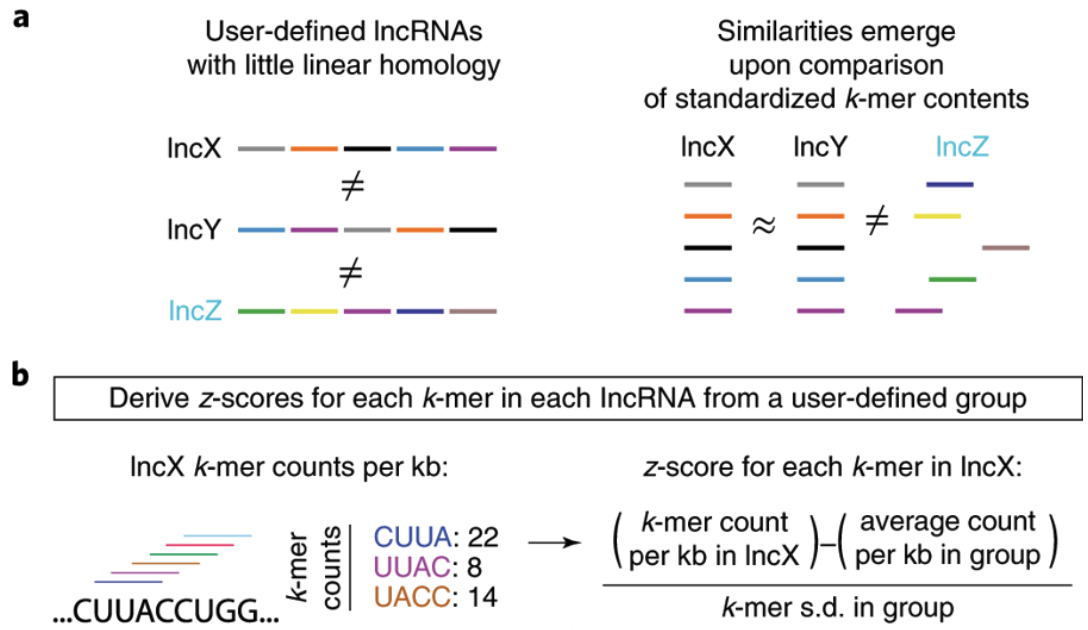
\includegraphics[width=.8\textwidth]{images/seekrclip.png}
\caption[SEEKR Algorithm]{(A) LncRNAs of related function (names in black) may harbor similar sequence similarity in the form of motif content (colored bars) even if they lack linear homology. (B) In SEEKR, the abundance of all kmers of length k are counted by tiling across each lncRNA in a user-defined group in one nucleotide increments. \cite{Kirk2018FunctionalContent}.}
\label{fig:seekr}
\end{figure}

Our lab developed an algorithm for comparing $k$-mer content between lncRNAs, named SEEKR (SEquence Evaluation from $k$-mer Representation). Within the algorithm, each $k$-mer in a sequence is counted through a 1bp sliding window. $k$-mer counts for each lncRNA are then normalized by lncRNA length and standardized across a reference set (\emph{e.g.} the transcriptome) to derive a matrix of standardized $k$-mer frequencies. The degree of similarity between two lncRNA transcripts can then be calculated using the pearson correlation coefficient \cite{Kirk2018FunctionalContent}.


\section{Hidden Markov Models}
A hidden markov model (HMM) is a generative probabilistic model for stochastic sequential processes \cite{Rabiner1989ARecognition,Burge1997PredictionDNA}. For some observable process, or sequence, $X = \{x_1,x_2,\dots, x_n\}$, we assume there is an underlying, or latent, random process $Y = \{y_1,y_2,\dots,y_n\}$ that is controlling the behavior of $X$. A generative probabilistic model such as an HMM calculates the joint probability distribution $P(X,Y)$, rather than the more commonly seen classifier, or discriminative model, that models the conditional probability distribution $P(Y|X)$. Modeling the joint distribution $P(X,Y)$ allows an HMM to not only calculate the probability of any given sequence, but allows for generation of stochastic realizations of the model, \emph{i.e.} an HMM can generate stochastic sequences that behave similarly to the data the model was trained on. HMMs therefore reflect a simplified, hypothesized process by which the data may be reasonably generated. Comparatively, most discriminative classifiers simply attempt to map a data point $x_i$ to some class label $y_j$, $x_i\mapsto y_j$ \cite{Ng2002OnBayes}.

To allow for tractable calculation of probabilities, an HMM relies on the Markov assumption, which states that the current observation is conditionally independent of all other observations, except for the observation immediately prior. This assumption is formally defined in Equation \ref{eq:markov} \cite{Rabiner1989ARecognition}.

\begin{equation}
    P(x_t|x_{t-1},x_{t-2},\dots,x_1) = P(x_t | x_{t-1})
\label{eq:markov}
\end{equation}

This assumption appears simplistic, but it is often sufficient for many modeling tasks that would be impossible without simplifying assumptions. HMMs have been used in many fields, from weather prediction to text prediction, such as a common search engine query \emph{e.g.}: 

\begin{center}
    $P(\texttt{park} | \texttt{dog,nearest,the,where's}) > P(\texttt{office} | \texttt{dog,nearest,the,where's}) $
\end{center}

Could be accurately modeled with the markov assumption:

\begin{center}
    $P(\texttt{park} | \texttt{dog}) > P(\texttt{office} | \texttt{dog}) $
\end{center}

A markov based model would be able to reliably suggest the word \emph{park} instead of \emph{office} because the word \emph{office} would almost never follow the word \emph{dog}, regardless of the remainder of the sentence. This assumption has proven to be wildly useful in the field of bioinformatics, especially with probabilistic modeling of DNA sequences. Mammalian chromosomes can be hundrends of millions of basepairs long, but in reality the relationships between nucleotides exist on much shorter scales. Often a nucleotide can be accurately predicted from preceeding sequence using only the previous 5-6 nucleotides \cite{Burge1997PredictionDNA}.

\subsection{Gene finding and other applications}
HMMs have been used for many purposes, from sequence alignment \cite{Wheeler2013Nhmmer:HMMs} to modeling the timing of switches in fluorescence from FRET experiments \cite{Sgouralis2017AnAnalysis}. An early application of HMMs to biological data was gene finding in the 1990s \cite{Burge1997PredictionDNA}. During this period the Human Genome Project was well underway, and only a fraction of protein coding genes were known. Huge regions of the human genome were being sequenced but massively parallel RNA sequencing technology did not exist at the time, so it was unknown how many novel genes were in the human genome. Therefore, computational models were developed to predict regions within the genome that contained reading frames. 

The majority of the methods developed utilized HMMs at their core \cite{Burge1997PredictionDNA,Pachter2002ApplicationsProblems,Henderson1997FindingModel}. The reason for this was relatively straightforward. Protein coding genes are composed of distinct functional domains, and each of these functional domains contains unique nucleotide distributions \cite{Burge1997PredictionDNA,Pachter2002ApplicationsProblems,Henderson1997FindingModel}. Therefore, we can start with a very general model of protein coding gene:

\begin{center}
    Promoter$\rightarrow$5' UTR$\rightarrow$Exon$\rightarrow$Intron$\rightarrow \dots \rightarrow$ 3' UTR
\end{center}

Using the nomenclature defined in 1.4.1, this is the sequence of hidden states $Y$. The actual DNA sequence that we observe, $X$, is controlled by the presence of these functional domains, and an HMM calculates the joint probability of the parse of the sequence $Y$ and the sequence $X$, or $P(X,Y)$. A parse is here is defined as taking a string of symbols, \textit{e.g.} nucleotides in a sequence, and identifying which portions of that string correspond to a set of predefined functional states. The idea is that some parses of $X$ will be more likely than others, and that the model can be used to identify the most likely parse, $Y^*$, of the data. 
\begin{figure}[h]
\centering
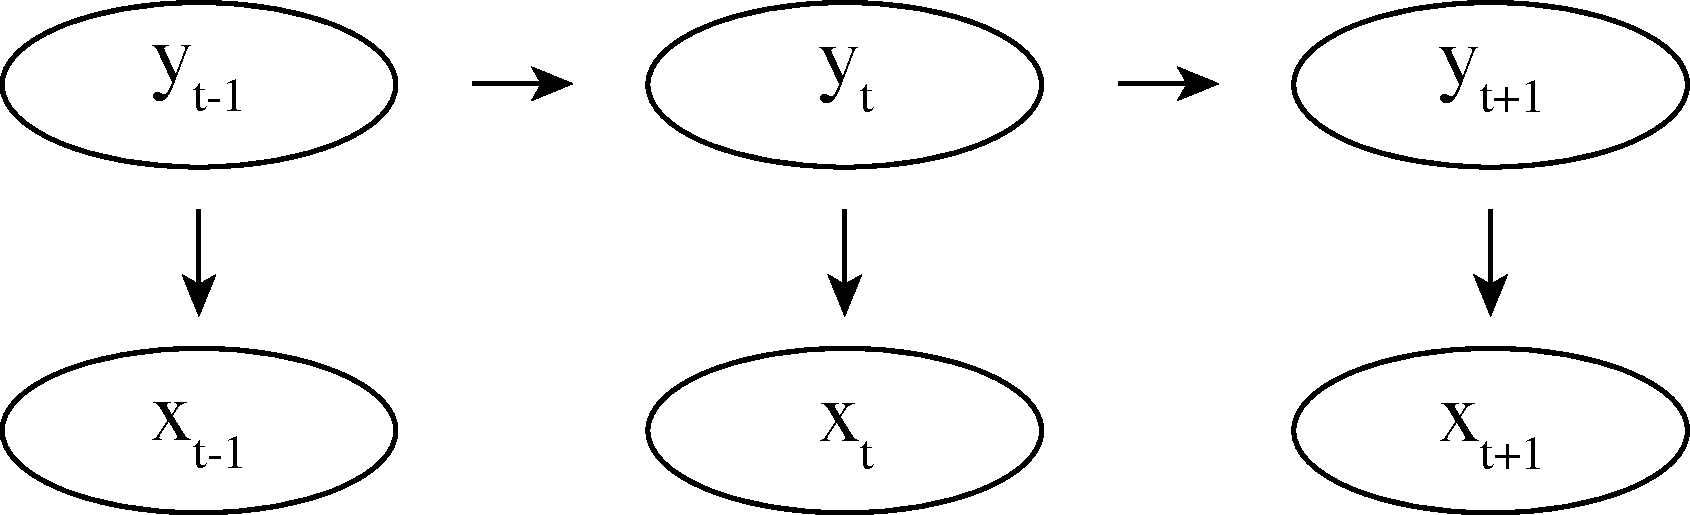
\includegraphics[width=.75\textwidth]{images/hmm.pdf}
\caption{Conditional dependencies in a hidden markov model.}
\label{fig:HMM}
\end{figure}
\subsection{Model structure}
The HMM is constructed with the Markov assumption placed on the sequence of hidden states $Y$, so that for a sequence of length $L$ the probability of the current hidden state $y_t$ is dependent only on the previous hidden state $y_{t-1}$. Further, $y_t$ does not depend on the observed sequence $X$. 
\begin{equation}
    P(y_t,X_{1:L},Y_{1:t-1},Y_{t+1:L}) = P(y_t|y_{t-1})
\end{equation}

And the probability of each observation $x_t \in X$ is conditionally independent of everything except the emitting state at time $t$, $y_t$, and is not dependent on any other observation.

\begin{equation}
    P(x_t,X_{1:t-1},X_{t+1:L},Y_{1:L}) = P(x_t|y_t)
\end{equation}

These conditional independence assumptions can be represented in the graphical form illustrated in Figure \ref{fig:HMM}. 

From here the joint probability for an HMM can be derived \cite{Rabiner1989ARecognition}. This explicitly allows the calculation of the probability for all possible sequences of observations and all possible sequences of hidden states. 

\begin{equation}
    P(X,Y) = P(y_1)p(x_1|y_1)\prod_{t=2}^L{P(y_t|y_{t-1})P(x_t|y_t)}
\label{eq:jointhmm}
\end{equation}

This joint probability distribution allows us to work with the three most common tasks that HMMs are used for: evaluation, decoding, and learning.
\subsection{Inference and Algorithms}
There are three primary questions that an HMM is used to answer. 

\begin{enumerate}
    \item Evaluation: What is the probability of being in a given state, at a particular point in time? A related quantity is the total probability of the observed sequence, \emph{i.e.} $P(X)$. This value is crucial from converting the joint distribution to conditional distributions, especially with respect to Baye's Theorem and the calculation of maximum likelihood estimates for parameters.
    \item Decoding: What is the most likely parse of the sequence? 
    \item Learning: What are the most likely set of parameters, given the observed data?
\end{enumerate}

\subsubsection{Combinatorial Explosion}
To answer the above questions through complete enumeration over all possible combinations of observed sequences and the corresponding possible sequences of hidden states, $K^L$ combinations would have to explored \cite{Rabiner1989ARecognition}, where $L$ is the length of the sequence and $K$ is the number of hidden states. For an average gene of $L=1000$bp and 5 hidden states, $5^{1000}\approx10^{698}$, total calculations would have to be made. This is clearly intractable, even for far shorter sequences. Fortunately algorithms have been developed that make these calculations linear with respect to the length of the sequence \cite{Rabiner1989ARecognition}. 

\subsubsection{Observation Likelihood}
A key quantity when working with HMMs is the total likelihood of the observed sequence $P(X)$. Specifically, we want to know the probability of the observed sequence over \emph{all possible parses} $\phi_i \in \Phi$. Here $\Phi$ refers to the set of all possible parses, and $\phi_i$ refers to an individual parse selected from $\Phi$. 

\begin{equation}
 P(X) = \sum_{\phi_i \in \Phi}{P(X,\phi_i)}  
\label{eq:partition}
\end{equation}

To make it more clear what this quantity is, an example is provided. Let $X = ATC$, an arbitrary DNA sequence, and let the set of hidden states be two labels, $\left\{0,1\right\}$. The set of \emph{all possible parses} $\Phi$ is then a set of $2^3$ elements, and represents all possibles ways that each observation in $X$ can be labeled:

$$\Phi = \{\{000\},\{001\},\{010\},\{011\},\{100\},\{101\},\{110\},\{111\}\}$$

A randomly chosen parse $i$ from this set, $\phi_i \in \Phi$ could be

$$\phi_i = \{010\}$$

Using equation \ref{eq:jointhmm}, there is a joint probability of observing $X=ATC$ and $Y = \phi_i = 010$.

$$P(X=ATC,Y=010)$$

Given that X is fixed, there are still 7 other joint probabilities for each of the remaining possible parses

$$P(X=ATC,Y=000)$$
$$\vdots$$
$$P(X=ATC,Y=111)$$

The law of total probability (Eq. \ref{eq:totalprob}) states that, for two random variables $A$ and $B$ with a joint distribution $P(A,B)$ the marginal distribution $P(A)$ can be calculated by summing over all possible values of $B$ \cite{Brookes1951FoundationsProbability}.

\begin{equation}
    P(A) = \sum_B{P(A,B)}
\label{eq:totalprob}
\end{equation}

Within the context of our HMM, we are interested in knowing the probability of our observation $X=ATC$ regardless of the actual parse. To do this, we apply equation \ref{eq:totalprob} and sum each of the joint probabilities above to get the probability that $X=ATC$, yielding equation \ref{eq:partition}.

This quantity is important for several reasons, but as described above is impossible to calculate through a brute force approach, as the size of the set $\Phi$ combinatorally explodes.

Fortunately, there exists an algorithm which can efficiently calculate $P(X)$ with a computational complexity of $LK^2$, compared to the $K^L$ complexity described above \cite{Rabiner1989ARecognition}.
\subsection{Forward and Backward Algorithms}
\subsubsection{Forward Algorithm}
The forward algorithm recursively calculates the total probability of the sequence $X$ starting from the first observation. This calculation is made feasible by using the conditional independence relationships demonstrated in Figure \ref{fig:HMM} and the joint probability distribution in equation \ref{eq:jointhmm}.

\subsubsection{Initialization}
\begin{equation}
    \alpha_i(t) = p(x_1|y_i)p(y_i)
\label{eq:fwdinit}
\end{equation}

\subsubsection{Induction}
$2\leq t\leq L$
\begin{equation}
    \alpha_i(t) =p(x_t|y_i)\sum_{j}{p(y_i|y_j)\alpha_j(t-1)}
\label{eq:fwdinduc}
\end{equation}

\subsubsection{Termination}
\begin{equation}
    P(X)= \sum_i{\alpha_i(t=L)}
\label{eq:fwdterm}
\end{equation}

Here $i$ and $j$ represent any single hidden state (in a programming environment, it represents the current hidden state under consideration in a \texttt{for} loop through the list of all hidden states). $\alpha_i(t)$ reads as the probability of the sequence $X$ ending at state $i$ at time $t$. The final term, summed over all hidden states, represents the total probability of the observed sequence $X$ \cite{Rabiner1989ARecognition}.

\subsubsection{Backward Algorithm}
The backwards probability $\beta$ is the probability of seeing the observations from time t + 1 to the end, given
that we are in state i at time t ($\beta_i(t)$) \cite{Rabiner1989ARecognition}.

\subsubsection{Initialization}
\begin{equation}
    \beta_i(t=L) = 1
\label{eq:bwdinit}
\end{equation}

\subsubsection{Induction}
$T-1\leq t\leq 1$
\begin{equation}
\beta_i(t-1) =p(x_{t-1}|y_i)\sum_{j}{p(y_i|y_j)\beta_j(t)}
\label{eq:bwdinduc}
\end{equation}

\subsubsection{Termination}
\begin{equation}
    P(X)= \sum_i{\beta_i(t=1)} = \sum_i{\alpha_i(t=L)}
\label{eq:bwdterm}
\end{equation}

The forward and backward algorithms can be combined to calculate the probability of being in any hidden state $i$ at any position within the sequence, \emph{i.e.} $P(Y_t=i|x_{1:L})$. The reason both equations are used is that it allows for information prior to the observation as well as information posterior to observation to be considered. 

\begin{equation}
p(y_t=i|x_{1:L}) = \frac{\alpha_i(t)\beta_i(t)}{\sum_j{\alpha_j(t)\beta_j(t)}}
\label{eq:fwdbwd}
\end{equation}

\begin{figure}[t]
\centering
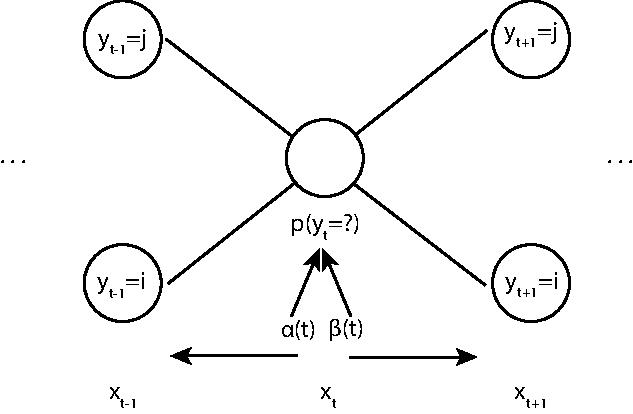
\includegraphics[width=.75\textwidth]{images/fwdbwd.pdf}
\caption[Forward-backward smoothed probability]{Information from the entire sequence $x_{1:T}$ is incorporated through the forward and backward probabilities. The formal definition of this probability is defined in equation \ref{eq:fwdbwd}}
\label{fig:fwdbwd}
\end{figure}

Figure \ref{fig:fwdbwd} illustrates how information from the entire sequence is incorporated through the forward probability, $\alpha$, and the backward probability, $\beta$, to get a \emph{smoothed probability} for $y_t = i$.

\subsection{Viterbi Algorithm}
Perhaps one of the most useful tasks for an HMM is that of decoding, or identifying the most likely parse of the sequence, $\phi_{max}$. That is, $\phi_{max}$ yields the highest joint probability $P(X,Y=\phi_{max})$ \cite{Rabiner1989ARecognition}. 

Mathematically, the Viterbi algorithm is very similar to the forward algorithm. Rather than taking the sum at each step in the recursion, instead the state transition that maximizes the probability at time $t$ is stored in a list, and then a back-trace is calculated yielding the path of maximizing hidden states.

\subsubsection{Initialization}
Calculate the probability for each state at time $t=1$, $\mu_i(t=1)$, and initialize a list with each state, $V_i(t=1)$
\begin{equation}
    \mu_i(t=1) = \max_i p(x_1|y_i)p(y_i)
\label{eq:fwdinit}
\end{equation}
$$    V_i(t=1) = i$$
\subsubsection{Induction}
Calculate the probability of being in each state $i$ at time $t$, after transitioning from state $j$ at time $t-1$, then save the largest probability $\mu_i(t)$ for each state. $\mu_i(t)$ reads as the largest probability for the sequence $X$ to end in state $i$ at time $t$ following a transition from state $j$ at time $t-1$ \cite{Rabiner1989ARecognition}. 
\begin{equation}
    \mu_i(t) =\max_j\left[p(x_t|y_i)p(y_i|y_j)V_j(t-1)\right]
\label{eq:fwdinduc}
\end{equation}

Then, for each state $i$, save the state transition $j\rightarrow i$ that maximized $\mu_i(t)$.  
$$V_i(t) =\argmax_j\left[p(x_t|y_i)p(y_i|y_j)V_j(t-1)\right]$$

\subsubsection{Termination}
The probability of the most likely end state is then
\begin{equation}
    P^*(t=L) = \max_i{\mu_i(t=L)}
\label{eq:fwdterm}
\end{equation}
And the back-trace for the Viterbi most likely path is initialized at the last observation $t=L$:
$$V^*(t=L) = \argmax_i{P^*(t=L)}$$
At time $t=L-1$, we then retrieve $V^*(t=L-1)$, which is the state that transitioned to the known maximizing state at the end of the sequence $V^*(t=L)$. This recursion is then repeated to the beginning of the sequence.
\begin{equation}
V^*(t-1) = \argmax_i{\mu_i(t)}
\label{eq:backtrace}    
\end{equation}

Once the list created from equation \ref{eq:backtrace} has been inverted, as it is a back-trace, the path $V^* = \phi_{max}$, which is the parse $\phi \in \Phi$ that maximizes the joint probability of the HMM \cite{Rabiner1989ARecognition}.

\subsection{Baum-Welch Algorithm}
A final common task for HMMs is to learn the set of parameters that maximize the likelihood of the model, \textit{i.e.} what set of parameters $\theta = \{A=$transition parameters,$E=$emission parameters,$\pi=$initiation parameters$\}$, maximize the probability of the observed sequence $P(X|\theta)$. The Baum-Welch algorithm does this through an expectation-maximization (EM) algorithm that estimates a new set of parameters, $\theta^*$, by iterating through the forward and backward algorithms, and then calculation of the new likelihood $P(X|\theta^*)$ using the updated parameter values. This algorithm is guaranteed to converge to a \textit{local} maximum -- not necessarily a global maximum, meaning that better estimates for the parameters may exist. Furthermore, it is possible for the Baum-Welch algorithm to overfit the data, \textit{i.e.} $P(X|\theta^{\texttt{MLE}}) > P(X|\theta^{\texttt{true}})$. 

\subsubsection{Initiation}
Any value, including randomized values, can be initially assigned to the parameter values in $\theta = \{A,E,\pi\}$, however if \textit{a priori} knowledge exists then that may speed convergence to the MLE. The Baum-Welch algorithm utilizes the forward and backward algorithm, and being described above, will be compressed here.

\subsubsection{Forward and Backward Probabilities }
\begin{enumerate}
\item Calculate the forward probabilities, $\alpha_i(t)$, for each state for each observation, representing the probability of seeing the observations $x_{1:t}$ and ending in state $i$ at time $t$. 
\item Calculate the backward probabilities, $\beta_i(t)$, for each state for each observation, representing the probability of the observations $x_{t+1:T}$ given starting state $i$ at time $t$. 
\item $\sum_i{\alpha_i(T)} = \sum_i{\beta_i(1)} = P(X|\theta)$       
\end{enumerate}

\subsubsection{Update}

1. Calculate the probability of being state $i$ at time $t$, through Bayes theorem: 

$$\gamma_i(t) = \frac{P(y_t = i,X|\theta)}{P(X|\theta)}= \frac{\alpha_i(t)\beta_i(t)}{\sum_j{\alpha_j(t)\beta_j(t)}}$$
2. Calculate the probability of transitioning from state $i$ at time $t$ to state $j$ at time $t+1$ 

$$\epsilon_{ij}(t) = P(y_t =i,y_{t+1}=j|X,\theta) = \frac{P(y_t = i,y_{t+1}=j,X|\theta)}{P(X|\theta)} = \frac{\alpha_i(t)A_{ij}\beta_j(t+1)E_j(x_{t+1})}{\sum_j{\alpha_j(t)\beta_j(t)}}$$ 
3. Calculate the expected number of transitions from state $i$ to state $j$ relative to the expected occurrence of $i$ over the length of $X$, and update the transition matrix $A$ accordingly. 

$$A_{ij}^* = \frac{\sum_{t=1}^{T-1}{\epsilon_{ij}(t)}}{\sum_{t=1}^{T}{\gamma_i(t)}}$$ 4. Calculate the expected number of occurrences of each observation category in the emission distribution (in the use-case in this dissertation, all $k$-mers), ``v'' (an observation in $X$) in state $i$, relative to the total occurrence of state $i$. 

$$E_i^*(v) = \frac{\sum_{t=1}^T{1_{x_t=v}}\gamma_i(t)}{\sum_{t=1}^T{\gamma_i(t)}}$$ Where $1_{x_t=v}$ is an indicator that equals 1 if $x_t = v$, and 0 otherwise. 



\subsubsection{}


\begin{singlespace}
\printbibliography[heading=bibintoc,title={References}]
\end{singlespace}
\chapter{Xist and Rsx}
The sex chromosomes of therian (eutherian and metatherian) mammals evolved from a pair of identical autosomes after the split of therian and monotreme mammals from their most recent common ancestor. Since that divergence, the Y chromosome has lost the large majority of its protein coding genes, creating a gene dosage imbalance between XY males and XX females. Part of the system that compensates this imbalance is a process known as X-chromosome Inactivation (XCI). Initiated early during female development, XCI results in the transcriptional silencing of one X chromosome in each somatic cell in female mammals. In eutherians, XCI is mediated by a long non-coding RNA (lncRNA) called \textit{\emph{Xist}} \cite{Balaton2018TheChromosome,Brockdorff2018LocalNcRNA,DaRocha2017NovelConformation,Sahakyan2018TheCompensation}. 

The silencing function of \textit{\emph{Xist}} is thought to be mediated by the concerted action of several domains of tandemly repeated sequence that are interspersed throughout its length. These repeat domains harbor binding sites for distinct subsets of proteins that, through incompletely understood mechanisms, help \textit{\emph{Xist}} achieve different aspects of its function. “Repeat A” binds proteins called SPEN and RBM15, and is required for the stabilization of spliced \textit{\emph{Xist}} RNA, and for \emph{Xist} to silence actively transcribed regions of the X chromosome \cite{Chu2015SystematicProteins,Engreitz2013TheChromosome, Hoki2009AMouse,McHugh2015TheHDAC3, Moindrot2015ASilencing, Patil2016M6Repression,Royce-Tolland2010TheInactivation,Wutz2002ChromosomalRNA}. “Repeat B”, and at least a portion of “Repeat C”, bind HNRNPK to recruit the Polycomb Repressive Complex 1 (PRC1) to the inactive X chromosome \cite{Almeida2017PCGF3/5-PRC1Inactivation,Pintacuda2017HnRNPKSilencing}. “Repeat E” binds many proteins, including CIZ1, and is required for the stable association of \emph{Xist} with X-linked chromatin and for the sustained recruitment of Polycomb Repressive Complex 2 (PRC2) to the inactive X  \cite{Ridings-Figueroa2017TheTerritory,Smola2016SHAPECells,Sunwoo2017RepeatCIZ1}.

Intriguingly, metatherians (marsupials) may have convergently evolved their own lncRNA, \emph{Rsx}, to mediate XCI in XX females \cite{Grant2012RsxInactivation}. \emph{Rsx} shares no linear sequence similarity with \textit{\emph{Xist}} and is located in a different syntenic block on the marsupial X. Nevertheless, \emph{Rsx} shares a number of surprising similarities with \emph{Xist}. Both \emph{Xist} and \emph{Rsx} are expressed exclusively from the inactive X in females and are retained in the nucleus, forming what has been described as a “cloud-like” structure around their chromosome of synthesis. Moreover, both lncRNAs are spliced yet unusually long in their final processed form, and their expression correlates with the accumulation of histone modifications deposited by the Polycomb Repressive Complexes (PRCs) on the inactive X \cite{Grant2012RsxInactivation}. 

Studies performed over the last three decades indicate that \textit{\emph{Xist}} is required for normal XCI in eutherians \cite{Balaton2018TheChromosome,Brockdorff2018LocalNcRNA,DaRocha2017NovelConformation,Sahakyan2018TheCompensation}. Given the similarities between \emph{Rsx} and \emph{Xist}, it has been proposed that the marsupial \emph{Rsx} is the functional analogue of \emph{Xist} \cite{Grant2012RsxInactivation}. While this hypothesis has yet to be directly tested, expression of an \emph{Rsx} transgene on a mouse autosome does, to a certain extent, induce local gene silencing, supporting the notion that \emph{Rsx} harbors \emph{Xist}-like function \cite{Grant2012RsxInactivation}.

Despite their lack of linear sequence similarity, \emph{Xist} and \emph{Rsx} both harbor long, internal domains of tandemly repeated sequence \cite{Grant2012RsxInactivation,Johnson2018AdaptationGenome}. We recently discovered that evolutionarily unrelated lncRNAs that encode similar functions often harbor non-linear sequence similarity in the form of $k$-mer content, where a $k$-mer is defined as all possible combinations of a nucleotide substring of a given length k \cite{Kirk2018FunctionalContent}. Below, we describe our use of $k$-mer based methods to investigate the possibility that the repeat domains in \emph{Xist} and \emph{Rsx} harbor non-linear sequence similarity that might be suggestive of shared function.

\section{Results}
\subsection{\emph{Xist} and \emph{Rsx} share no local alignments}
\emph{Xist} and \emph{Rsx} are both notable for their domains of highly repetitive sequence, which can be identified by aligning each lncRNA to itself and visualizing the alignment data as a dot plot (\cite{Rice2000EMBOSS:Suite}). In mouse \emph{Xist}, the four major repetitive regions are referred to as Repeats A, B, C, and E (Figure 1A; \cite{Brockdorff10TheNucleus.}). Repeats A, B, and E are conserved in eutherian mammals, whereas Repeat C appears to be specific to murid rodents (Figure 1C;\cite{Nesterova2001CharacterizationSequence,Yen2007AEutheria}). In human \emph{Xist}, the four major repetitive regions are referred to as Repeats A, B, D, and E (Figure 1B; \cite{Brown10TheNucleus.}). Relative to mouse, human Repeat B is comprised of two shorter Repeat B-like regions that appear to have been disrupted by insertion (Figure 1B; \cite{Nesterova2001CharacterizationSequence,Yen2007AEutheria}). Human Repeat D is comprised of eight core repeats flanked by several additional repeats that exhibit partial similarity to its core (Figure 1B; \cite{Brown10TheNucleus.,Nesterova2001CharacterizationSequence,Yen2007AEutheria}). While Repeat D is absent in murid rodents (Figure 1C), Repeat D-like sequence appears in many other mammals (\cite{Nesterova2001CharacterizationSequence,Yen2007AEutheria}).

\begin{figure}[!h]
\centering
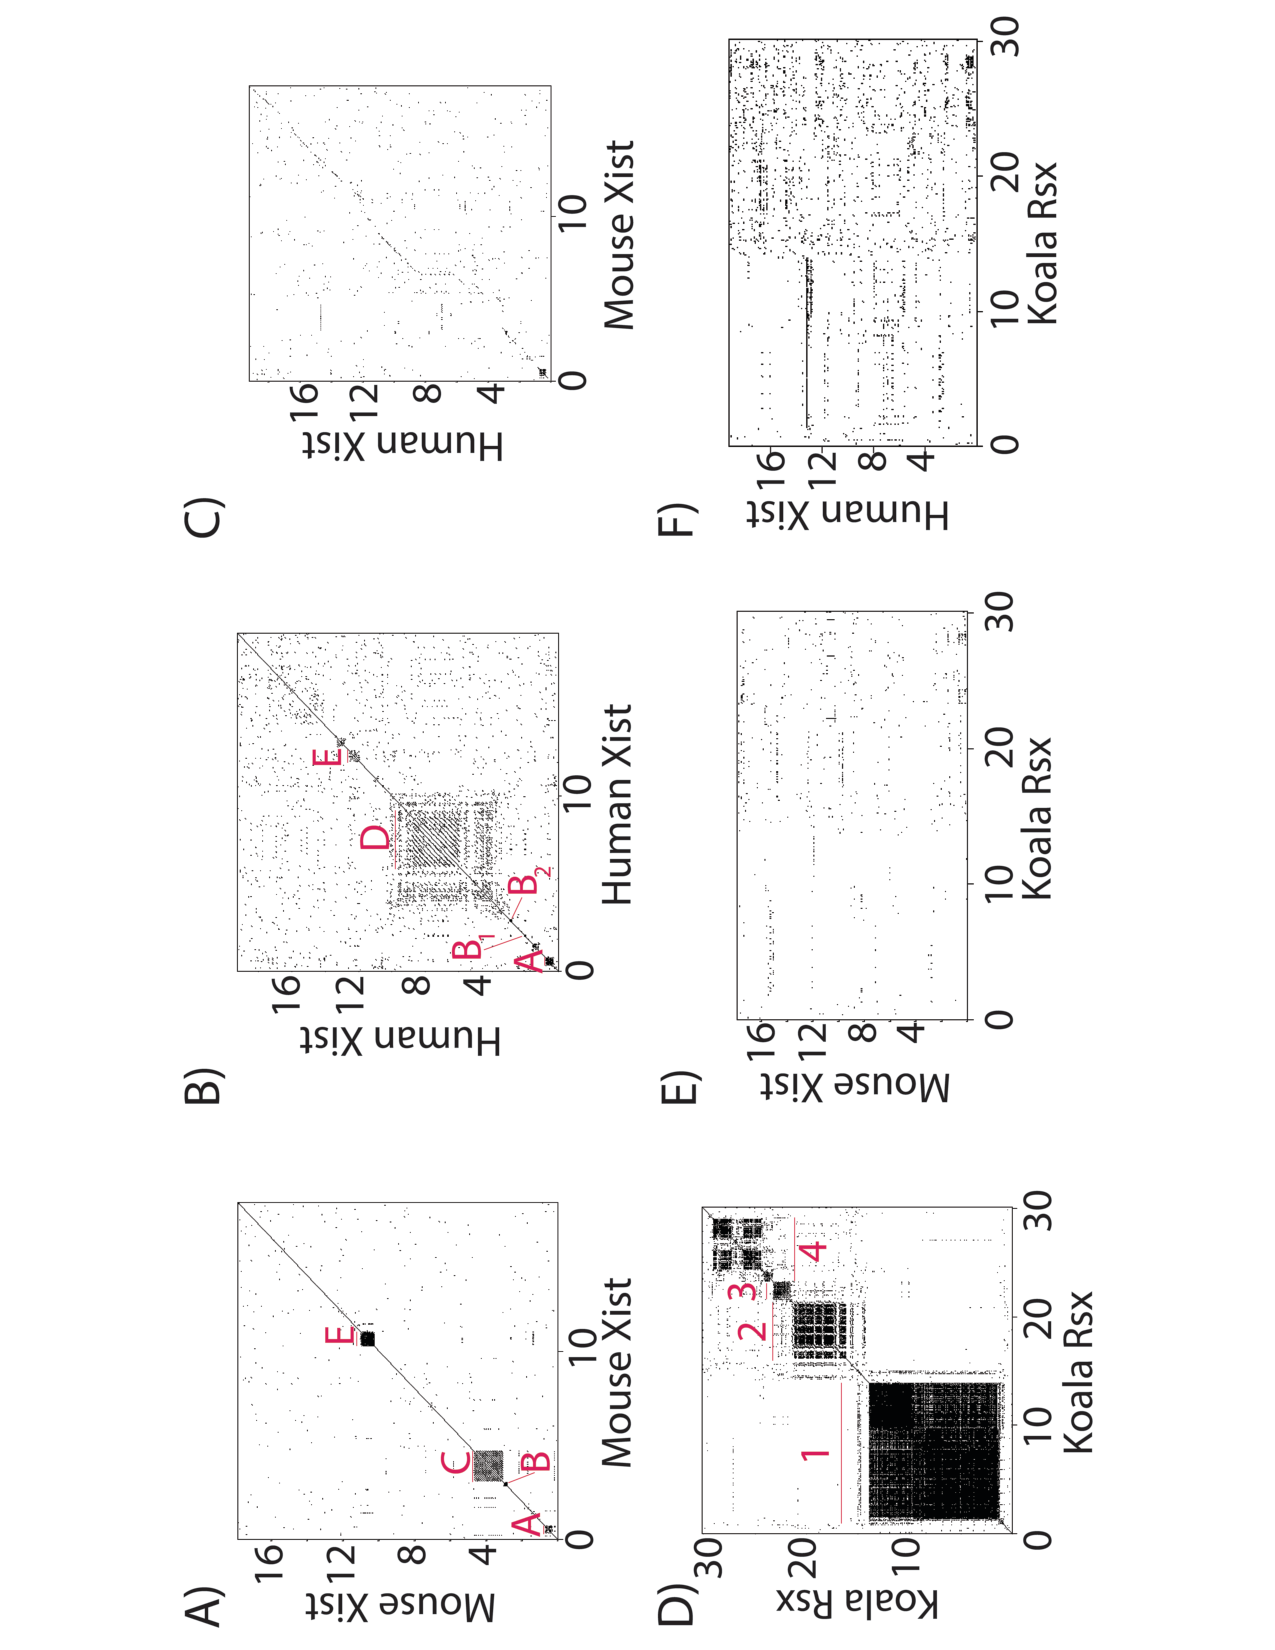
\includegraphics[angle=-90, width=\textwidth]{images/fig1-v2-01.pdf}
\caption[\emph{\emph{Xist}} and \emph{\emph{Rsx}} dot plots]{Dot plots comparing mouse and human \emph{Xist} and \emph{Rsx} to themselves and to each other. The location of repeat domains in all three lncRNA-to-self plots are marked with red bars and names/numbers.}
%\label{fig:x cubed graph}
\end{figure}

In contrast to \emph{Xist}, which is mostly comprised of non-repetitive sequence, nearly all of the sequence in \emph{Rsx} can be assigned to one of four repetitive domains (Figure 1D; \cite{Johnson2018AdaptationGenome}). Here, we refer to the repetitive domains in \emph{Rsx} as Repeats 1 through 4. It has been suggested that \emph{Rsx} Repeat 1 is functionally analogous to \emph{Xist} Repeat A, because both repeats are the first to occur in each lncRNA, and because both repeats contain GC-rich elements \cite{Grant2012RsxInactivation,Johnson2018AdaptationGenome}. Beyond this observation, little is known about the repetitive regions in \emph{Rsx} and how they might relate to those in \emph{Xist}. Hypothesizing that the repeat domains in \emph{Xist} and \emph{Rsx} recruit similar subsets of proteins, we expected that dot plots comparing the sequence of \emph{Xist} to the sequence of \emph{Rsx} would reveal regions of sequence similarity. However, this was not the case (Figure 1E, F), nor was significant similarity between \emph{Xist} and \emph{Rsx} detected using BLASTN or the hidden-markov based nhmmer \cite{Altschul1990BasicTool,Wheeler2013Nhmmer:HMMs}. 

\subsection{Tandem repeats domains in \emph{Xist} and \emph{Rsx} share $k$-mer content}
We hypothesized that sequence similarity between \emph{Xist} and \emph{Rsx} might become apparent using an algorithm we recently developed to detect sequence similarity between evolutionarily unrelated lncRNAs \cite{Kirk2018FunctionalContent}. In our algorithm, called SEEKR (Sequence evaluation through $k$-mer representation), groups of lncRNAs are compared to each other by counting the number of occurrences of each $k$-mer of a given length k in each lncRNA, then normalizing $k$-mer counts by the length of the lncRNA in question, and finally calculating a $z$-score for each $k$-mer in each lncRNA. The list of $z$-scores for each $k$-mer in a lncRNA is referred to as its “$k$-mer profile” and represents the abundance of each $k$-mer in the lncRNA relative to the abundance of each $k$-mer in the other lncRNAs that were analyzed as part of the group. In SEEKR, $k$-mer profiles from lncRNAs of interest are compared to each other using Pearson’s correlation. We previously demonstrated that SEEKR can be used to quantify the similarity between any number of lncRNAs regardless of their evolutionary relationships or differences in their lengths, and that similarities in $k$-mer profiles correlated with lncRNA protein binding potential, subcellular localization, and \emph{Xist}-like repressive activity. A major strength of SEEKR is that it ignores positional information in similarity calculations, allowing it to quantify non-linear sequence relationships \cite{Kirk2018FunctionalContent}. 

In order to compare \emph{Xist} and \emph{Rsx} via SEEKR, we calculated the $k$-mer profile at $k$ = 4 of individual repeat domains in mouse \emph{Xist} and koala \emph{Rsx}, using all mouse lncRNAs from GENCODE as a background set to derive the mean and standard deviation of the counts for each $k$-mer \cite{Derrien2012TheExpression}. The mechanisms through which \emph{Xist} functions have been most extensively studied in mouse \cite{Sahakyan2018TheCompensation}. For this reason, we primarily used the repetitive regions from mouse \emph{Xist} as search features in this work. However, because of the conservation of Repeat D-like domains in non-murid eutherian mammals (\cite{Nesterova2001CharacterizationSequence,Yen2007AEutheria}), we also included the sequence of human \emph{Xist} Repeat D in our analyses. We used the sequence from koala \emph{Rsx} as our exemplar, owing to the high-quality of the koala genome build relative to builds from other marsupials \cite{Johnson2018AdaptationGenome}.

In our previous work, we found that SEEKR performed best when the length of the lncRNA or lncRNA fragment being studied was similar to $4^k$, i.e. the total number of possible $k$-mers at $k$-mer length k. In tests of \emph{Xist}-like repressive activity, we found that comparisons of lncRNAs using $k$-mer lengths of $7$+ underperformed relative to comparisons using smaller $k$-mer lengths, owing to the fact that most annotated lncRNAs are much less than $4^7$ (16384) nucleotides long, and $k$-mer profiles of individual lncRNAs at $k=7$ ($\approx$16384 possible $k$-mers) are dominated by “0” values \cite{Kirk2018FunctionalContent}. Based on this observation, and because Repeats A and B, two essential repetitive regions within \emph{Xist}  \cite{Almeida2017PCGF3/5-PRC1Inactivation,Hoki2009AMouse,Pintacuda2017HnRNPKSilencing,Royce-Tolland2010TheInactivation,Wutz2002ChromosomalRNA}, are each about $4^4$ (256) nucleotides in length, we reasoned that $k$-mer profiles at $k$ = 4 ($4^4$=256 possible $k$-mers) would provide a reasonable estimate of sequence complexity for the repeats without being dominated by “0” values. 

We also noted that relative to most lncRNAs, $k$-mer content in the repetitive regions of \emph{Xist} and \emph{Rsx} was skewed (Figure S2A). We therefore elected to $\log_2$-transform $z$-scores in $k$-mer profiles prior to comparison via Pearson’s correlation, recognizing that this transformation would reduce skew and allow us to evaluate similarity in the context of a log-linear scale (Figure S2B).

The individual repeat domains in \emph{Xist} and \emph{Rsx} vary substantially in terms of their length and sequence complexity. \emph{Xist} repeats tend to be shorter and lower in overall complexity than repeats in \emph{Rsx} (Figure 2A, B). Despite these differences, using SEEKR, we identified substantial levels of similarity between the repeat domains of \emph{Xist} and \emph{Rsx}. The Repeat A region of \emph{Xist} was most similar to \emph{Rsx} Repeat 4, exhibited a weak positive correlation with Repeat 2, and had negative correlations with \emph{Rsx} Repeats 1 and 3 (Pearson’s r of 0.21, for Repeat A versus Repeat 4, respectively, and r of -0.02, 0.09, and -0.08 for Repeats 1, 2, and 3, respectively; Figure 2C). In contrast, \emph{Xist} Repeat B was most similar to \emph{Rsx} Repeat 1 and had negative correlations with \emph{Rsx} Repeats 2 through 4 (Pearson’s r of 0.33 for Repeat B versus Repeat 1; Figure 2C). Repeat C, which is specific to murid rodents (i.e. it is not found in other eutherians), had no appreciable correlation with any \emph{Rsx} repeat, whereas human Repeat D had positive correlations with \emph{Rsx} Repeat 1 and 4 (r of 0.20, 0.12, respectively; Figure 2C). The $k$-mer profile of \emph{Xist} Repeat E had positive correlations that increased progressively in \emph{Rsx} Repeats 2, 3, and 4. (Pearson’s r of 0.15, 0.25, 0.40, respectively; Figure 2C). 

\begin{figure}[!h]
\centering
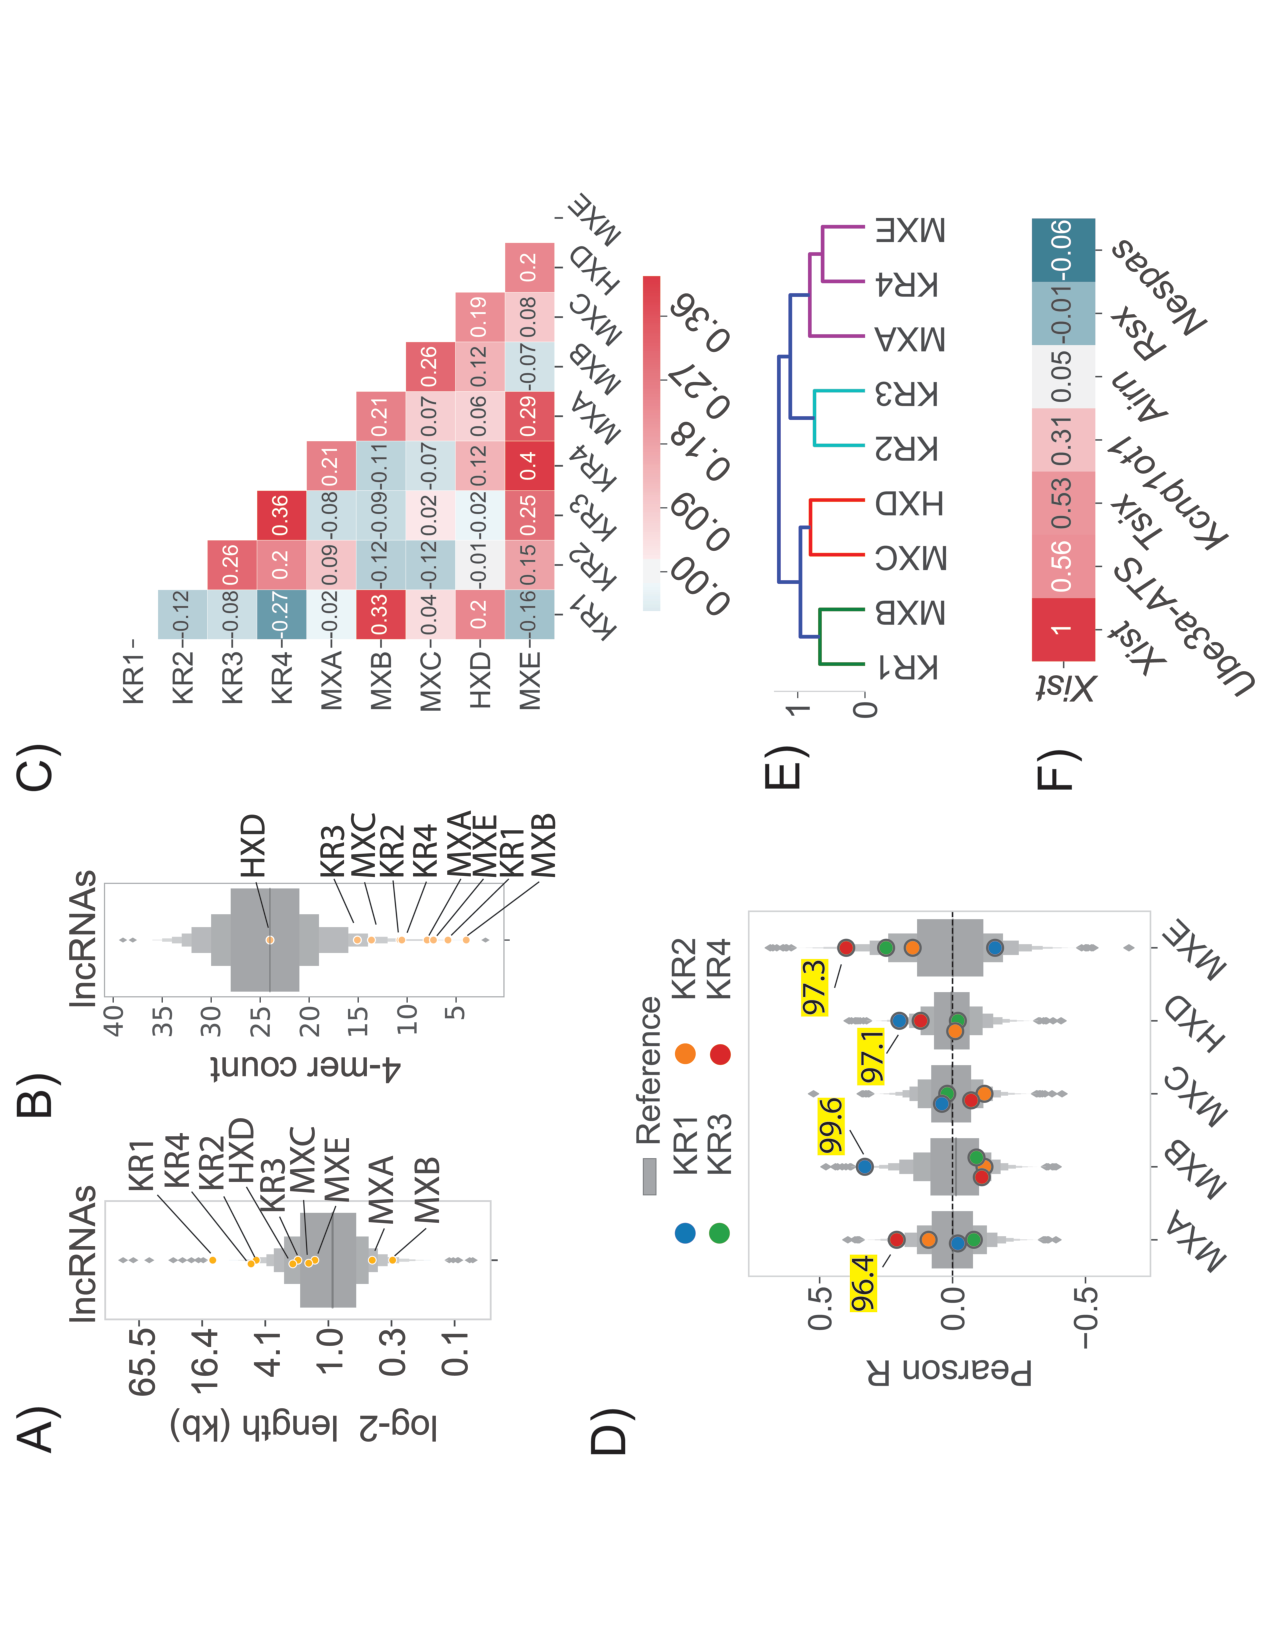
\includegraphics[angle=-90,width=.8\textwidth]{images/fig2_-01.pdf}
\caption[Domain based sequence similarity]{Length of \emph{Xist} and \emph{Rsx} repeat domains and (B) sequence complexity estimated by the number of unique 4-mers that constitute 25\% of the total 4-mer counts in a transcript, each relative to all other GENCODE M18 lncRNA transcripts. For panels A – E: “M”, “H”, and “K” signify mouse, human, and koala, respectively, “X” and “R” signify \emph{Xist} and \emph{Rsx}, respectively, and the final letter or number in each abbreviation signifies the repeat domain in question. (C) Correlation matrix displaying the Pearson’s r value derived from comparing $k$-mer profiles at $k$ = 4 of each of the four repeat domains in koala \emph{Rsx} (Repeats 1 – 4), the major repeats in mouse \emph{Xist} (Repeats A, B, C, E), and human \emph{Xist} Repeat D. The set of mouse lncRNAs from GENCODE was used to derive mean and standard deviation values for length normalized abundance of each $k$-mer. (D) Similarity of repeat domains in \emph{Xist} and \emph{Rsx} relative to all lncRNA transcripts in the mouse GENCODE M18 database \cite{Derrien2012TheExpression}. Each subplot shows the distribution of Pearson’s r values describing the similarity between the \emph{Xist} repeat in question and the set of GENCODE lncRNA transcripts. Similarities between \emph{Xist} and \emph{Rsx} that are above the $95^{th}$ percentile of similarity for all mouse lncRNAs are highlighted in yellow. (E) The correlation matrix in (A) subject to hierarchical clustering. Colors represent clusters for all descendent links beneath the first node in the dendrogram with distance less than 70\% of the largest distance between all clusters. (F) SEEKR- derived similarity (in the form of Pearson’s r; \cite{Kirk2018FunctionalContent}) between full-length \emph{Xist}, other cis- repressive lncRNAs in mouse, and koala \emph{Rsx} \cite{Johnson2018AdaptationGenome}}. 
%\label{fig:x cubed graph}
\end{figure}

We sought to quantify the strength of the similarity between repeat domains in \emph{Xist} and \emph{Rsx} relative to other mouse lncRNAs. To do this, we used Pearson’s correlation to compare the $k$-mer profile of each \emph{Xist} repeat domain to the $k$-mer profiles of the set of spliced GENCODE M18 mouse lncRNAs \cite{Derrien2012TheExpression}. We compared this distribution of Pearson’s r values to the r value obtained when comparing each \emph{Xist} repeat to each \emph{Rsx} repeat. 

This analysis revealed striking similarities between the repeat domains of \emph{Xist} and \emph{Rsx}. \emph{Xist} Repeat B was more similar to \emph{Rsx} Repeat 1 than it was similar to 99.6\% of all lncRNAs (similarity ranked 65th out of 17523 comparisons), despite the fact that the two repeats differ in length by ~50-fold (Figures 2A, D; Tables S1, S2). \emph{Xist} Repeat A was more similar to \emph{Rsx} Repeat 4 than it was similar to 96.4\% of all other lncRNAs (its similarity ranked 626nd out of 17523 comparisons), \emph{Xist} Repeat D was more similar to \emph{Rsx} Repeat 1 than it was similar to 97.1\% of all other lncRNAs (its similarity ranked 515th out of 17523 comparisons), and \emph{Xist} Repeat E was more similar to \emph{Rsx} Repeat 4 than it was similar to 97.3\% of all other lncRNAs (its similarity ranked 467th out of 17523 comparisons; Figure 2D; Table S1, S2). No other repeat domains in \emph{Xist} and \emph{Rsx} fell above the $95^{th}$ percentile in terms of their similarity to each other. Similar trends were observed when we used $k$-mer lengths $k = 4$, 5 and 6 for this analysis (Figure S3A). 

Current models suggest that the tandem repeats in \emph{Xist} have distinct functions \cite{Balaton2018TheChromosome,Brockdorff2018LocalNcRNA,DaRocha2017NovelConformation,Sahakyan2018TheCompensation}. Thus, we were surprised to find that the repeat domains within \emph{Xist} also exhibited high levels of similarity to each other (Table S1, S2). Repeat A was more similar to Repeat E than it was similar to 99.6\% of all lncRNAs. Likewise, Repeats B and C were more similar to each other than they were similar to 97.8\% and 99.6\% of all other lncRNAs, respectively. Finally, Repeats C and D were more similar to each other than they were similar to 97.0\% and 96.2\% of all other lncRNAs, respectively (Table S1, S2). 

The similarities between specific domains of \emph{Xist} and \emph{Rsx} were also evident in an unsupervised hierarchical cluster of the matrix from Figure 2C. \emph{Xist} Repeat B and \emph{Rsx} Repeat 1 formed a basal cluster which joined with a second basal cluster comprising \emph{Xist} Repeat C and \emph{Xist} Repeat D.   \emph{Rsx} Repeat 4 and \emph{Xist} Repeat E formed a basal cluster that that joined with \emph{Xist} Repeat A. This multilevel cluster (\emph{Rsx} Repeat 4, \emph{Xist} Repeat E, and \emph{Xist} Repeat A) joined with another basal cluster comprising \emph{Rsx} Repeats 2 and 3 (Figure 2E). 

At $k$-mer length $k = 4$, Pearson’s correlation with and without log-transformation of $k$-mer $z$-scores, as well as Spearman’s correlation of non-transformed $z$-scores, detected similar relationships between \emph{Xist} and \emph{Rsx} repeat domains (Figure S4). While the similarities between individual domains were still evident at higher $k$-mer lengths, particularly when using Pearson’s correlation of log-transformed $k$-mer counts, the clustering patterns that we observed at $k$-mer length $k = 4$ began to dissolve (Figure S4). At high $k$-mer lengths, Spearman’s correlation was the least informative method of comparison, owing to the large number of ``zero” values that populate $k$-mer profiles at these lengths (Figure S4). Thus, to a certain extent, the similarities in the repeat domains of \emph{Xist} and \emph{Rsx} are detectable regardless of prior assumptions about log-linear, linear, and monotonic relationships between $k$-mer profiles. However, the most robust similarities are detected using Pearson’s correlation of log-transformed $k$-mer counts (Figure S4).
We observed that the similarities between \emph{Xist} and \emph{Rsx} were obscured when the $k$-mer profiles of the full-length lncRNAs were compared to each other (Pearson’s r of -0.01 for the comparison of full-length \emph{Xist} to full-length \emph{Rsx}; Figure 2F). This loss of similarity highlights the utility of domain-based similarity searches, particularly for lncRNAs whose functional domains may comprise a fraction of their overall length. The dissimilarity between $k$-mer profiles of full-length \emph{Xist} and full-length \emph{Rsx} likely stems from the fact that virtually all of \emph{Rsx} is comprised of repetitive sequence domains that harbor limited $k$-mer diversity relative to the non-repetitive sequence of \emph{Xist} (Figure 2B and compare Figures 1A-C to 1D). 

\subsection{Tandem repeat sequence properties}
Qualitative similarities between \emph{Xist} and \emph{Rsx} repeat domains were also revealed using MEME to visualize motifs that were enriched within individual domains \cite{Bailey2009MEMESearching}. In \emph{Xist} Repeat A, MEME identified one motif comprised of short runs of G and C nucleotides and one motif most notable for runs of T nucleotides (Figure 3A). Similar patterns were seen in the motifs enriched in \emph{Rsx} Repeat 4 (Figure 3B). The single motif from Repeat B was almost exclusively comprised of two tandemly arranged ‘GCCCC’ motifs, and motifs containing runs of ‘G’ and ‘C’ nucleotides could be seen in \emph{Rsx} Repeat 1 (Figure 3A, B). The pyrimidine-rich runs that were characteristic of \emph{Xist} Repeat E were also observed \emph{Rsx} Repeat 4 (Figure 3A, B). \emph{Rsx} Repeat 2 was unique in its enrichment of AAAG and GAAA motifs (Figure 3B).
Several of the repeat domains in \emph{Xist} and \emph{Rsx} could be distinguished by the presence of $k$-mers comprised of runs of individual nucleotides that extended for two or more consecutive positions (such as AA, CC, GG, or TT; File S1). Similar to enriched motifs, $k$-mers containing mononucleotide runs may function to recruit different subsets of RNA binding proteins \cite{Dominguez2018SequenceProteins,Ray2013ARegulation}. We therefore sought to quantify the enrichment of $k$-mers containing mononucleotide runs in the repeat domains of \emph{Xist} and \emph{Rsx}, reasoning that this analysis might provide insight into function. 
\begin{figure}[p]
\centering
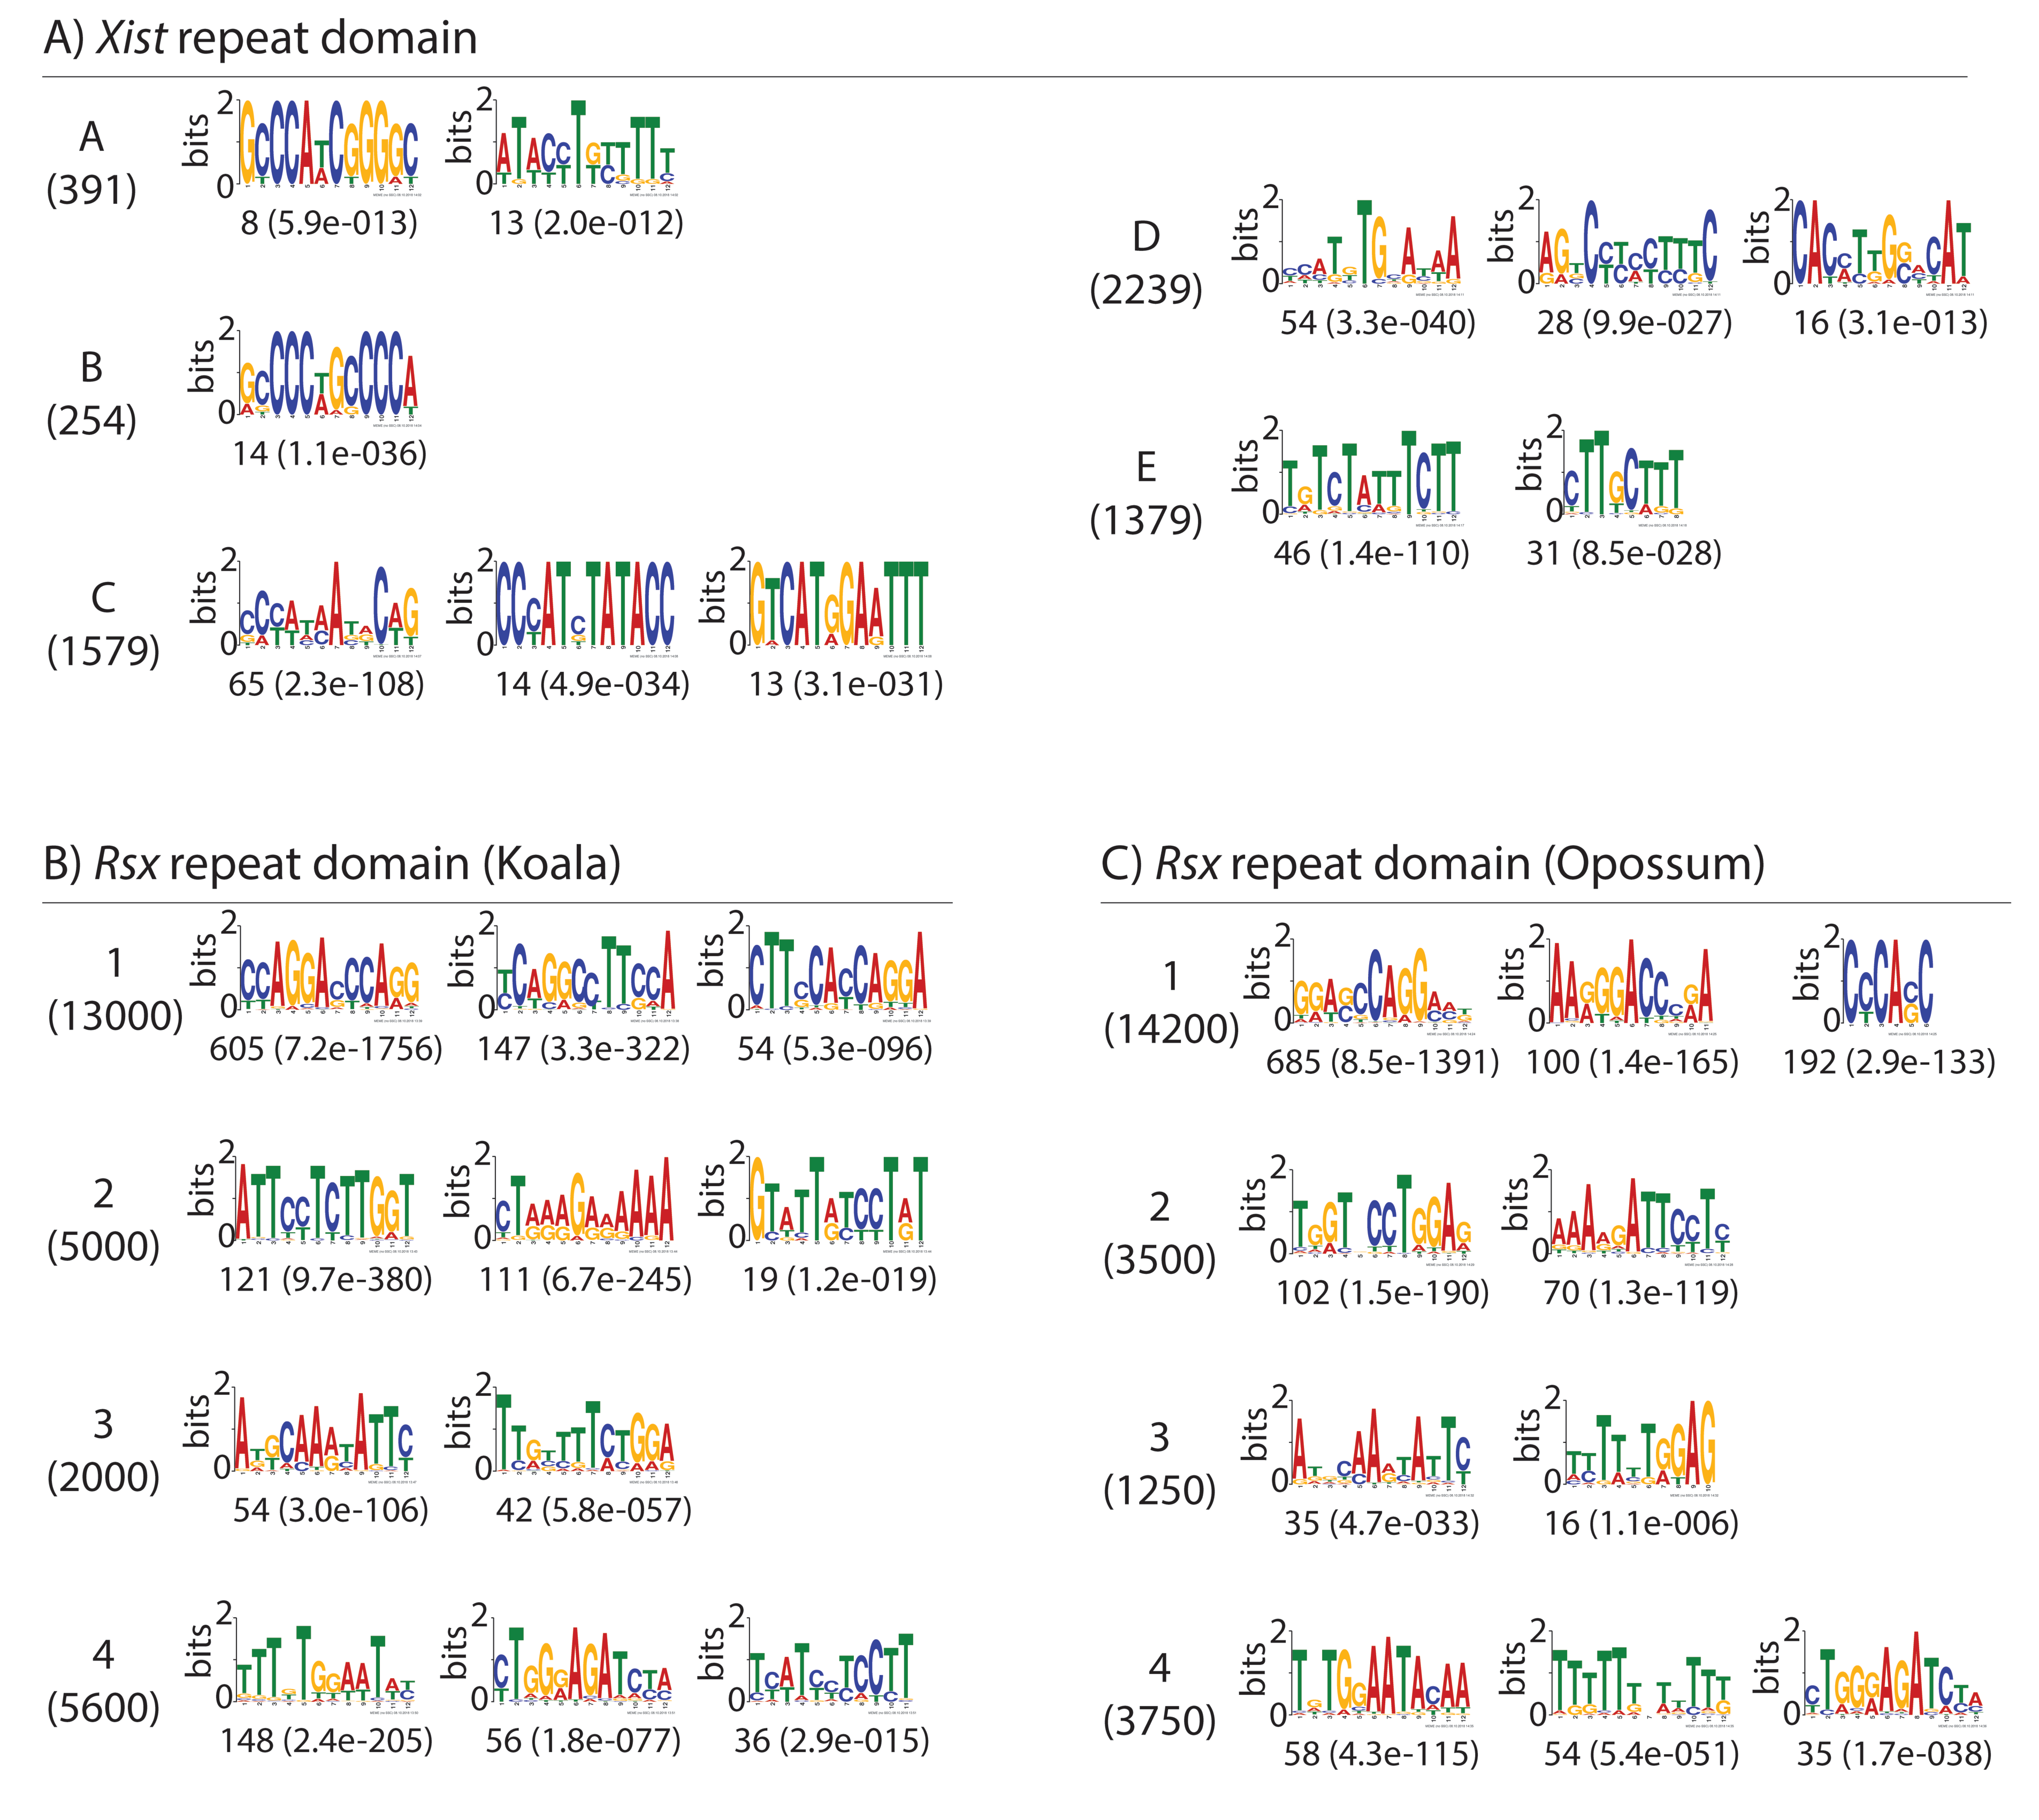
\includegraphics[angle=0, width=\textwidth]{images/fig3_v3-01.pdf}
\caption[Motif analysis of \emph{\emph{Xist}} and \emph{\emph{Rsx}}]{The top three de novo motifs identified by MEME in \emph{Xist} repeats (panel A; all repeats from mouse \emph{Xist} except for Repeat D, which is the human sequence), and in the four repeats in koala (B) and opossum (C) \emph{Rsx}. The length in nucleotides of each repeat is shown in parentheses below the repeat name. The number of matches to each motif, as well as the expectation-value for that number, is shown below each motif logo. Some repeats had less than three motifs detected by MEME.}
%\label{fig:x cubed graph}
\end{figure}
Similar to what we observed in our motif analysis (Figure 3), \emph{Rsx} Repeat 2 had the highest length-normalized abundance of polyA $k$-mers, followed closely by \emph{Rsx} Repeat 3 (Figure 4A). Repeat B, which is only ~250 nucleotides long and is almost entirely comprised of polyC sequence, had the highest length-normalized abundance of polyC $k$-mers, followed by \emph{Rsx} Repeat 1, and \emph{Xist} Repeats C, D, and A (Figure 4B). Mouse Repeat A had the highest length-normalized abundance of polyG $k$-mers, followed by \emph{Rsx} Repeats 1, 2, and 4 (Figure 4C). \emph{Xist} Repeats A and E, as well as \emph{Rsx} Repeats 3 and 4 had the highest length-normalized abundance of polyT $k$-mers, reflecting the high degree of SEEKR-detected similarity between these regions (Figure 4D). Similar trends were detected when we used $k$-mer lengths $k$ = 4, 5, and 6 for this analysis (Figure S3B). Thus, certain \emph{Xist} and \emph{Rsx} repeat domains share similarity in their overall $k$-mer profiles (Figure 2), in their enriched motifs (Figure 3), and in their enrichment in subsets of low-complexity $k$-mers that are comprised of mononucleotide runs (Figure 4). The repeat domains also harbor differences in sequence composition that are consistent with their lack of alignment via methods designed to detect linear sequence similarity (Figure 1).


\subsection{Enrichment of HNRNPK tandem repeat motifs in \emph{Xist} and \emph{Rsx}}
\emph{Xist} Repeat B is known to bind a protein called HNRNPK, and this binding activity is essential for \emph{Xist} to recruit PRC1 to the inactive X chromosome \cite{Pintacuda2017HnRNPKSilencing}. Given the quantitative and qualitative sequence similarities between \emph{Xist} Repeat B and \emph{Rsx} Repeat 1 (Figures 2 – 4), we sought to compare HNRNPK-binding potential between the two repeats using two conceptually distinct approaches. First, we weighted $z$-scores of individual $k$-mers in all \emph{Xist} and \emph{Rsx} repeat domains by the probability that the $k$-mer would occur in the Position-Weight-Matrix (PWM) describing the HNRNPK-binding motif from (\cite{Ray2013ARegulation}; see PWM in Figure 4E). We then summed HNRNPK-scaled $z$-scores over each repeat, and plotted the results in a manner similar to Figure 4A-D. In this analysis, a positive sum indicates that $k$-mers matching the HNRNPK PWM occur more frequently in the domain in question than they occur in other lncRNAs in the GENCODE database.

\begin{figure}[h!]
\centering
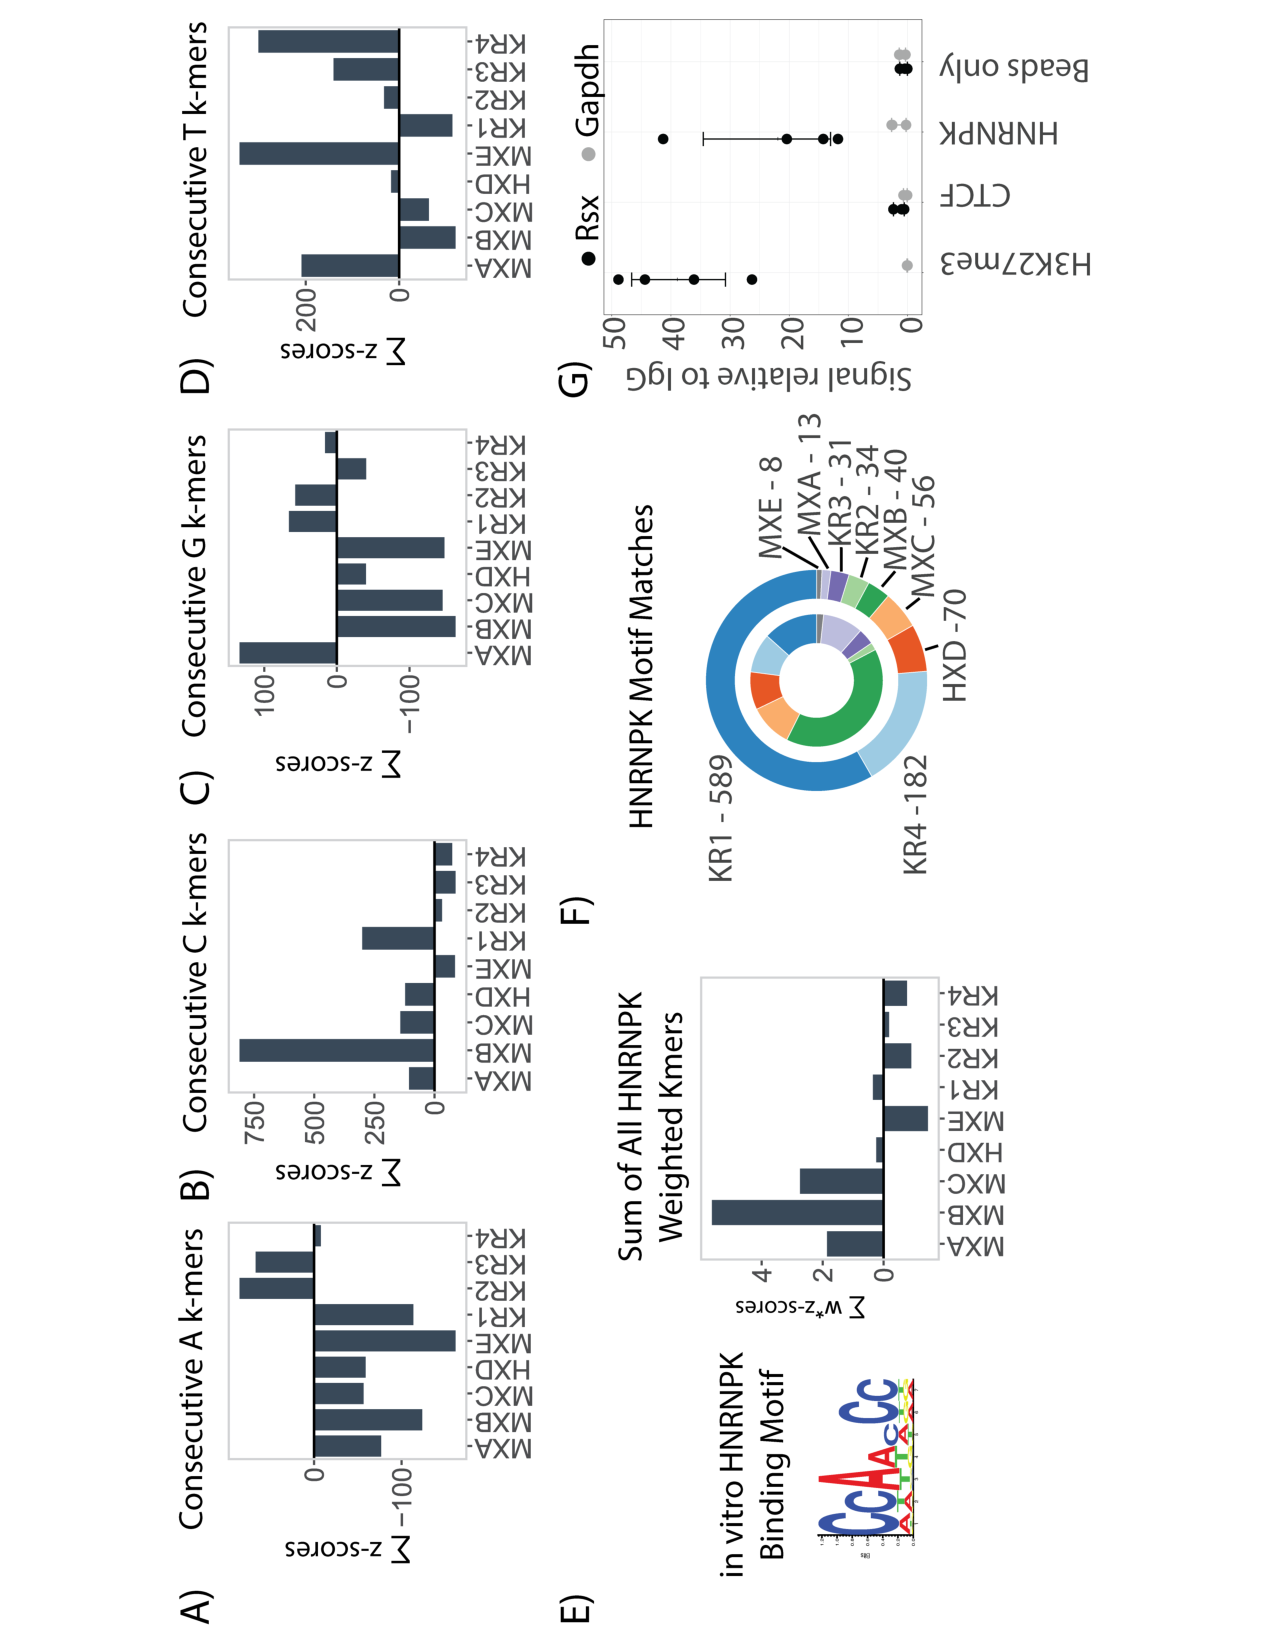
\includegraphics[angle=-90, width=.95\textwidth]{images/fig4_G-01.pdf}
\caption[Sequence and motif content in tandem repeats]{The sum of $z$-scores in each repeat for $k$-mers containing consecutive (A) A, (B) C, (C) G, and (D) T nucleotides. For this analysis we defined “consecutive” as at least two consecutive nucleotides of the specified identity, and used $k$-mer length k = 5 (Methods). Repeat abbreviations as in Figure 2. (E) The sum of $z$-scores for all $k$-mers in each \emph{Xist} and \emph{Rsx} repeat domain after weighting the $k$-mers by the likelihood with which they fit the consensus HNRNPK- binding motif. Motif logo that describes the consensus HNRNPK-binding motif obtained from (Ray et al., 2013) is also shown. (F) Component arcs of outer circle indicate the proportion and number of HNRNPK-binding motif matches detected by FIMO ($p<0.01$) in each \emph{Xist} and \emph{Rsx} repeat domain. Component arcs of inner circle indicate the proportion of motif matches in each repeat domain normalized for domain length. Repeat abbreviations as in Figure 2. (G) \emph{Rsx} enrichment relative to IgG control after RNA IP-qPCR in cultured fibroblasts from female M. domestica. For each antibody, left (black) is enrichment of \emph{Rsx}, right (grey) is enrichment of Gapdh. The histone modification H3K27me3 is enriched on the inactive X in marsupials, so an association with \emph{Rsx} was expected. CTCF has nanomolar affinity for RNA and along with “bead only”/no-antibody IP serves as a negative control demonstrating IP specificity \cite{Kung2015Locus-specificCTCF}. Dots represent values from replicate RNA IP experiments; error bars represent bootstrap 95 CI.}
%\label{fig:x cubed graph}
\end{figure}

On a length-normalized basis, \emph{Xist} Repeats B, C, A, and D, in descending order, had positive sums of HNRNPK-scaled $z$-scores. Repeat 1 was the only repeat in \emph{Rsx} to have a positive sum, perhaps consistent with a role in recruiting HNRNPK to \emph{Rsx} (Figure 4E). The sum of HNRNPK-scaled $z$-scores in \emph{Rsx} Repeat 1 was lower than the sums in \emph{Xist} Repeats B, C, and A (Figure 4E), which might be taken as evidence that on a length-normalized basis, \emph{Xist} Repeats B, C, and A have a higher density of $k$-mers that are likely to bind HNRNPK than \emph{Rsx} Repeat 1 or any other \emph{Rsx} repeat. However, at 13 kb in length, \emph{Rsx} Repeat 1 is $\approx$50 times longer than \emph{Xist} Repeat B, and is over half of the length of full-length \emph{Xist} itself \cite{Brockdorff10TheNucleus.,Brown10TheNucleus.,Johnson2018AdaptationGenome}. Thus, we also counted the absolute number of matches to HNRNPK-binding motifs in \emph{Xist} and \emph{Rsx} repeats. \emph{Rsx} Repeat 1 had 15 times more matches to HNRNPK-binding motifs than did \emph{Xist} Repeat B (589 matches in Repeat 1 compared to 40 matches in Repeat B; Figure 4F; \cite{Bailey2009MEMESearching}). \emph{Rsx} Repeat 4 also had a large number of matches to HNRNPK-binding motifs (182 matches), and human Repeat D and mouse Repeat C each had more HNRNPK-binding sites than Repeat B (70 and 56 matches, respectively, compared to 40 in Repeat B; Figure 4F). CLIP performed in mouse and human cells supports a direct association between HNRNPK and Repeat C and Repeat D, respectively (\cite{Cirillo2016QuantitativeEditor,VanNostrand2016RobusteCLIP}). Collectively, these data support the ideas that mouse Repeat C and human Repeat D cooperate with Repeat B in recruiting HNRNPK to \emph{Xist}, and suggest that \emph{Rsx} Repeat 1, and to a lesser extent, \emph{Rsx} Repeat 4, could also recruit HNRNPK to \emph{Rsx}. 

We next used RNA immunoprecipitation (RNA IP) followed by RT-qPCR to determine whether we could detect evidence of HNRNPK association with \emph{Rsx}. In fibroblast cells derived from a female gray short-tailed opossum, Monodelphis domestica, we found that HNRNPK IP enriched for \emph{Rsx} 20-fold over IgG control IPs (Figure 4G). This enrichment was similar to that seen for an IP using an antibody that detects histone H3-lysine27-trimethylation (H3K27me3), a modification known to be enriched on the opossum inactive X (Figure 4G; (Wang et al., 2014)). Gapdh mRNA was not enriched by IP of HNRNPK or H3K27me3 (Figure 4G). IP of CTCF, a protein that binds RNA with nanomolar affinity in a sequence non-specific manner, showed neither \emph{Rsx} nor Gapdh enrichment (Figure 4G; \cite{Kung2015Locus-specificCTCF}). Leaving out HNRNPK antibody prior to performing IP and qPCR also led to a loss of \emph{Rsx} signal (“beads only” in Figure 4G). DNase-treated input RNA (no reverse transcription control) did not yield signal in qPCR assays, indicating DNase digestion prior to cDNA synthesis and qPCR proceeded to completion (not shown). These data support our computational analyses and suggest that HNRNPK associates with \emph{Rsx} in marsupial cells.

\subsection{Conservation of \emph{Xist} and \emph{Rsx} Repeats}
Considering that not all of the repeat domains in \emph{Xist} exhibit conservation across eutherian mammals, we sought to determine whether or not the repeat domains in koala \emph{Rsx} were conserved in another marsupial. \emph{Rsx} was originally identified in opossum \cite{Grant2012RsxInactivation}, but the most current assembly of the opossum genome (mondom5) harbors significant gaps within the sequence of \emph{Rsx}. 

To assemble a complete sequence of opossum \emph{Rsx} for comparison to koala, we used Oxford Nanopore technology to sequence two Bacterial Artificial Chromosomes (BACs) that encompassed the opossum \emph{Rsx} locus (VMRC18-839J22 and VMRC18-303M7). De novo assembly and polishing of sequence reads identified a single 235,139 base contig aligning to chrX that had on average a 0.5\% error rate with the mondom5 assembly (File S3). Our assembly filled in 16620 bases of unannotated sequence in the \emph{Rsx} locus, 361 bases of which were a part of the spliced \emph{Rsx} lncRNA annotation from \cite{Grant2012RsxInactivation}.

\begin{figure}[h!]
\centering
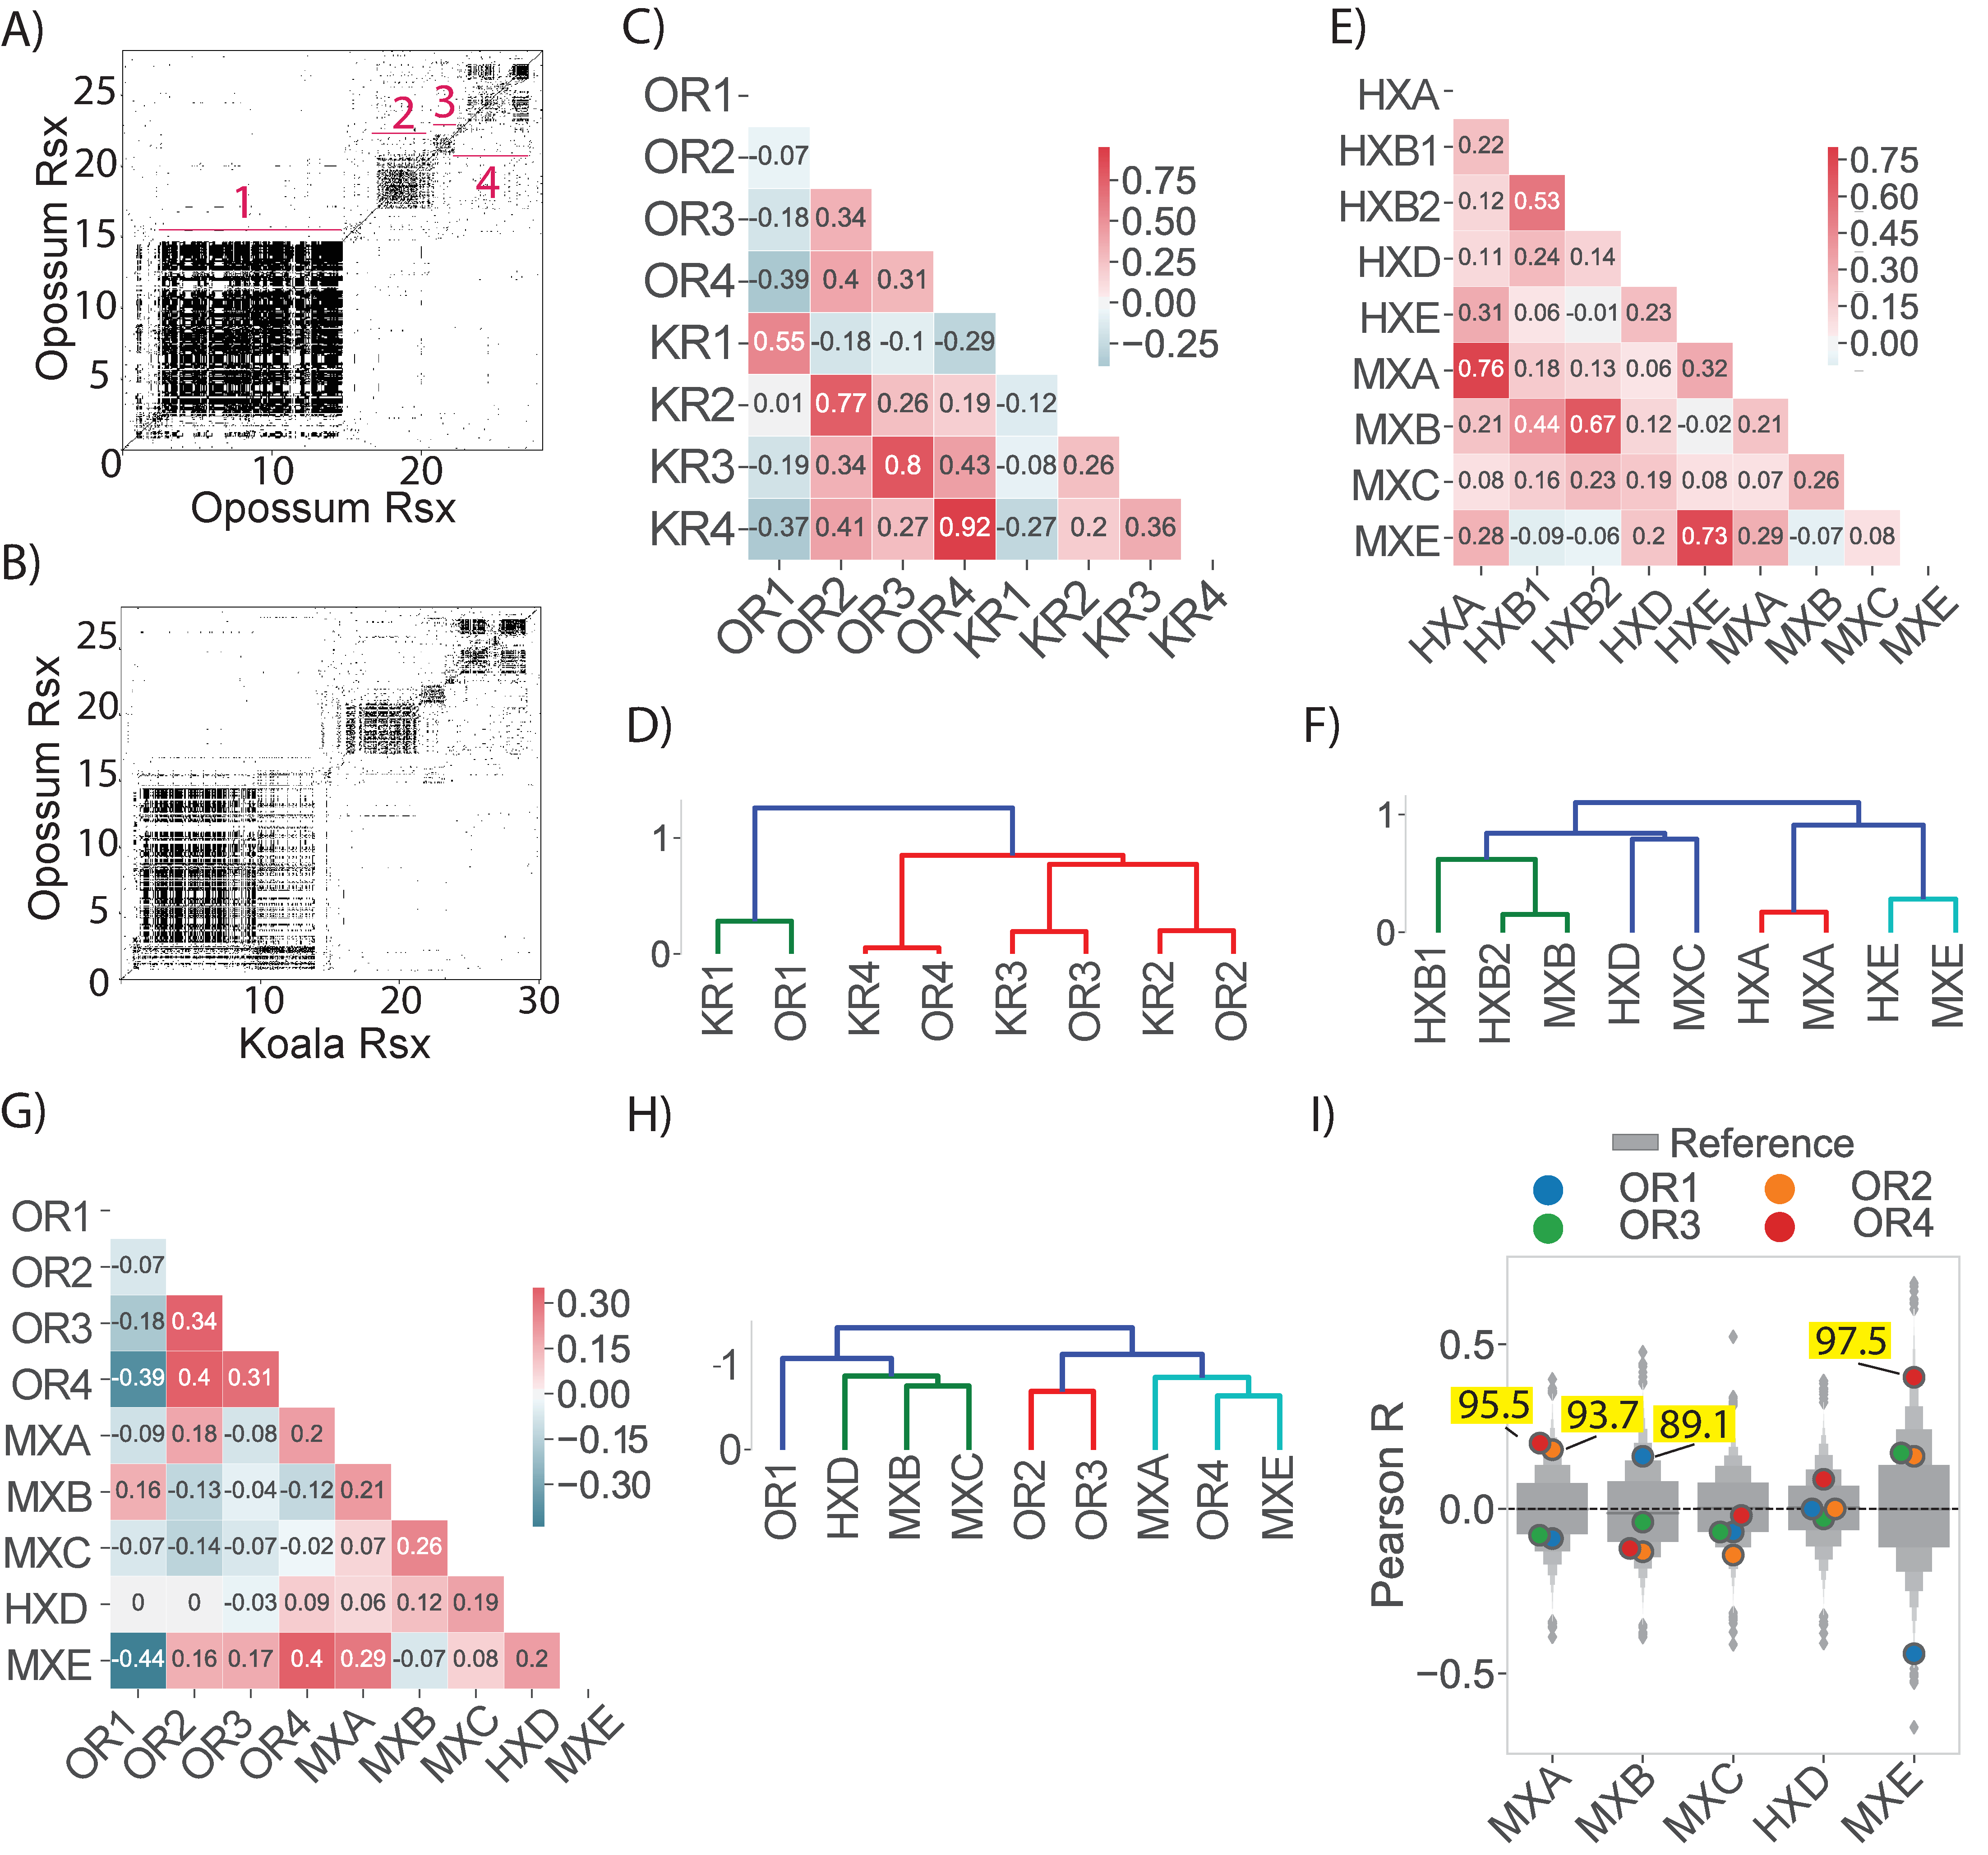
\includegraphics[ width=.95\textwidth]{images/fig5.pdf}
\caption[\emph{Rsx} repeat domains are conserved between koala and opossum.]{(A,B) Dot plots of opossum \emph{Rsx} aligned to (A) itself or (B) koala \emph{Rsx}. (C) Similarity between repeat domains in koala and opossum \emph{Rsx} as calculated in Figure 2C. (D) Hierarchical cluster of similarity values from (C). (E) Similarity between repeat domains in mouse and human \emph{Xist} as calculated in Figure 2C. (F) Hierarchical clustering of similarity values from (E). G) Similarity between repeat domains in opossum \emph{Rsx} and \emph{Xist} repeat domains as calculated in Figure 2C. (H) Hierarchical cluster of similarity values from (G). (I) Percentiles for Pearson’s R for opossum \emph{Rsx} repeat domains compared to each \emph{Xist} repeat domain as in Figure 2D. Numbers mentioned in the body of the manuscript are highlighted in yellow.}
\label{fig:5}
\end{figure}

Alignment of this ungapped assembly of spliced opossum \emph{Rsx} to koala \emph{Rsx} revealed high levels of similarity between their repeat domains in a dot plot analysis (Figure 5A, B). This similarity could also be seen at the level of $k$-mers (Figure 5C, D), and by extraction of enriched motifs using MEME (Figure 3B, C). Opossum and koala, which are members of distantly related American and Australian marsupial families, respectively, diverged approximately 82 million years ago \cite{Kumar2017TimeTree:Times}. By comparison, mouse and human are separated by approximately 90 million years of evolution \cite{Kumar2017TimeTree:Times}. Repeat domains 1 through 4 in opossum and koala \emph{Rsx} exhibited levels of sequence similarity that approximated or exceeded the similarity found between the repeat domains in mouse and human \emph{Xist} (with the exception of Repeat C/Repeat D; Figure 5C-F). Thus, the repeat domains in \emph{Rsx} appear to be at least as conserved between distantly related marsupials as the repeat domains in \emph{Xist} are conserved among eutherians.

Next, we compared the $k$-mer contents of repeat domains in \emph{Xist} to the $k$-mer contents of repeat domains in opossum \emph{Rsx}. We identified a level of similarity (Figure 5G, H, I) that mirrored the similarity we found between repeat domains in \emph{Xist} and koala \emph{Rsx} (Figure 2B, D, E). \emph{Xist} Repeat A was most similar to opossum Repeats 2 and 4 ($93.7^{th}$ and $95.5^{th}$ percentile relative to all other mouse lncRNAs, respectively); \emph{Xist} Repeat B was most similar to opossum Repeat 1 (89.1$^{st}$ percentile relative to all other lncRNAs); and \emph{Xist} Repeat E was most similar to opossum Repeat 4 ($97.5^{th}$ percentile relative to all other lncRNAs; Figure 5I). Thus, the major repeat domains in \emph{Rsx} are conserved between opossum and koala, and the repeat domains in \emph{Rsx} from both marsupials harbor $k$-mer contents similar those in repeat domains from mouse and human \emph{Xist}.

\subsection{Multiple protein-binding motifs are enriched to extreme levels in \emph{Xist} and \emph{Rsx} repeat domains}
We examined the extent to which \emph{Xist} and \emph{Rsx} repeat domains were enriched for sequence motifs known to recruit RNA binding proteins, hypothesizing that the patterns of enrichment might provide additional insight into similarities between the two lncRNAs. For this analysis, we downloaded PWMs for all mammalian RNA binding proteins available in the CISBP-RNA database \cite{Ray2013ARegulation}, and for each PWM in each repeat, we quantified enrichment by weighting $k$-mer $z$-scores by the probability that the $k$-mer matched the PWM, then calculating the sum of those weights, as we did for the HNRNPK PWM in Figure 4E. To gauge the extent of enrichment relative to other mouse lncRNAs, we determined the percentile rank of the sum for each PWM in each repeat relative to the sums generated from the same PWM-weighting procedure performed on all mouse lncRNAs. We then hierarchically clustered repeat domains from \emph{Xist} and \emph{Rsx} based on the percentile ranks of motif enrichment for each domain. The results of these analyses are shown in Figure 6A.

\begin{figure}[h!]
\centering
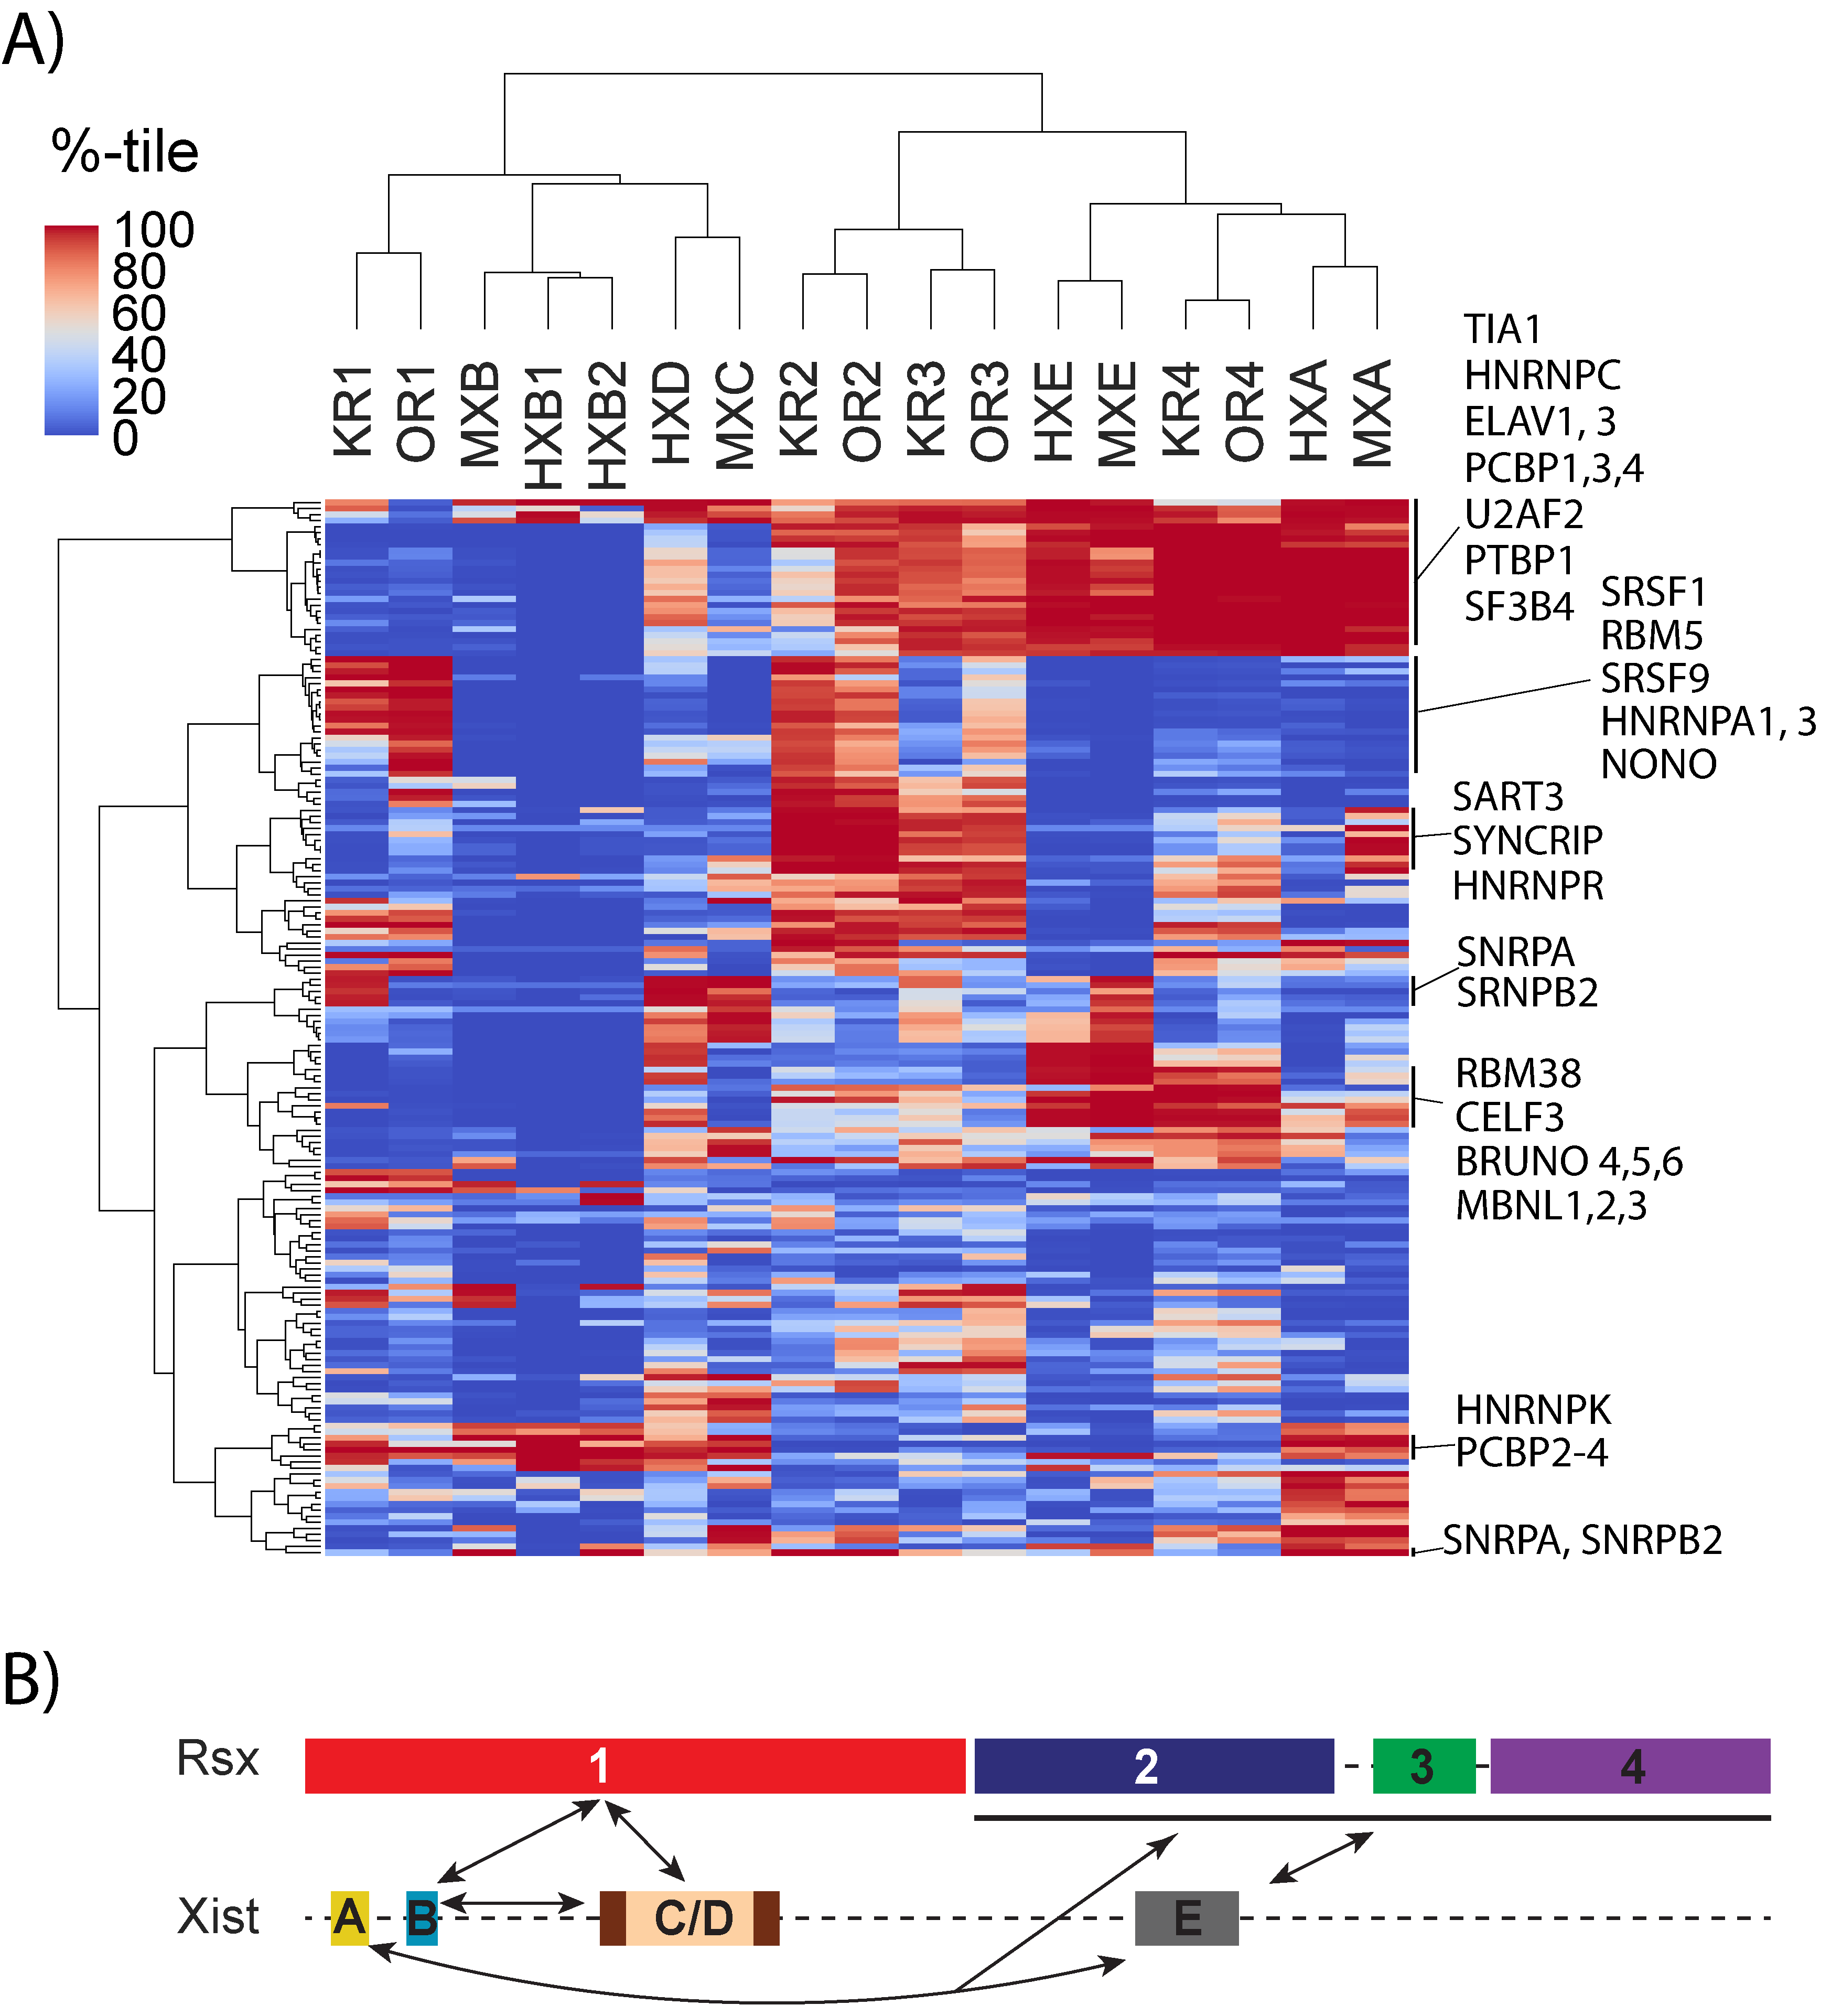
\includegraphics[width=.95\textwidth]{images/fig6.pdf}
\caption[Protein-binding motif enrichment in repeats of \emph{Xist} and \emph{Rsx}, and similarity model.]{(A) Hierarchically clustered heatmap of PWM weighted $z$-scores for each repeat in \emph{Xist} and \emph{Rsx}, expressed as a percentile relative to the set of all GENCODE M18 lncRNA annotations. (B) Regions predicted to have similar protein-binding functions in \emph{Xist} and \emph{Rsx}. Arrows connect domains in each lncRNA that have similar $k$-mer and motif contents.}
\label{fig:6}
\end{figure}

Using ranked enrichment of protein-binding motifs as a metric for hierarchical clustering, we  identified the same relationships between \emph{Xist} and \emph{Rsx} repeat domains as we did when we hierarchically clustered domains by their $k$-mer content alone (dendrogram in Figure 6A compared to dendrograms in Figures 2E and 5H). Via protein-binding motif enrichment, \emph{Xist} Repeats B, C, and D formed a second order cluster that next joined with \emph{Rsx} Repeat 1.  This clustering order is the same as that detected using $k$-mer content alone (Figure 6A vs. 2E and 5H). Likewise, protein-binding motif enrichment grouped Repeats A and E together with \emph{Rsx} Repeat 4, while \emph{Rsx} Repeats 2 and 3 formed a separate cluster that joined with the Repeat-A-E-4 cluster. Again, similar clustering patterns were obtained based purely on $k$-mer content (Figure 6A vs. 2E and 5H). We note that the motifs used to create these clusters are limited in complexity and are capable of recruiting different proteins depending on cellular and sequence contexts \cite{Dominguez2018SequenceProteins,Ray2013ARegulation}. Thus, the enrichment of a particular protein-binding motif in an individual \emph{Xist} or \emph{Rsx} repeat domain does not provide direct evidence that the protein binds to the domain. Nevertheless, these results are consistent with the notions that lncRNA $k$-mer content encodes information about protein-binding potential \cite{Kirk2018FunctionalContent}, and that the various repeats in \emph{Xist} and \emph{Rsx} encode function through the concerted recruitment of multiple RNA-binding proteins.

A closer inspection of the protein-binding motifs that were enriched in each repeat domain yielded several insights. First, our motif analysis uncovered relationships between repeat domains that were not obvious from direct $k$-mer comparisons. For example, both human and mouse \emph{Xist} Repeat B were enriched in motifs that recruit polyC-binding proteins and little else (Figure 6A; Table S4). \emph{Rsx} Repeat 1, which most closely resembles \emph{Xist} Repeat B at the level of $k$-mers, was also enriched in polyC-binding motifs, in both koala and opossum (Figure 6A; Table S4). However, Repeat 1 from koala and opossum \emph{Rsx} were also enriched in many motifs that were absent in Repeat B, such as motifs that bind the proteins SRSF1, SRSF9, and RBM5 (Figure 6A; Table S4). In addition, while both pure $k$-mer analysis and motif analysis identified similarities between \emph{Xist} Repeats A and E and \emph{Rsx} Repeats 2, 3, and 4, our motif analysis also identified similarities exclusive to pairs of domains within this group, such as similarities between \emph{Rsx} Repeats 2 and 3 and similarities between \emph{Xist} Repeat E and \emph{Rsx} Repeat 4 (Figure 6A; Table S4). 

Second, within individual repeat domains, many protein-binding motifs were enriched to extreme levels. Well over half of the motifs analyzed (101 out of 175) were in the $99^{th}$ percentile in terms of their enrichment relative to other mouse lncRNAs in at least one \emph{Xist} or \emph{Rsx} repeat domain, and all repeat domains in \emph{Xist} and \emph{Rsx} harbored multiple protein-binding motifs that were enriched at the $99^{th}$ percentile or greater (Figure 6A; Table S4). This extremity was notable considering that most \emph{Xist} and \emph{Rsx} repeats are greater in length than the average mouse lncRNA (Figure 2A). For example, at 13kb in length, \emph{Rsx} Repeat 1 is longer than 99.97\% of spliced mouse lncRNAs (Figure 2A). Nevertheless, on a length-normalized basis, multiple protein-binding motifs were enriched in Repeat 1 at the $99^{th}$ percentile, in both koala and opossum \emph{Rsx}. Inasmuch as motif density is known to be an important driver of associations between proteins and RNA \cite{Dominguez2018SequenceProteins,Kirk2018FunctionalContent,VanNostrand2016RobusteCLIP}, our data suggest that at the level of sequence composition, the repeat domains in \emph{Xist} and \emph{Rsx} each have the potential to serve as high-affinity binding platforms for multiple proteins.

Lastly, many of the most strongly enriched motifs in both \emph{Xist} and \emph{Rsx} are known to recruit near-ubiquitous RNA-binding proteins that play core roles in the process of splicing \cite{Wahl2015Snapshot:I}. These included PTBP1, RMB5, SF3B4, SNRPA, SNRPB2, U2AF2, multiple SR proteins, and multiple HNRNP proteins, including HNRNPA1, HNRNPC, and HNRNPK (Figure 6A; Table S4). We recognize that the motifs available for this analysis are biased towards RNA-binding proteins whose functions are best understood; overwhelmingly, these proteins are splicing factors \cite{Dominguez2018SequenceProteins,Ray2013ARegulation}. Nevertheless, it is possible that an extreme enrichment for a motif that recruits a ubiquitously expressed splicing factor may confer a function that a single binding motif would not. For example, we presume that the function of Repeat B could not be recapitulated by a single motif that binds HNRNPK \cite{Pintacuda2017HnRNPKSilencing}. 


\section{Discussion}
\emph{Xist} has served as a paradigmatic regulatory lncRNA for more than 25 years \cite{Brockdorff2018LocalNcRNA,Balaton2018TheChromosome,DaRocha2017NovelConformation,Sahakyan2018TheCompensation}. Nevertheless, it has been challenging to apply the information gained from the study of \emph{Xist} to other lncRNAs. This is because \emph{Xist} has little linear sequence similarity to other RNAs, even to lncRNAs like \emph{Rsx}, which seem likely to encode analogous functions \cite{Grant2012RsxInactivation,Wang2014Chromosome-wideDomestica}. In the present study, we used a non-linear method of sequence comparison called SEEKR \cite{Kirk2018FunctionalContent} to compare the repetitive regions of \emph{Xist} and \emph{Rsx}. Our data provide sequence-based evidence to support the hypothesis that \emph{Xist} and \emph{Rsx} are functional analogues that arose through convergent evolution, and provide insights into mechanisms through which their repeat domains may encode function. 

Unexpectedly, at the level of $k$-mers, the repeat domains of \emph{Xist} and \emph{Rsx} partitioned into two major clusters. \emph{Xist} Repeats B, C, and D were highly similar to each other and to \emph{Rsx} Repeat 1, whereas \emph{Xist} Repeats A and E were most similar to each other and to \emph{Rsx} Repeats 2, 3, and 4. From prior analyses of sequence content, there is little that would have suggested that the repeats in these two lncRNAs would cluster together in such a manner. However, prior molecular analyses of \emph{Xist} are consistent with such a clustering \cite{Brockdorff2018LocalNcRNA,Balaton2018TheChromosome,DaRocha2017NovelConformation,Sahakyan2018TheCompensation}. 

Specifically, \emph{Xist} Repeats B and C are known to play important roles in recruiting PRC1 to the inactive X through their ability to bind HNRNPK and possibly other proteins \cite{Pintacuda2017HnRNPKSilencing}. The similarity between Repeats B and C and \emph{Xist} Repeat D and \emph{Rsx} Repeat 1 suggests that the latter two repeats may also play roles in recruiting PRC1. Consistent with this possibility, we found that an antibody specific to HNRNPK robustly retrieved \emph{Rsx} RNA in an IP. Moreover, eCLIP data show that \emph{Xist} Repeat D is enriched for HNRNPK binding in human cells (\cite{VanNostrand2016RobusteCLIP}). Thus, even within \emph{Xist}, murid and non-murid mammals may have convergently evolved separate repeats to recruit PRC1, in the form of Repeats C and D, respectively.

Relatedly, \emph{Xist} Repeats A and E have been implicated in recruitment of PRC2 to the inactive X, both via direct and cooperative means \cite{Almeida2017PCGF3/5-PRC1Inactivation,Cifuentes-Rojas2014Regulatory2,Davidovich2015TowardRNA,Kohlmaier2004AInactivation,Ridings-Figueroa2017TheTerritory,Sunwoo2017RepeatCIZ1,Wang2017TargetingGuanines,Zhao2008PolycombChromosome}. The similarity between \emph{Xist} Repeats A and E and \emph{Rsx} Repeats 2, 3, and 4 suggests that the \emph{Rsx} repeats could also play roles in recruiting PRC2. 

Based on these data, we propose that the two major clusters of repeats in \emph{Xist} and \emph{Rsx} function in part to cooperatively recruit PRC1 and PRC2 to chromatin. Within \emph{Xist}, Repeat B plays a dominant role in recruiting PRC1 via its ability to bind HNRNPK; in turn, PRC1-induced chromatin modifications likely stimulate loading of PRC2 onto chromatin of the inactive X \cite{Almeida2017PCGF3/5-PRC1Inactivation,Pintacuda2017HnRNPKSilencing}. Nevertheless, a PRC1-dominant model does not preclude other repeats in \emph{Xist} or \emph{Rsx} from functioning in PRC2 recruitment. Indeed, while there does not appear to be a single domain in \emph{Xist} that is absolutely required to recruit PRC2 during the early stages of XCI \cite{Kohlmaier2004AInactivation,Wutz2002ChromosomalRNA}, it is possible that multiple domains in \emph{Xist} recruit PRC2 duplicatively, such that deletion of any single domain alone does not cause complete loss in PRC2 recruitment. This hypothesis is supported by prior studies that link both Repeat A and E to recruitment of PRC2 \cite{Almeida2017PCGF3/5-PRC1Inactivation,Cifuentes-Rojas2014Regulatory2,Davidovich2015TowardRNA,Kohlmaier2004AInactivation,Ridings-Figueroa2017TheTerritory,Sunwoo2017RepeatCIZ1,Wang2017TargetingGuanines,Zhao2008PolycombChromosome}, and by our own data that show \emph{Xist} Repeats A and E and \emph{Rsx} Repeats 2, 3, and 4 have similar $k$-mer profiles and motif contents. PRC1, PRC2, and related complexes function cooperatively in flies, mammals, and plants \cite{Blackledge2015TargetingStory,Li2018Polycomb-mediatedPlants,Schuettengruber2014CooperativityDrosophila}. Considering this cooperativity, it is conceivable that the repeat domains in \emph{Xist} and \emph{Rsx} also cooperate to distribute PRC1 and PRC2 on chromatin.

Beyond recruiting PRCs, \emph{Xist} evades nuclear export, it associates with transcribed regions of chromatin, and it induces Polycomb-independent gene silencing \cite{Balaton2018TheChromosome,Brockdorff2018LocalNcRNA,Sahakyan2018TheCompensation}. It is possible that \emph{Rsx} carries out many, if not all of these actions, and that \emph{Rsx} relies on sets of proteins similar to those employed by \emph{Xist} to achieve them \cite{Grant2012RsxInactivation,Wang2014Chromosome-wideDomestica}. We found that all \emph{Xist} and \emph{Rsx} repeat domains harbored extreme levels of enrichment for multiple motifs known to recruit different subsets of RNA-binding proteins. Most of these proteins have been best-characterized in the context of splicing, rather than epigenetic silencing.

In light of these data, we suggest that the repeat domains in \emph{Xist} and \emph{Rsx} may encode some of their functions not by recruiting a set of dedicated RNA silencing factors, but by engaging with ubiquitously-expressed RNA-binding proteins in ways that are distinct from most other RNAs. Such a model was recently proposed \cite{Brockdorff2018LocalNcRNA}, and agrees well with what is known about the specificity of RNA-protein interactions. Most RNA-binding proteins have limited sequence specificity, and are capable of binding many thousands of regions in hundreds to thousands of expressed RNAs \cite{Dominguez2018SequenceProteins,Ray2013ARegulation,VanNostrand2016RobusteCLIP}. SPEN and HNRNPK are two RNA-binding proteins that are critical for \emph{Xist}-induced silencing, yet they clearly associate with RNAs other than \emph{Xist} \cite{Cirillo2016QuantitativeEditor,VanNostrand2016RobusteCLIP}. Relatedly, many other proteins important for \emph{Xist}-induced silencing play central roles in RNA splicing and nuclear export and, through these latter roles, likely associate with a large portion of the transcriptome \cite{Moindrot2015ASilencing}. Thus, \emph{Xist} and \emph{Rsx} may distinguish themselves from other chromatin-associated transcripts not necessarily by the proteins to which they bind, but by the manner in which they bind these proteins.

That the related repeat domains were present in a different order in \emph{Xist} and \emph{Rsx} supports the notion that within a lncRNA, the order of functional domains is likely to be less important than the presence of the functional domains (Figure 6B). This notion is consistent with a body of work that suggests lncRNAs encode regulatory function in a modular fashion, via discrete domains that recruit distinct subsets of effector proteins \cite{Hacisuleyman2016FunctionLocus,Hezroni2015PrinciplesSpecies,Johnson2014TheRNAs,Kelley2014TransposableInteractions,Kirk2018FunctionalContent,Liu2017VisualizingRepA,Lu2016RNAStructure,Lubelsky2018SequencesCells,Patil2016M6Repression,Pintacuda2017HnRNPKSilencing, Smola2016SHAPECells,Somarowthu2015HOTAIRStructure,Tsai2010LongComplexes, Wutz2002ChromosomalRNA}.

From a methodological standpoint, our manuscript outlines approaches that should prove useful in the study of functional domains in other sets of RNAs. Intuitively, $k$-mer based comparisons like SEEKR seem most likely to succeed in identifying similarity when the domains of interest are repetitive. By nature, repetitive domains that share enrichments of similar subsets of $k$-mers will be more similar to each other than they will be similar to the average non-repetitive region in the transcriptome. 

Nevertheless, similarity between two repetitive domains, when observed, should be carefully considered, especially when the similarity occurs in lncRNAs such as \emph{Xist} and \emph{Rsx}, which are expressed at similar levels in equivalent subcellular compartments \cite{Grant2012RsxInactivation,Wang2014Chromosome-wideDomestica}. Motif density is known to be a dominant factor driving protein/RNA interactions \cite{Dominguez2018SequenceProteins,Kirk2018FunctionalContent,Wang2014Chromosome-wideDomestica}. All other variables being equal, two lncRNAs that harbor domain-specific $k$-mer similarity should possess similar protein-binding profiles that could specify similar or analogous function. 

However, SEEKR is not limited to analysis of repetitive domains. It also has the ability to detect similarity between repetitive and non-repetitive domains and between strictly non-repetitive domains as well. In any given sequence, a set of $k$-mers can be arranged in repetitive or non-repetitive ways, and SEEKR has no inherent preference for one over the other. As a contrived example, the sequence of \emph{Xist} Repeat D can be shuffled in a way that eliminates its repeated monomers, yet entirely preserves its $k$-mer content (File S1). By BLAST, this shuffled sequence has little internal similarity to itself or to Repeat D (Figure S6). Yet, by $k$-mer content, the shuffled sequence and Repeat D are literally identical (Figure S6). In a real-world example, the top five lncRNAs that SEEKR found to be the most similar to Repeat D are not nearly as repetitive as Repeat D itself (Figure S6). Of all \emph{Xist} and \emph{Rsx} repeats, Repeat D is the most complex (Figure 2B). Nevertheless, these results demonstrate that $k$-mer based similarity searches performed with repetitive domains can identify non-repetitive top hits.

With regard to non-repetitive domains, our 2018 study showed that SEEKR rivaled BLAST-like alignment in its ability to detect lncRNA homologues in human and mouse  \cite{Kirk2018FunctionalContent}. The majority of homologues detected by SEEKR either lacked obvious repetitive elements, or were predominantly comprised of non-repetitive sequence; the lncRNAs H19, Hottip, Malat1, Miat, and RMST being specific examples. We also found that SEEKR could identify \emph{Xist}-like repressive activity in several synthetic and natural lncRNAs that lacked repetitive elements \cite{Kirk2018FunctionalContent}. Thus, even in non-repetitive regions of RNA, SEEKR should be capable of detecting meaningful similarities. However, functional domains comprised of high-complexity sequence elements will likely remain challenging to identify, regardless of the method in use.

Key variables to decide upon when using SEEKR are the $k$-mer length and the appropriate set of RNAs that define the background $k$-mer frequency; i.e. the set of RNAs used to define the means and standard deviations from which $k$-mer $z$-scores are calculated. At present, data regarding functional domains in lncRNAs are too limited to arrive at conclusive recommendations for either variable. We favor using a $k$-mer length at which 4$^$k most closely resembles the length of the shortest domain being analyzed. This approach minimizes the number of $k$-mers that yield counts of zero in the domain. Data from the present study as well as our prior work suggest that this minimization increases discriminatory power ( \cite{Kirk2018FunctionalContent}). 

In terms of the set of RNAs that should be used to define the background $k$-mer frequency, it is worth noting that SEEKR measures relative, not absolute, similarity. Pearson’s r values returned by SEEKR reflect the similarity between two sequences relative to the $k$-mer frequency present in the background set of RNAs. We have found that using a background set of all lncRNAs in a genome provides a convenient way to identify trends. For example, in the present study, we used all known spliced lncRNAs in the mouse as a background set. Accordingly, we were able to identify properties in the repeat domains of \emph{Xist} and \emph{Rsx} that were distinct from the average spliced lncRNA annotated by GENCODE \cite{Derrien2012TheExpression}.

In our initial description of SEEKR, we used $k$-mer contents of full-length lncRNAs as search features; we did not examine $k$-mer contents at the level of individual domains \cite{Kirk2018FunctionalContent}. The domain-centric approaches outlined in the present study may be better suited for lncRNAs such as \emph{Xist} and \emph{Rsx}, which have multiple functions that are likely to be distributed amongst multiple domains. Indeed, at the level of $k$-mers, full-length \emph{Xist} and \emph{Rsx} were negatively correlated to each other. Similarities between the two lncRNAs emerged only when we took a domain-centric approach. Other eutherian lncRNAs known to harbor \emph{Xist}-like silencing function, such as Kcnq1ot1 and Airn, are exceptionally long – each on the order of 90kb. Extrapolating from our findings above, we would expect these lncRNAs to harbor the greatest levels of similarity to each other not at the level of their full-length transcripts, but at the level of specific domains.

\section{Methods}
\subsection{Long read sequencing of \emph{Rsx}}
High molecular weight DNA from VMRC18-839J22 and VMRC18-303M7 BACs was prepared using the NucleoBond BAC 100 kit (Machery Nagel). DNA from the two BAC preparations was pooled, sheared to an average length of 20kb using a g-TUBE (Covaris), and then sequenced on the Oxford Nanopore Technologies (ONT) MinION using an R9.4 flow cell (FLO-MIN106) following the 1D ligation protocol (SQ$k$-LSK109). 

Reads were base-called with Albacore 2.3.1 (ONT) then assembled using Flye 2.3.5b \cite{Kolmogorov2019AssemblyGraphs}. The six resulting scaffolds were aligned to E. coli K12 (NC$_$000913.3), opossum chromosome X (MonDom5, NC$_$008809.1) and the pCC1BAC cloning vector (EU140750.1). Scaffolds consisting entirely of E. coli or cloning vector DNA were removed. Three scaffolds aligned to adjacent regions of the MonDom5 X chromosome. These were merged together into a single candidate assembly sequence that was then polished iteratively with Racon 1.3.2 four times \cite{Vaser2017FastReads}, followed by Nanopolish 0.10.1 \cite{Loman2015AData}, to produce a final complete assembly of 235,139 nucleotides.

This polished assembly sequence was aligned again to MonDom5 using BLASTN to establish start and end coordinates to use as a reference when replacing the gaps in MonDom5 with the completed sequence in our assembly. The final sequence of opossum \emph{Rsx} used in this work was generated using splice annotations from \cite{Grant2012RsxInactivation}, and replacing the N’s in mondom5 with the corresponding sequence from our polished assembly (nucleotide substitutions are listed in Table S3). Raw sequencing reads were deposited in NCBI’s SRA, under accession number PRJNA522427.

\subsection{Nanopore sequencing and \emph{\emph{Rsx}} splice structure determination}
High molecular weight DNA from VMRC18-839J22 and VMRC18-303M7 BACs was prepared
using the NucleoBond BAC 100 kit (Machery Nagel). DNA from the two BAC preparations was pooled, sheared to an average length of 20kb using a g-TUBE (Covaris), and then sequenced on the Oxford Nanopore Technologies (ONT) MinION using an R9.4 flow cell (FLO-MIN106) following the 1D ligation protocol (SQ$k$-LSK109).
Reads were base-called with Albacore 2.3.1 (ONT) then assembled using Flye 2.3.5b \cite{Kolmogorov2019AssemblyGraphs}. The six resulting scaffolds were aligned to E. coli K12 (NC$_$000913.3), opossum chromosome X (MonDom5, NC$_$008809.1) and the pCC1BAC cloning vector (EU140750.1). Scaffolds consisting entirely of E. coli or cloning vector DNA were removed. Three scaffolds aligned to adjacent regions of the MonDom5 X chromosome. These were merged together into a single candidate assembly sequence that was then polished iteratively with Racon 1.3.2 four times \cite{Vaser2017FastReads}, followed by Nanopolish 0.10.1 \cite{Loman2015AData}, to produce a final complete assembly of 235,139 nucleotides.

This polished assembly sequence was aligned again to MonDom5 using BLASTN to establish start and end coordinates to use as a reference when replacing the gaps in MonDom5 with the completed sequence in our assembly. The final sequence of opossum \emph{Rsx} used in this work was generated using splice annotations from \cite{Grant2012RsxInactivation}, and replacing the N’s in mondom5 with the corresponding sequence from our polished assembly. Raw sequencing reads were deposited in NCBI’s SRA, under accession number PRJNA522427.

\subsection{Defining tandem repeat domains of \emph{\emph{Xist}/\emph{Rsx}}}
The sequence of all \emph{Xist} and \emph{Rsx} repeat domains used in this work can be found in File S1. The sequences of all full-length \emph{Xist} and \emph{Rsx} lncRNAs used in this work can be found in File S2. The spliced mouse \emph{Xist} sequence was sourced from the mm10 build of the mouse genome and annotations for the tandem repeats were sourced from \cite{Brockdorff10TheNucleus.}. The spliced human \emph{Xist} sequence was sourced from the hg38 build of the human genome and the annotations for the tandem repeats were sourced from \cite{Brown10TheNucleus.,Yen2007AEutheria}. 

The sequences of spliced \emph{Xist} used to generate the dot plots in Figure S1 were obtained directly from annotations in the UCSC genome browser, or, for genomes in which full annotations were unavailable, were reconstructed from partial annotations by UCSC and RNA-seq data from \cite{Hezroni2015PrinciplesSpecies}. In the case of the vole Microtus rossiaemeridionalis, \emph{Xist} sequence was obtained directly from \cite{Nesterova2001CharacterizationSequence}.

Spliced koala \emph{Rsx} was obtained from \cite{Johnson2018AdaptationGenome}. To identify repeat domains, \emph{Rsx} was aligned to itself using EMBOSS dotmatcher with a 10bp window and a 40 threshold \cite{Rice2000EMBOSS:Suite}. Starts and stop positions of each repeat were defined by visual inspection of the dot plot. We considered separating the fourth major repeat in \emph{Rsx} into two repeat domains, one 500bp and the other 5000bp in length (see Figure 1D); however, analysis of the shorter sub-repeat within Repeat 4 revealed its $k$-mer content to be highly similar to the larger sub-repeat (not shown). Thus, to simplify our analyses and to clarify our presentation, we elected to merge the sub-repeats. Repeat domains in opossum \emph{Rsx} (after filling in the gaps in assembly; see below) were defined in the identical manner.

\subsection{$k$-mer correlations}
SEEKR was performed essentially as described in \cite{Kirk2018FunctionalContent}, with minor modifications. As a reference for normalization, we first calculated the mean and standard deviation for all $k$-mers at $k = 4$ in the GENCODE M18 lncRNA annotation file. We then generated length normalized counts of all $k$-mers at $k = 4$ for each repeat domain in \emph{Xist} and \emph{Rsx} and calculated $z$-scores for each $k$-mer by subtracting the mean and dividing by the standard deviation for each $k$-mer from our reference set of GENCODE lncRNAs. Prior to performing Pearson’s correlation, $z$-scores were $\log_2$ transformed. 

To generate the distributions of Pearson’s values in Figure 2B and Figure 5I, we calculated the $k$-mer profile for each repeat domain and each GENCODE M18 lncRNA using the mean and standard deviation values from the full-length GENCODE M18 lncRNA annotation file, as described above. We then $\log_2$-transformed the $z$-scores and used Pearson’s correlation to compare all lncRNAs to the \emph{Xist} repeat in question. 
\subsection{Motif enrichment algorithm}

To weight the sums of $z$-scores by the HNRNPK PWM in Figure 4E we performed the following calculation. For all $k$-mers at k = 5 we calculated the probability of a given $k$-mer’s sequence occurring in the PWM for HNRNPK. The probability was defined as the independent probability of each letter in the $k$-mer occurring at the corresponding location within the PWM for each possible frame within the PWM. The HNRNPK motif is 8nt long, therefore there were 3 possible frames for a 5-mer to fall within. The $z$-score for the $k$-mer in question was then weighted by taking the sum of the product between the $z$-score and each probability. The height of the bars in Figure 4E represent the sum of weighted $z$-scores for each \emph{Xist} and \emph{Rsx} repeat domain. The set of mouse lncRNAs from GENCODE M18 was used to derive $z$-scores that described the length normalized abundance of each $k$-mer in each repeat domain.  

\subsection{\emph{De novo} motif analysis}
Motifs in each \emph{Xist} and \emph{Rsx} repeat domain were detected with MEME (version 5.0.2; \cite{Bailey2009MEMESearching}), run using the following options: -mod anr -dna -bfile bkg.meme -nmotifs 100 -minw
4 -maxw 12 -maxsites 1000, where the “bkg.meme” file specified a background frequency of 0.25 for all four nucleotides.

\subsection{Consecutive $k$-mer analysis}

To calculate the sums of $z$-scores for $k$-mers containing matches to mononucleotide runs in Figures 4A-D, we used the following approach. A mononucleotide run was defined as at least two consecutive occurrences of the nucleotide in question. For each nucleotide [A|C|G|T], we multiplied the $z$-score for each $k$-mer that contained a run by (the nucleotide length of the run minus 1). The sum of these products for each repeat domain at $k$-mer length k = 5 is plotted in Figures 4A-D. Identical trends were seen using $k$-mer lengths $k = 4$, 5, and 6 (Figure S3). $k$-mer length k = 5 was chosen for plotting in Figure 4 to emphasize trends that were present but less pronounced when using $k$-mer length $k = 4$. The set of mouse lncRNAs from GENCODE M18 was used to derive $z$-scores that described the length normalized abundance of each $k$-mer in each repeat domain.

\subsection{Detecting HNRNPK-binding motif matches}
Motifs occurrences in each \emph{Xist} and \emph{Rsx} repeat domain were detected with FIMO (version 5.0.2; \cite{Bailey2009MEMESearching}), run using the following non-default option: --thresh 0.01.

\subsection{RNA Immunoprecipitation}


Cultured female M. domestica fibroblast cells were harvested at 70\% confluency by scraping, then aliquoted into 1 × 107 cells, pelleted by centrifugation at 200g, then snap-frozen and stored at -80°C until used. RIPs from non-crosslinked cells were performed essentially as described in \cite{Zhao2008PolycombChromosome}, using the following antibodies from Abcam: H3K27me3 (ab6002), CTCF (ab70303), HNRNPK (ab39975), and mouse IgG (ab18413). Briefly, cell pellets were gently resuspended in 1 mL of ice-cold RIPA buffer supplemented with 1× EDTA-free Proteinase Inhibitor Cocktail (Thermo Scientific) and lysed for 15 min at 4°C. Samples were sonicated at 4°C (Qsonica Q700 with cup horn accessory) at 12\% amplitude for fifteen 30 second intervals, with 30 second resting steps between intervals. Cell debris was removed by centrifugation (at 6000 g for 5 minutes), and samples were subsequently diluted to 1mg of protein per ml with ice-cold RIPA buffer. Lysates with 1mg of total protein (i.e. 500ul) were incubated with the appropriate antibody coupled to Protein G beads (Life Technologies), overnight at 4 °C with end-over-end rotation. Beads with no antibodies (mock IP) were used as background control. Beads were removed from lysate using a magnetic stand and were re-suspended in 1ml of ice cold NP-40 buffer (50 mM Tris at pH 7.5, 50 mM NaCl, 10 mM EDTA, 1\% Nonidet P-40, 0.5\% sodium deoxycholate, 0.1\% SDS) and washed for 15min at 4 °C with end-over-end rotation, repeated twice, followed by three washes with RIPA buffer. Following the last wash, beads were collected and re-suspended in 1ml of Trizol (Life Technologies) for RNA extraction. 10\% of the input lysate (i.e. 50ul) was processed in parallel. RNA was cleaned using RNeasy spin columns (Qiagen), following the manufacturer's “RNA Cleanup” protocol, with on-column RNase-free DNase Set (Qiagen) treatment. cDNA was synthesized using input and immunoprecipitated RNA with SuperScript III reverse transcriptase (Life Technologies) and random hexamer priming. \emph{Rsx} was detected by RT-qPCR (in technical triplicate) with primer pair L2 from (Grant et al., 2012). Cycle threshold (Ct) values were normalized to input and relative to the IgG. Fold enrichment was determined by relative quantification, which was calculated using the $2^e$( −ΔΔ Ct) method. The level of Gapdh mRNA enrichment was used as an internal non-target index in the qPCR analysis.

\begin{singlespace}
\printbibliography[heading=bibintoc,title={References}]
\end{singlespace}
\chapter{hmmSEEKR}
\section{Introduction}
\emph{XIST} and \emph{Rsx} provide compelling examples of how the sequence-to-function relationship in lncRNAs may be modular in nature \cite{Brockdorff2018LocalNcRNA, Sprague2019NonlinearDomains,Pintacuda2017HnRNPKSilencing,Wang2017TargetingGuanines,Zhao2008PolycombChromosome}. These two transcripts demonstrate clear sequence regions, defined by the boundaries of their tandem repeat domains \cite{Brown10TheNucleus.,Brockdorff10TheNucleus.,Sprague2019NonlinearDomains,Grant2012RsxInactivation}, that are conserved and are clearly functional as demonstrated by the binding of RNA binding proteins to their transcripts \cite{Hoki2009AMouse,Moindrot2015ASilencing,Sunwoo2017RepeatCIZ1,Nesterova2001CharacterizationSequence,Royce-Tolland2010TheInactivation,Brown10TheNucleus.,Brockdorff10TheNucleus.}. Our model of lncRNA function, specifically the bag-of-words model that the order of short motifs in a sequence is less important than their overall density \cite{Kirk2018FunctionalContent}, implicitly means that a tandem repeated sequence may not be essential for recruitment of these RNA binding proteins \cite{Sprague2019NonlinearDomains}.

It is possible to show that the $k$-mer content of a sequence can be perfectly preserved while destroying the tandomly repeated nature of a sequence (Fig \ref{fig:shufD} A-C). This can be done by building a graph whose nodes are $(k-1)$-mers and whose edges are connected such that a sequence is reconstructed with the exact same $k$-mer frequencies as the original sequence \cite{Jiang2008UShuffle:Counts}. Furthermore, if we examine lncRNA sequences in mouse with very high SEEKR correlation to HXD it is clear that not all these sequences contain substantial tandemly repeated sequence as in \emph{XIST} (Fig \ref{fig:shufD} D-H). 
\begin{figure}[h]
\centering
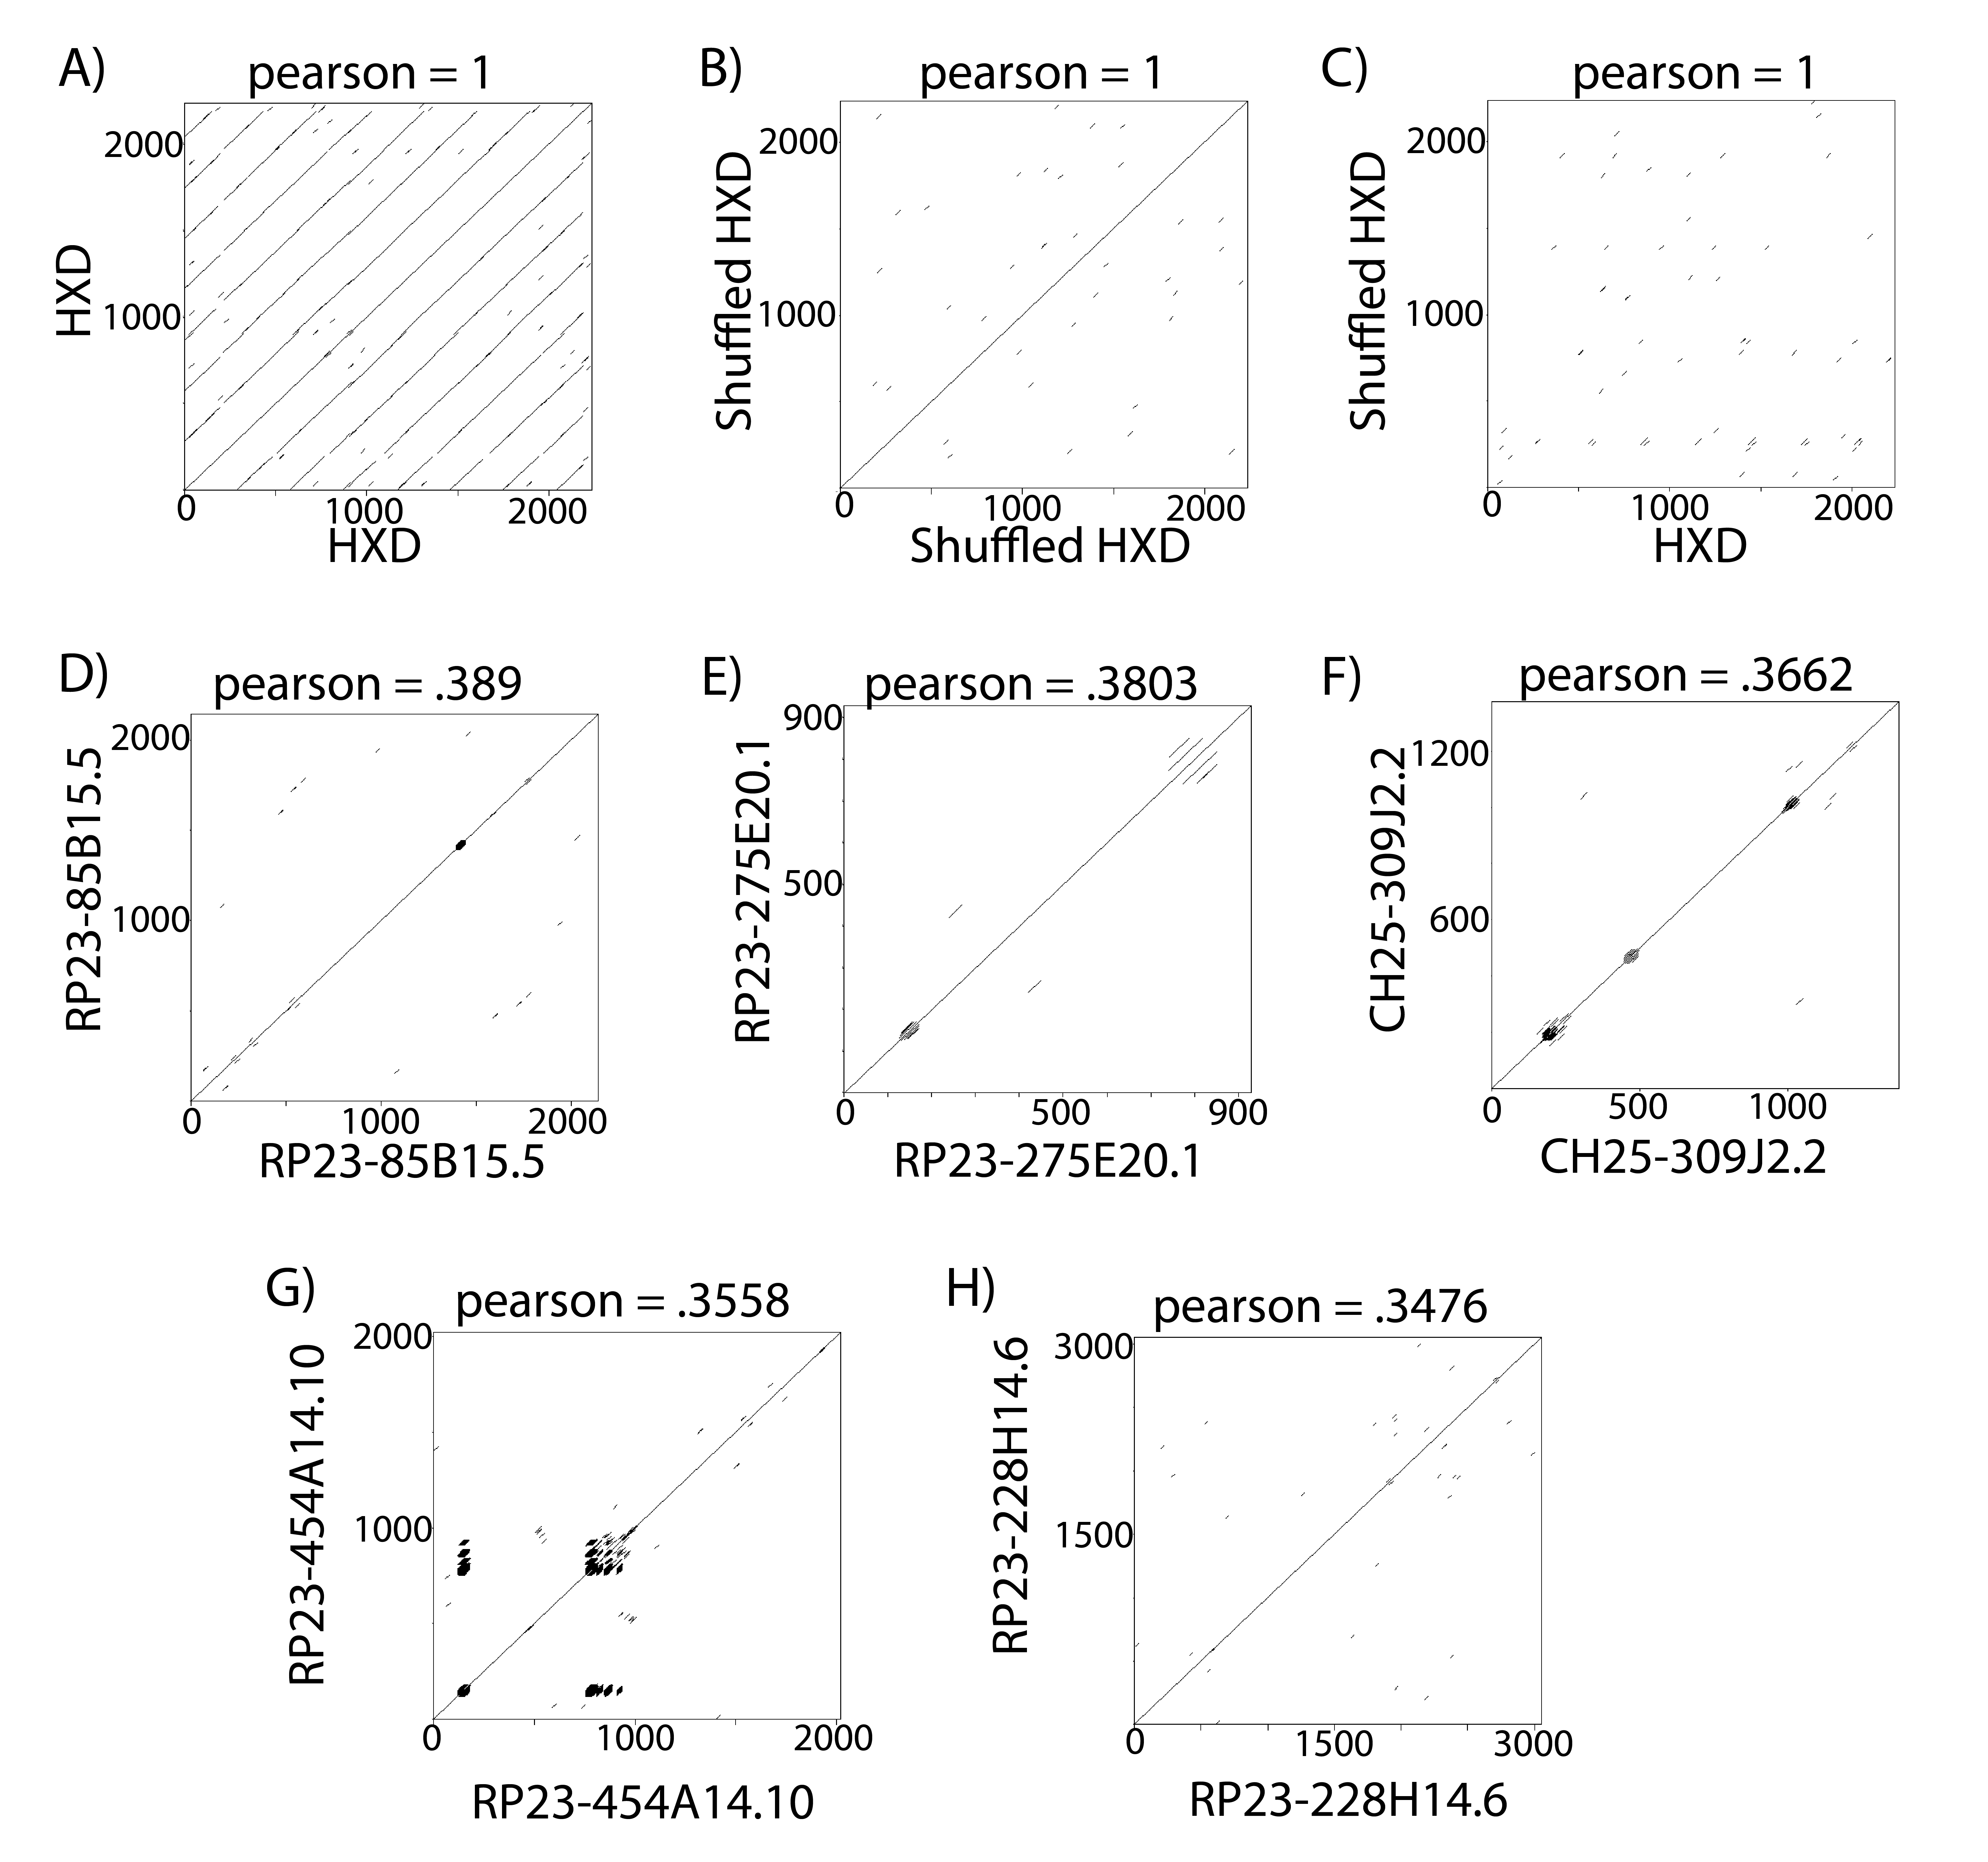
\includegraphics[width=\textwidth]{shufD.png}
\caption[Shuffling $k$-mers abrogates tandem repeat without changing motif content]{Dot plot alignments and SEEKR-defined similarity between human Xist Repeat D, shuffled Repeat D, and the top 5 mouse lncRNAs that are most similar to Repeat D. Repeat D was shuffled using $\mu$Shuffle and preserving $k$-mer content at $k$ = 4 (Jiang et al., 2008). Dotplots were generated using a window size 20 nucleotides and a threshold of 50\% identity.}
\label{fig:shufD}
\end{figure}

Therefore, a challenge in understanding lncRNA function is identifying where functional modules may be located within a sequence \cite{Pang2006RapidFunction,Hezroni2015PrinciplesSpecies,Johnson2014TheRNAs}. Clearly, the answer is not solely exonic sequence as in a protein coding reading frame. Within \emph{XIST} these sequence regions are sub-sequences within the spliced transcript \cite{Brockdorff10TheNucleus.,Brown10TheNucleus.,Brockdorff2018LocalNcRNA,Sprague2019NonlinearDomains,Pintacuda2017HnRNPKSilencing,Hoki2009AMouse,Sunwoo2017RepeatCIZ1}. Compounding the issue is that as far as is known, no specific boundary motifs (\emph{e.g.}, splice junction boundaries) are required. Potential splice junctions in genes are relatively easy to identify based off a combination of sequence content, and the presence of conserved 5' and 3' splice site motifs that demarcate the beginning and end of an intron, respectively \cite{Burge1997PredictionDNA}. 

To model this hypothesized sequence structure, we have developed an HMM that is designed to identify sub-sequences within a larger transcript that contain regions of elevated $k$-mer content to a known functional domain. Given how little is known in the field about the sequence-to-function relationship in lncRNAs, we use the archetypal lncRNA \emph{XIST} and its known functional sub-sequences (A-,B-,D-,E- repeats) as our model. 

We demonstrate here the first computational tool capable of detecting sequence similarity between functionally related but non-homologous  long non-coding RNAs in the human genome. Rather than deriving functional relationships through homology as in traditional sequence alignment \cite{Altschul1990BasicTool,Wheeler2013Nhmmer:HMMs}, we consider and model the problem of functional analogy between non-coding transcripts. lncRNAs are free to mutate at significantly faster rates than mRNAs however that lack of conservation has been shown to not necessarily imply lack of function \cite{Johnsson2014EvolutionaryFunction,Sprague2019NonlinearDomains,Nesterova2001CharacterizationSequence}. The model developed here is capable of identifying sequence features that are much too subtle and jumbled for even the most sensitive alignment algorithms to detect \cite{Wheeler2013Nhmmer:HMMs,Altschul1990BasicTool,Rice2000EMBOSS:Suite}, yet these same features have been shown to strongly predictive of function \cite{Kirk2018FunctionalContent,Sprague2019NonlinearDomains}. 

\section{Results}
\subsection{Model Structure}
Given a transcript sequence of $k$-mers, $X$, of length $L$, and a set of predefined functional features $Y$, the objective is to map each $x \in X$ to a functional state, $y \in Y$ through an HMM. Our underlying biological hypothesis is that non-coding RNAs contain sub-sequences of specific $k$-mer content that are enriched for motifs that bind a specific RBP or subset of RBPs and that these domains are free to start and stop within a larger sequence\cite{Brockdorff2018LocalNcRNA,Hezroni2015PrinciplesSpecies,Pang2006RapidFunction}. The primary purpose of the HMM is to identify the most likely positions within a sequence that these RBP-interacting functional domains begin and end. We therefore defined the first functional feature to be the \emph{query}, which is a categorical distribution of $k$-mer frequencies from training sequences known to have some specific functional role (e.g. tandem repeats of \emph{XIST}). We defined one additional functional feature which comprises a \emph{null} feature. The null state is a categorical distribution of $k$-mer frequencies that represent the average of the transcriptome, or background sequence, which is designed to encapsulate all other sequences that don't match the \emph{query}.  

The two hidden states, \textit{query} and \textit{null} are represented by the symbols ``+'' and ``-'' respectively, throughout the rest of this chapter, as this is how they are coded within the python implementation of \emph{hmmSEEKR}. 

From a probabilistic point of view, the HMM models an RNA sequence by assuming the sequence we observe ($X$) is stochastically sampled from an unknown sequence of hidden states (functional domains) that control the behavior of $X$ \cite{Rabiner1989ARecognition}. Prior HMM based models have primarily modeled the emission of a sequence of individual nucleotides and incorporated high-order interactions through conditional probabilities \cite{Burge1997PredictionDNA,Pachter2002ApplicationsProblems,Henderson1997FindingModel}. 

As an example, if the following sequence were observed, the probability of that sequence occurring could be calculated using varying amounts of prior information. Generally, the more relationships captured within the sequence, the better the sequence can be modeled (Table \ref{tbl:highorder}). 

\begin{table}[h!]
\centering
 \begin{tabular}{|c | c| c |}
 \hline
 \multicolumn{3}{|c|}{Observed Sequence $X = ATCGA$}\\
 \hline
 Markov Order & P(X) & Parameters\\
 \hline\hline
 0 & $P(A)P(T)P(C)P(G)P(A)$ & 4 \\ 
 \hline
 1 & $P(A)P(T|A)P(C|T)P(G|C)P(A|G)$ & 16\\
 \hline
 2 & $P(A)P(T|A)P(C|AT)P(G|TC)P(A|CG)$ & 64 \\
 \hline
 3 & $P(A)P(T|A)P(C|AT)P(G|ATC)P(A|TCG)$ & 256 \\
 \hline
 
\end{tabular}
\caption[Conditional dependencies in a DNA sequence]{Progressively more prior history can be incorporated to model the probability distribution of a sequence, however doing so exponentially increases the number of parameters to be estimated.}
\label{tbl:highorder}
\end{table}


Given the underlying assumptions of SEEKR \cite{Kirk2018FunctionalContent} we chose to model the emissions of $k$-mers directly rather than individual nucleotides conditioned on $k$ previous nucleotides. When constructing a parse of a sequence, this choice better represents the bag-of-words model underyling SEEKR \cite{Kirk2018FunctionalContent} while allowing each emission to be conditionally dependent only on the functional feature emitting it (Figure 3.2).

These two probabilities, \textit{e.g.} $P(ATCGA)$ \textit{vs.} $ P(A|ATCG)$, are very similar to each other, and are related by a normalizing factor. \emph{E.g.}, if $k=5$, then the probability of observing the $5$-mer $ATCGA$ is equivalent to the probability of observing $A$ given the probability of the preceding nucleotides $ATCG$, multiplied by the probability of observing $ATCG$.

$$P(ATCGA) = P(A|ATCG)P(ATCG)$$
This example illustrates another reason that we chose to model the joint probability of a $k$-mer rather than the conditional probability of a nucleotide on the preceding $k$-mer -- the joint probability distribution better models differentials between enriched and depleted $k$-mers in a bag-of-words model, whereas the conditional distribution better models longer-range interactions in the sequence. \textit{E.g.}, the $k$-mer ATCG might be quite rare in the training data, but A preceded by ATCG might have a high probability so long as it is observed, and so within the context of the HMM this sparsity of ATCG would not get modeled as desired in SEEKR.  


The last modeling choice we make is to construct the HMM such that each hidden state $y$ has a non-zero probability of transitioning to any other state, including itself. This is formally known as an ergodic HMM \cite{Rabiner1989ARecognition}. Prior HMM models of DNA sequences are primarily left-right structured \cite{Burge1997PredictionDNA,Pachter2002ApplicationsProblems,Henderson1997FindingModel,Wheeler2013Nhmmer:HMMs}, due to prior knowledge of the structure of a gene, or motif. If a model for a gene were constructed, the transition Intron $\rightarrow$ 5' UTR can be assigned a probability of zero given prior knowledge. Within lncRNAs, we and others hypothesized and shown that protein binding functional domains are modular in nature and therefore the hidden states within our HMM are free to transition in all directions.

\begin{figure}[h]
\centering
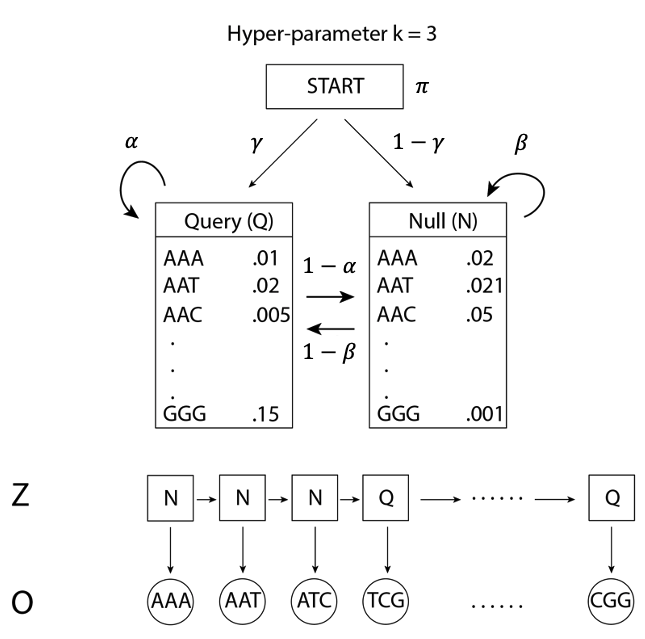
\includegraphics[width=.75\textwidth]{model.png}
\caption[Graphical model of \emph{hmmSEEKR}]{Graphical model of HMM SEEKR. The Query (``+") hidden state represents the functional domain to be identified in other lncRNA sequences and the Null (``-") hidden state represents the average $k$-mer frequencies of the transcriptome. The $\alpha$ and $\beta$ parameters represent the self-transition probabilities for the hidden state. }
\label{fig:hmmseekrmodel}
\end{figure}

\subsection{Parameter Estimation}
A hidden markov model is comprised of a stochastic transition matrix $A$, where each row vector $\psi_i$ corresponds to a categorical distribution representing the probability of hidden state $i$ transitioning to state $j$. The emission matrix $E$, where each row corresponds to a categorical distribution of $k$-mer frequencies. Finally, there is the initialization matrix $\pi$ that describes the probability of starting at each hidden state at $t=1$.
\subsubsection{Emission Parameters}
We defined the emission distribution for the query and null hidden states to be $k$-mer frequencies taken from a set of training sequences. For the query hidden state, we defined our training sets to be \emph{XIST} repeats A,B,D, and E. For the null hidden state, we defined the set of training sequences to be the set of unspliced lncRNAs in the human transcriptome. A separate HMM was trained for each \emph{XIST} repeat. 

Some of the \emph{XIST} repeats are quite short, for example \emph{XIST} repeat B is only $\approx 200$bp in length. Therefore, it is often the case that there are fewer nucleotides than there are parameters to estimate leading to zeros in the probability distribution. In reality, zero probability $k$-mers are both unlikely, as many of the motifs for RBPs that bind \emph{XIST} have no non-zero probabilities, and also mathematically intractable, as log-space for probability calculations is required for long sequences.

To correct for this parameterization problem we employed pseudo-counts, specifically we use a $+1$ pseudo-count for all $k$-mers in the training set (\emph{i.e.} initialize the counts array to 1). The hypothesis driving the pseudo-count is that despite the limited training data implying zero probability events, this only occurs because there is insufficient data to sample enough $k$-mers and their frequencies. Given the transition matrix $A$, each row $i$ (representing a hidden state's emission distribution) within $A$ is a categorical distribution $\psi_i $ comprised of the frequencies for each possible $k$-mer. It can be shown that the \emph{maximum a posteriori}, or MAP, estimate for the $k$-mer frequency distribution $\psi_i$ is achieved by adding a pseudo-count of $1$ to each $k$-mer \cite{Rabiner1989ARecognition}. This is achieved by placing a Dirichlet prior on the $k$-mer frequency distribution:

\begin{center}
    $\psi_i \sim Dir(\alpha_i^{AAA}+1,\alpha_i^{AAT}+1,\dots,\alpha_i^{GGG}+1)$
    
    $x_i \sim Cat(\psi_i^{AAA},\psi_i^{AAT},\dots,\psi_i^{GGG})$
\end{center}

The $\alpha$ parameters in the Dirichlet distribution would be the observed counts of each $k$-mer, and the +1 represents the pseudo-count. As the $\alpha$ for a given $k$-mer increases, the probability ``concentration" around that $k$-mer increases -- so when a sample of $\psi_i$ is drawn -- the $k$-mers with high $\alpha$ parameters are going to have the highest frequencies, and therefore most likely to be drawn when an observation $x_i$ is drawn. That is to say, the best estimate of the $k$-mer frequencies, given the data available and the uncertainty in it, is achieved by adding a count of $1$ to all $k$-mers. Intuitively this makes sense, as this addition has the largest impact when there is very little data to work with (less than $4^k$ $k$-mers to train from), and very little impact when there is substantial data as is the case for the null hidden state, which is trained on many thousands of $k$-mers.

\subsubsection{Transition Parameters and $k$}

We used the SEEKR algorithm to calculate a score for how well the HMM performed at identifying query-like sequence regions based off their $k$-mer similarity to the original query.  For a given set of parameters, the Kullback-Leibler diveregence was calculated between a SEEKR correlation distributions of parsed and unparsed sequences.

The KL-Divergence is defined as \cite{Brookes1951FoundationsProbability}:
\begin{equation}
    D_{KL}(P||Q) = \sum_{x\in X}P(x)\log{\frac{P(x)}{Q(x}}
\end{equation}
Where $D_{KL}$ is the KL-Divergence between two probability distributions P and Q. P represents the SEEKR score distribution of the HMM parse ``hits" (contiguously ``+'' labeled $k$-mers within the sequence) to the query sequence, and Q represent the SEEKR score distribution of unparsed sequences to the query sequence, representing a ‘reference’. If P = Q then D_{KL} = 0. D increases as the probability distributions become more dissimilar to each other. $D_{KL}(P||Q) \neq D_{KL}(Q||P)$, so for consistency $D_{KL}(P||Q)$ was always calculated. Being comprised of unparsed sequences, $Q(x)$ just depends on $k$.
In the real dataset, $P$ and $Q$ are histograms calculated from the data, and so the calculation of $D_{KL}$ compares the frequencies of SEEKR correlations in each bin for the two distributions. The larger the difference between $P$ and $Q$, the more successful the HMM was at parsing out highly correlated regions to the query.

Our goal is to find a set of parameters, $\alpha$ ($+\rightarrow +$), $\beta$ ($-\rightarrow -$), and $k$, that maximize the above expression. 
\begin{equation}
    \argmax_{\alpha,\beta,k}\sum_{x\in X}P(x|\alpha,\beta,k)\log{\frac{P(x|\alpha,\beta,k)}{Q(x|k)}}
\end{equation}


\begin{table}[h]
\centering
\begin{center}
 \begin{tabular}{|c | c| c | c |} 
 \hline
 Query & $k$ & $\alpha$ & $\beta$ \\
 \hline\hline
 Repeat A & 4 & .9999 & .9999 \\ 
 \hline
 Repeat B & 4 & .9999 & .9999\\
 \hline
 Repeat D & 2 & .75 & .9999\\
 \hline
 Repeat E & 4 & .5 & .9999\\
 \hline
\end{tabular}
\end{center}
\caption[KL-Divergence best fit parameters]{Best values of $k$, the $+\rightarrow +$ parameter $\alpha$, and $-\rightarrow -$ parameter $\beta$ as determined through a grid search based approach to identify sequences with the highest SEEKR correlation to the query.}
\label{tbl:transparams}
\end{table}

We found that $\beta$ must always be close to 1, whereas significant variance was found for the value of $\alpha$ amongst the different \emph{XIST} queries (Table \ref{tbl:transparams}). We also found that there was often significant overlap of hits between the varying sets of parameters for each query, implying that there was significant consistant regardless of general parameterization.

\subsection{Viterbi Parsing and Scoring}
The primary use for the HMM in \emph{hmmSEEKR} is identifying the most likely parse, $\phi_{max}$ for a given sequence or set of sequences, $X_i \in \{X_1,X_2,\dots,X_n\}$, where each $X_i$ is a sequence of $k$-mers. The regions that we define as ``hits" are all sub-sequences of contiguously query-labeled sequence, \emph{e.g.} for a sequence/parse pair such as:

$$(X_i=ATCGCCCG,\phi_{max}=-,-,+,+,+,+,+,+)$$

The ``hit" in this example as defined in \emph{hmmSEEKR} is the sub-sequence CGCCCG. There may be any number of hits within a sequence, but a hit is always composed of contiguous ``$+$" (query) labeled nucleotides.  The Viterbi path through each sequence was calculated as in algorithms \ref{alg:viterbi}, \ref{alg:backtrack} (Methods), and was implemented in corefunctions.py within the \emph{hmmSEEKR} package. This code can be called as in section 3.4.3 within the mSEEKR.py program.

Table \ref{tbl:hmmresults} illustrates the output of mSEEKR.py when scanning mouse \emph{Xist} using a human \emph{XIST} query. Here, an HMM was trained on human \emph{XIST} repeat A as the query hidden state, and the null hidden state was trained on the set of all unspliced lncRNAs in  mice (Methods 3.4.3,\cite{Derrien2012TheExpression}), and mouse \emph{Xist} was scanned for matches to the repeat A query. In mouse \emph{Xist}, repeat A is defined as spanning basepairs 292-713 \cite{Brockdorff10TheNucleus.}, and \emph{hmmSEEKR} called basepairs 201-748 as a hit to the repeat A query within mouse Xist (Table \ref{tbl:hmmresults}), yielding 100\% recovery of the original sequence. The score, kmerLLR as in table \ref{tbl:hmmresults}, is calculated as in Algorithm \ref{alg:LLR} and is the log-likelihood ratio of the hit. As the original definition for repeat A was formally defined by the presence of the tandem repeat \cite{Brockdorff10TheNucleus.,Brown10TheNucleus.}, and not based on functionality, such as RBP motif enrichment or experimentally determined presence of protein binding, it is significantly more challenging to accurately assess the false positive rate of the HMM (Figure \ref{fig:hnkhumanmouse}).


\begin{table}[h]
\centering
\begin{tabular}{|l|l|l|l|l|l|}
\hline 
Rank&Start & End   & Length & kmerLLR & seqName                               \\
\hline 
0     & 201   & 748    & 547     & 285.225  & \textgreater{}xist \\
1     & 10295 & 11052  & 757     & 42.734   & \textgreater{}xist \\
2     & 1532  & 1576   & 44      & 30.685  & \textgreater{}xist \\
3     & 11326 & 11450  & 124     & 29.306   & \textgreater{}xist \\
4     & 17941 & 17946  & 5       & -0.968 & \textgreater{}xist\\
\hline 
\end{tabular}
\caption[\emph{mSEEKR.py} output file]{Output of \emph{mSEEKR.py}. Each hit from scanning \emph{XIST} with an HMM trained on the A-repeat of mouse \emph{Xist} is shown and sorted by the \emph{hmmSEEKR} score, ``kmerLLR". }
\label{tbl:hmmresults}
\end{table}

\begin{figure}[h!]
\centering
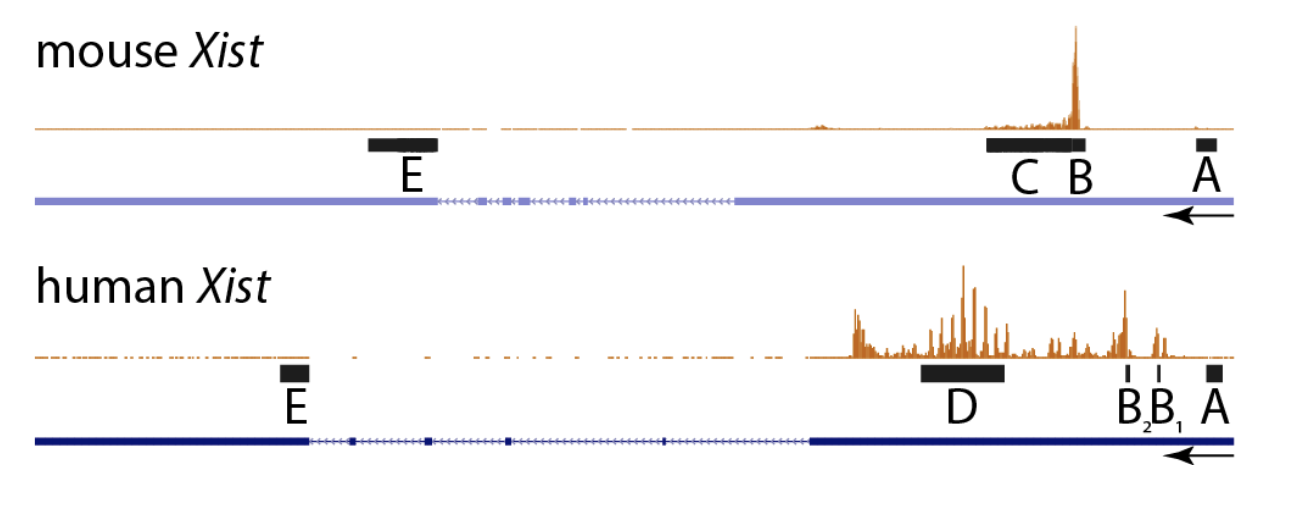
\includegraphics[width=\textwidth]{images/hnkmousehuman.png}
\caption[HNRNPK enrichment relative tandem repeat locations in human \emph{XIST} and mouse \emph{Xist}.]{UCSC wiggle- density display of HNRNPK CLIP data (orange) aligned over the mouse (mm9) and human (hg38) Xist genomic loci. Mouse and human clip data are from \cite{Cirillo2016QuantitativeEditor,VanNostrand2016RobusteCLIP}. Arrows denote direction of Xist transcription. Black rectangles indicate genomic locations of mouse and human repeat sequences used in this work.}
\label{fig:hnkhumanmouse}
\end{figure}

As there are no pre-existing annotations for these $k$-mer based sequence features within lncRNAs, it is difficult to define what constitutes a true positive and a true negative (Figure \ref{fig:hnkhumanmouse}). To help elucidate what sequence features within \emph{XIST} and other lncRNAs are functional, we turned to protein binding data for proteins that are known to bind \emph{XIST} and have been shown to be crucial for its function.

\subsection{Xist Associated RBPs}
A crucial feature of the \emph{XIST} transcript are the 4 core repeats that bind unique subsets of RNA binding proteins \cite{Sunwoo2017RepeatCIZ1,Zhao2008PolycombChromosome,Pintacuda2017HnRNPKSilencing,Wang2017TargetingGuanines,Hoki2009AMouse}. Several RBPs have been shown to be crucial for the function of \emph{XIST}, including HNRNPK, RBM15, and several others \cite{Sunwoo2017RepeatCIZ1,Zhao2008PolycombChromosome,Pintacuda2017HnRNPKSilencing,Wang2017TargetingGuanines,Hoki2009AMouse,Chu2015SystematicProteins}. The tandem repeats have been defined based only on their repetitiveness, but Figure \ref{fig:shufD} demonstrates that a non-repetitive sequence can have the same motif content as a repetitive one. Indeed, examination of ENCODE eCLIP data for HNRNPK reveals significant eCLIP binding adjacent to and extending beyond the formally defined B- and D-repeats of \emph{XIST} (Figure \ref{fig:hnkhumanmouse}). Therefore, we hypothesized that the functional elements of a lncRNA such as \emph{XIST} are not defined by repetitiveness but rather by enrichment of protein binding motifs \cite{Kirk2018FunctionalContent,Sprague2019NonlinearDomains,Dominguez2018SequenceProteins,Ray2013ARegulation,Wang2017TargetingGuanines}. To further test \emph{hmmSEEKR}, we sought to identify the proteins most associated with the A,B,D,E-repeats of \emph{XIST} so that we could validate the predictive power of our model against existing protein binding data.
\begin{figure}[h!]
\centering
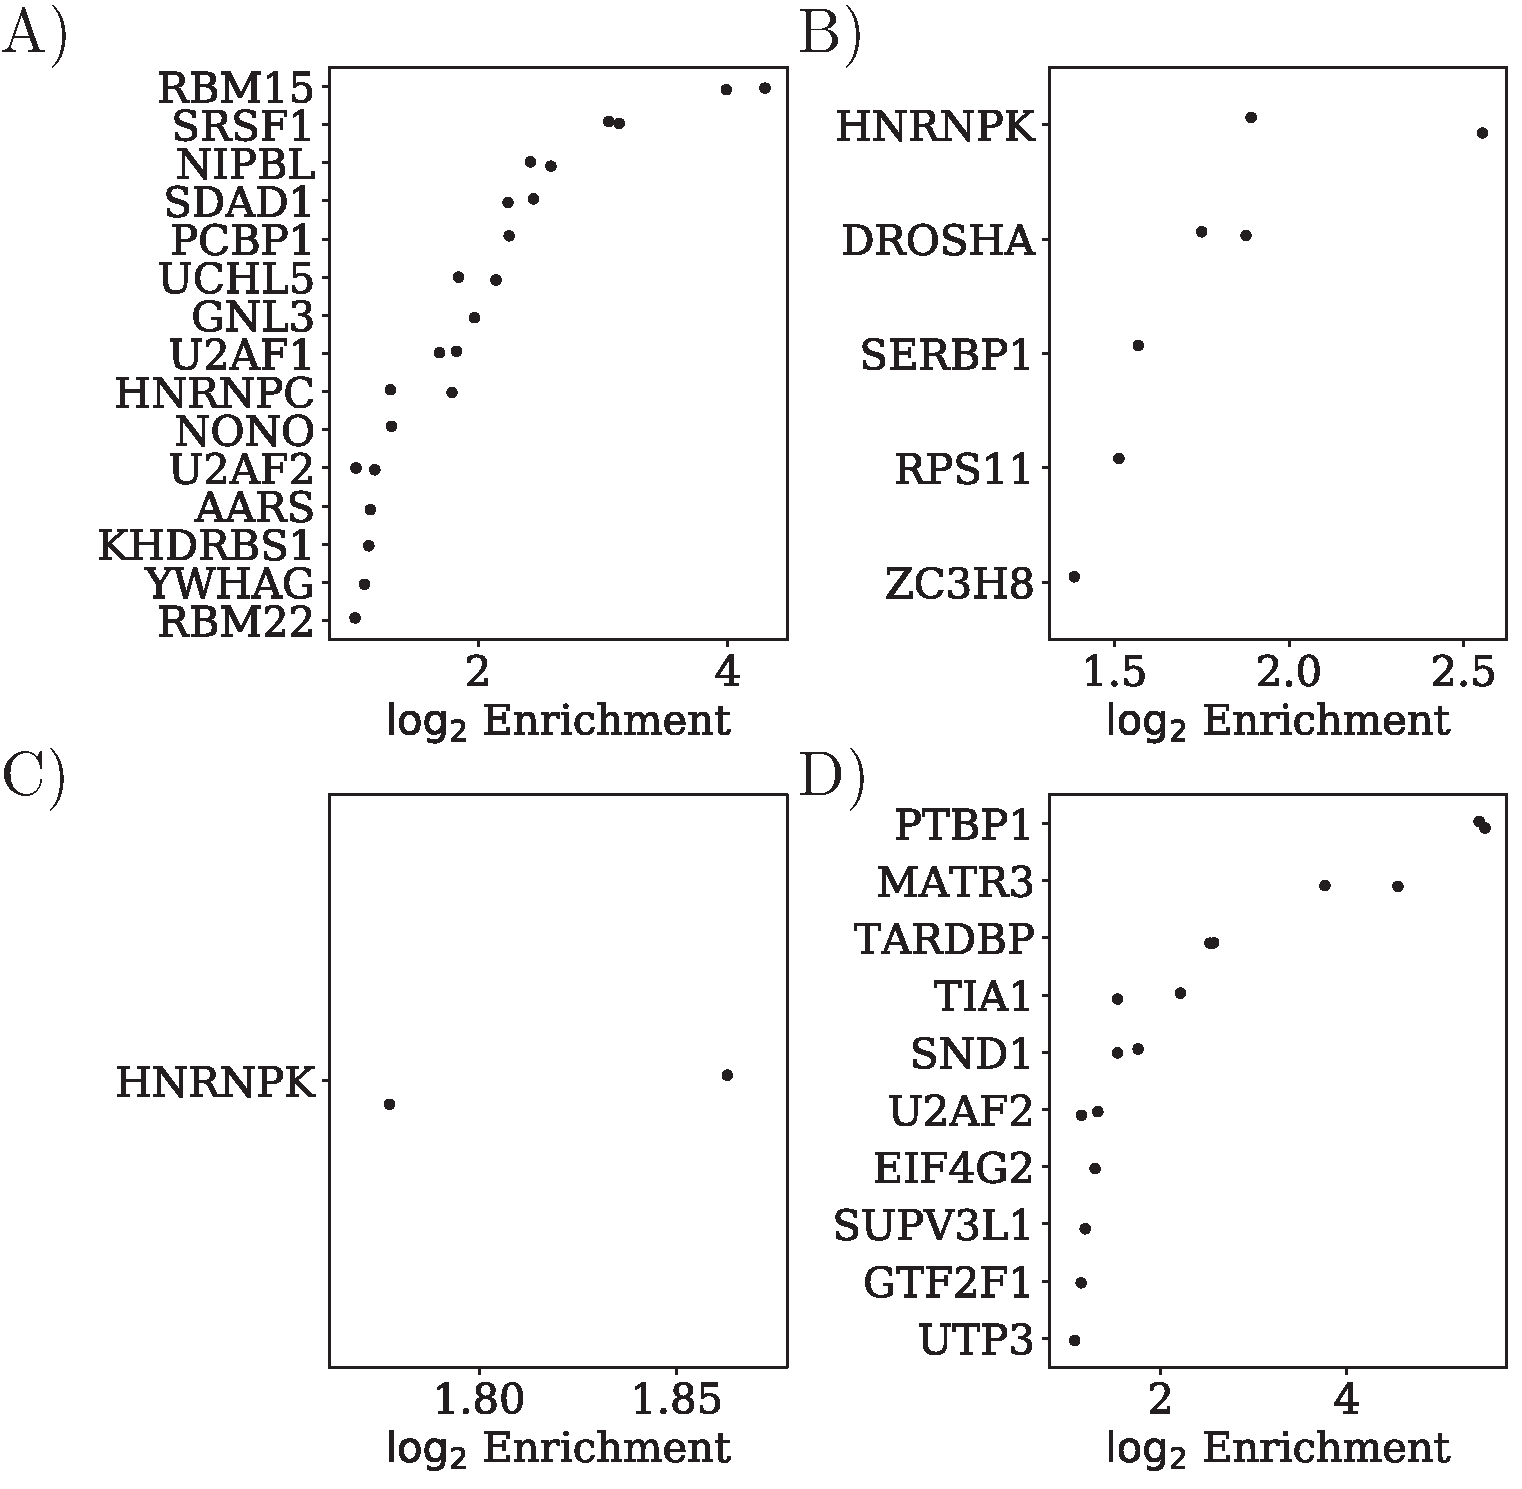
\includegraphics[width=.8\textwidth]{images/sigproteins.pdf}
\caption[\emph{XIST} tandem repeat enriched proteins]{Proteins selectively enriched within tandem repeats of \emph{XIST}. A) $\log_2$ ratio of read density for Repeat A compared to the remainder of \emph{XIST}. B) $\log_2$ ratio of read density for Repeat B compared to the remainder of \emph{XIST} is shown. C) $\log_2$ ratio of read density for Repeat D compared to the remainder of \emph{XIST}. D) $\log_2$ ratio of read density for Repeat E compared to the remainder of \emph{XIST}. A-D) Individual points within each protein represent biological replicates. }
\label{fig:xistproteins}
\end{figure}

To do this, we compared eCLIP signal for all proteins with data in the ENCODE database inside each tandem repeat relative to the remainder of the \emph{XIST} transcript. We found that each repeat within \emph{XIST} contained at least one protein that was at least 2x more enriched in within the repeat than the remainder of the \emph{XIST} transcript (Figure \ref{fig:xistproteins}A). RBM15 and SRSF1 were found to be the most specific proteins to repeat A. RBM15 is required for full \emph{XIST} silencing functionality \cite{Moindrot2015ASilencing}, and that RBM15 recruits the m6A complex to the 5' region of \emph{XIST} \cite{Patil2016M6Repression}. SRSF1 has previously been shown to bind the A-repeat of \emph{XIST} but its function within the sequence is currently unknown.


Both the B-repeat and D-repeat were found to be significantly enriched for HNRNPK over the rest of the transcript (Figure \ref{fig:xistproteins}B-C). HNRNPK is required for recruitment of PRC1 to the \emph{XIST} transcripts \cite{Pintacuda2017HnRNPKSilencing}. Deletion of the B-repeat region has previously been shown to be sufficient to abrogate \emph{XIST} dependent PRC recruitment, as well as \emph{XIST} mediated silencing. Our analysis showed that DROSHA is also enriched within the B-repeat of \emph{XIST}, however no previous studies have identified DROSHA as a direct interactor with \emph{XIST} and so the function of this interaction is unknown.

\begin{table}[h]
\centering
\begin{tabular}{|l|l|}
\hline 
\emph{Xist} Repeat&eCLIP Data                      \\
\hline 
    A&RBM15,SRSF1    \\
      B & HNRNPK\\
      D  & HNRNPK\\
      E & TIA1,MATR3,PTBP1\\
\hline 
\end{tabular}
\caption{Most enriched RBPs for each tandem repeat domain in \emph{XIST}. }
\label{tbl:eclipscan}
\end{table}

The E-repeat of \emph{XIST} was highly enriched for several proteins. The E-repeat itself is composed primarily of T-rich sequence, and therefore the proteins we observe often contain similar motifs (\cite{Ray2013ARegulation}). PTBP1, MATR3, TARDBP, and TIA1 were all found to be the most enriched within the E-repeat. PTBP1 has previously been shown to be required for proper \emph{XIST} expression and splicing during development \cite{Stork2019DevelopmentalSplicing}. TARDBP depletion is also associated with increased expression of mis-spliced \emph{XIST} transcripts \cite{Stork2019DevelopmentalSplicing}. A recent study found that MATR3 and PTBP1 form a condensate mediated by the \emph{XIST} E-repeat and this condensate is required for \emph{XIST} localization to the Xi \cite{Pandya-Jones2020AnSilencing}. 

\subsection{Detection of Rsx Domains}
Our \emph{Rsx} study in Chapter 2 relied on the existence of tandem repeats within the \emph{Rsx} transcript to perform the domain based SEEKR analysis. On a whole transcript level, \emph{XIST} and \emph{Rsx} were slightly anti-correlated despite their shared function. The relationship between the two sequences didn't become apparent until we parsed out the tandem repeats within \emph{Rsx} and performed pairwise comparisons between each \emph{XIST} tandem repeat. 

We hypothesized that we could use \emph{hmmSEEKR} to identify regions of non-linear sequence similarity between \emph{XIST} and \emph{Rsx} without \emph{a priori} identification of tandem repeats. To do this, we trained 4 separate HMMs on the A,B,D, and E-repeats of \emph{XIST} at $k\in\{2,3,4,5,6\}$ and all pairwise combinations of $\alpha,\beta \in \{.5,.75,.9,.99,.999,.9999\}$. The results outlined in Figure \ref{fig:koalarsxhmm} and Table \ref{tbl:rsxresults} are using the set of parameters that yielded the best F1 score (Methods 3.4.X). 


\begin{figure}[h!]
\centering
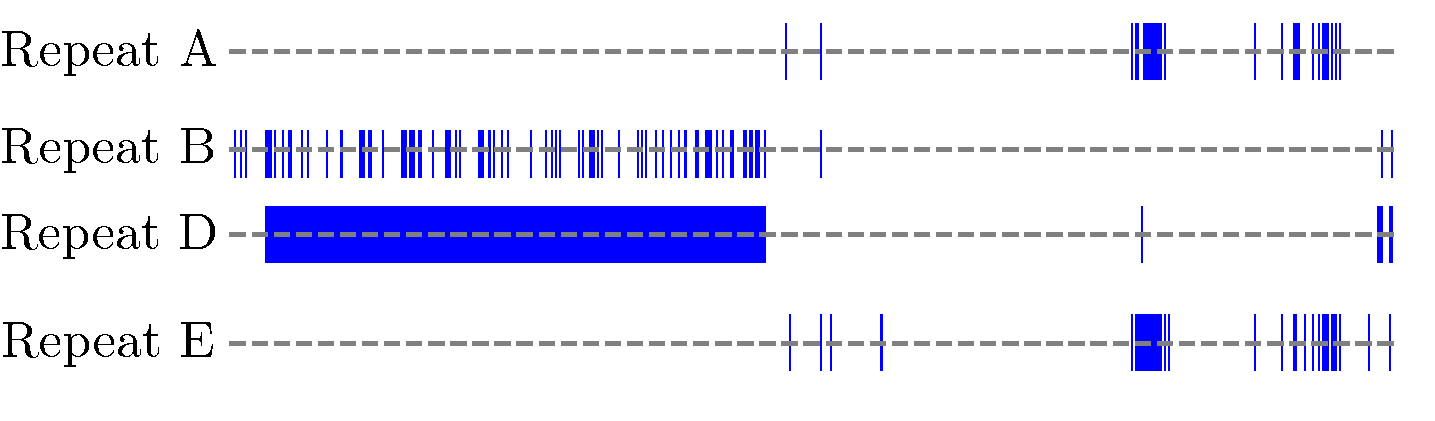
\includegraphics[width=\textwidth]{images/koalarsx.pdf}
\caption[HMM analysis of \emph{Rsx}]{\emph{hmmSEEKR} hits within koala\emph{Rsx} for an HMM trained on each \emph{XIST} repeat. Blue regions represent hits to the query, whereas dashed grey lines represent null sequence.}
\label{fig:koalarsxhmm}
\end{figure}

We found that the HMM trained on the \emph{XIST} D-repeat captured the entire tandem repeat from transcript coordinates 1,000-14,000 (Figure \ref{fig:koalarsxhmm}, Table \ref{tbl:rsxresults}). Likewise, the HMM trained on the \emph{XIST} B-repeat captured a significant portion of \emph{Rsx} repeat 1, and these regions were significantly more C-rich than the remainder of \emph{Rsx} repeat 1. Additional C-rich sequence were also identified at the 5' and 3' regions of \emph{Rsx} (Figure \ref{fig:koalarsxhmm}). The HMMs trained on the A-repeat and E-repeat both significantly aligned with \emph{Rsx} repeat 4, with 100\% precision and 25.45\% recall of the full-length repeat 4. In our original analysis, we mapped A,E-repeats to repeats 2,3, and 4 in \emph{Rsx}, however repeats 2 and 3 had relatively marginal correlation to the A,E-repeats, whereas the A,E$\rightarrow$4 relationship was the strongest of all comparisons in the original \emph{Rsx} analysis \cite{Sprague2019NonlinearDomains}. 

\begin{table}[h!]
\centering
\begin{tabular}{|l|l|l|l|l|l|}
\hline 
\emph{Rsx} Repeat Name& Start & End   & Xist Association   & Precision& Recall                      \\
\hline 
    1&  1000   & 14000    & B,D     & 98.42\% & 100\% \\
      2&17500 & 21000  & A,E     & 100\%   & 1.32\% \\
      3&21500  & 22500   & A,E      & - & 0\%  \\
      4&23000 & 27500  & A,E     & 100\%   & 25.45\% \\
\hline 
\end{tabular}
\caption[\textit{Rsx-Xist} Precision and Recall]{Precision and recall for each HMM using the tandem repeat definitions from \cite{Sprague2019NonlinearDomains}. Precision is defined as the number of correct nucleotides relative to the number of incorrect nucleotides, whereas recall is the fraction of the total domain retrieved by the HMM.}
\label{tbl:rsxresults}
\end{table}


\subsection{Sequence based prediction of RBP binding in \textit{KCNQ1OT1}}

\begin{figure}[h!]
\centering
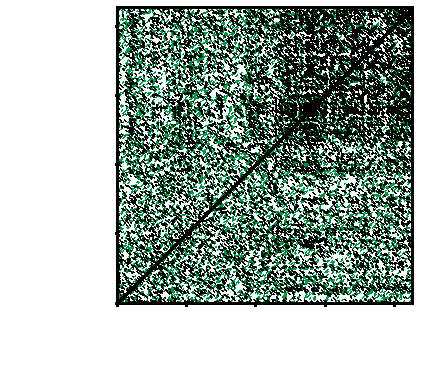
\includegraphics[width=.4\textwidth]{images/kcnd.pdf}
\caption[\emph{KCNQ1OT1} dot plot alignment]{Dot plot alignment of human \emph{KCNQ1OT1} against itself using flexidot software \cite{Seibt2018FlexiDot:Analyses}. The window parameter is 20bp and the threshold is 40\%. Black regions correspond to windows that succesfully aligned against each other. }
\label{fig:kcndot}
\end{figure}

There is at least one conserved lncRNA in the mammalian transcriptome that is known to silence gene expression in \emph{cis} through a PRC-mediated mechanism similar to \emph{XIST}, \emph{KCNQ1OT1}. The mouse \emph{Kcnq1ot1} has been shown to silence megabase scale regions of chromosome 7 and human \emph{KCNQ1OT1} silences a large region of chromosome 11. Unlike \emph{XIST}, the sequence of \emph{KCNQ1OT1} is not predominantly comprised of tandem repeat domains (Figure \ref{fig:kcndot}), barring a region in the 3' region of the sequence. Furthermore, eCLIP data for RBPs known to be essential for \emph{XIST}'s function show that they predominantly bind in the 5' half of \emph{KCNQ1OT1}'s sequence (Figure \ref{fig:kcnproteins}). Therefore, we sought to use the \emph{hmmSEEKR} package to identify functional sub-sequences within \emph{KCNQ1OT1} that are similar in $k$-mer content to \emph{XIST} A-,B-,D-, and E-repeats. 


\begin{figure}[h!]
\centering
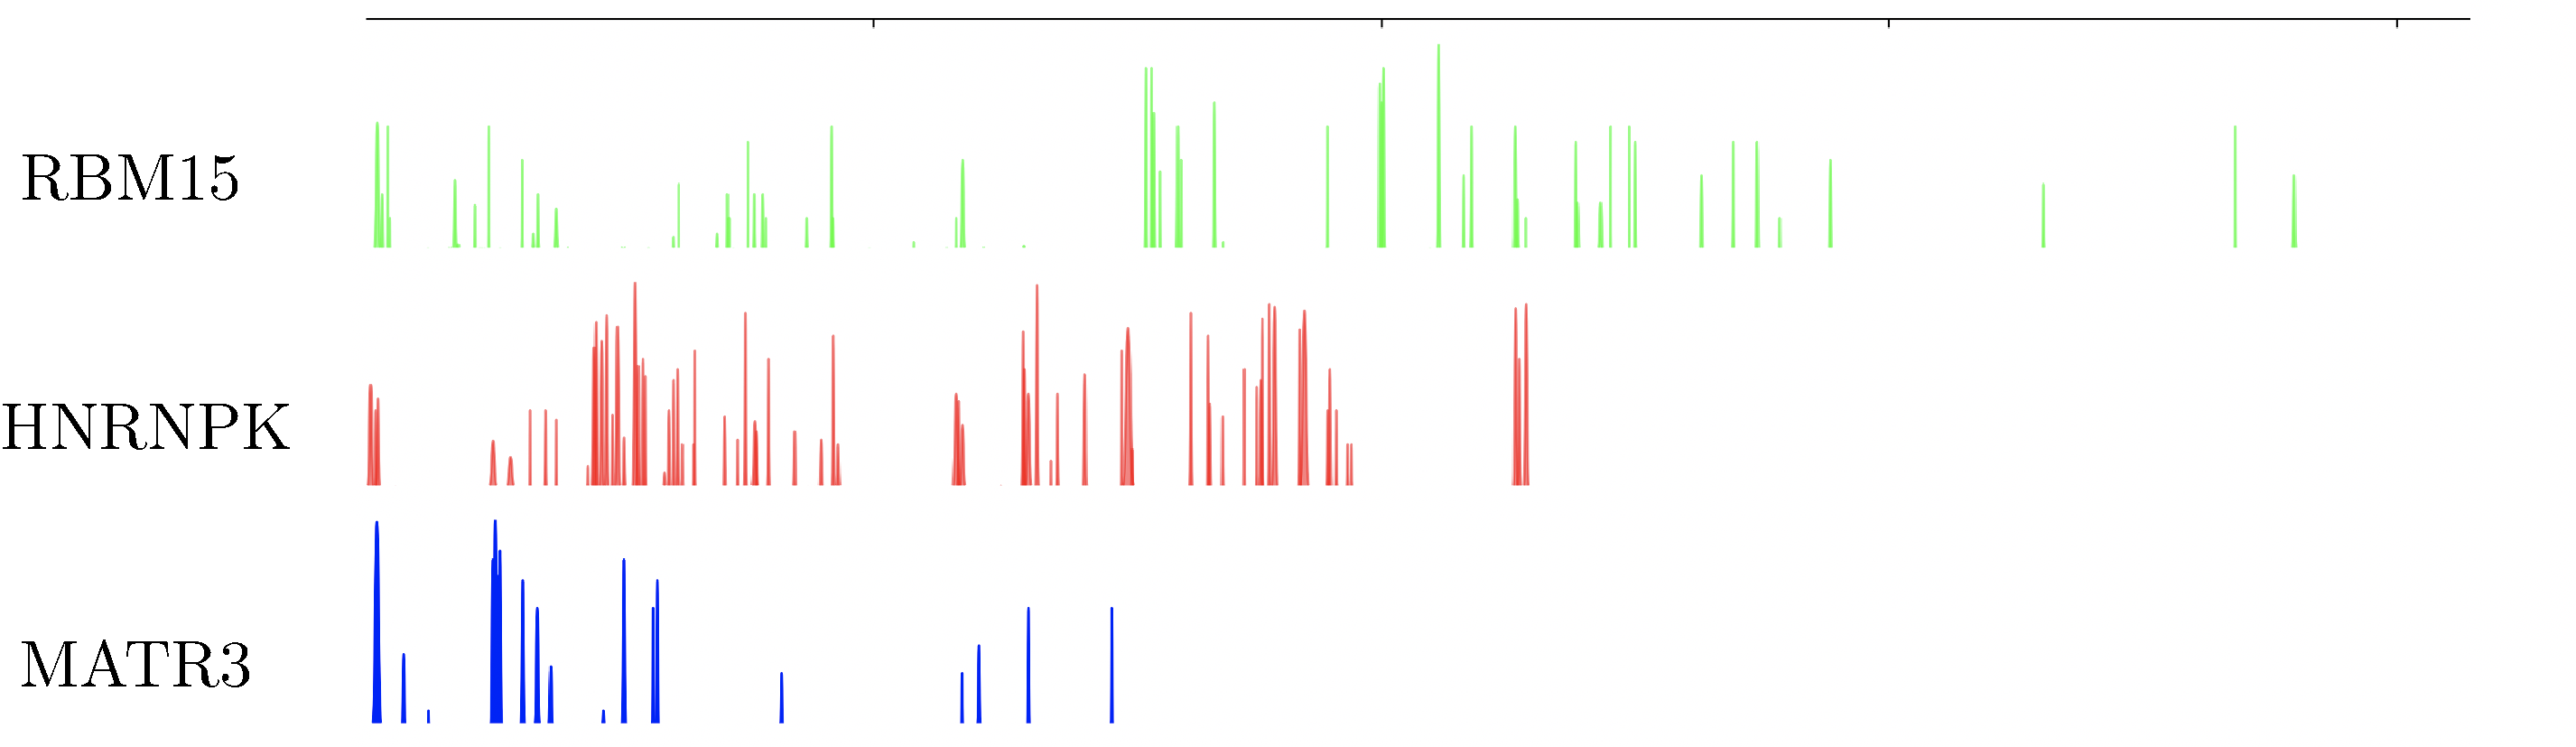
\includegraphics[width=\textwidth]{images/kcnproteins.pdf}
\caption[\emph{KCNQ1OT1} RBM15, HNRNPK, and MATR3 eCLIP tracks]{Browser tracks for RBM15 (top), HNRNPK (middle), and MATR3 (bottom) within the \emph{KCNQ1OT1} locus. Tracks represent peak intensity from ENCODE narrowPeak files for each protein, regions with no signal were not called as statistically significant peaks. }
\label{fig:kcnproteins}
\end{figure}

\emph{KCNQ1OT1} contained regions of similarity to each of the \emph{XIST} HMMs that we trained (Figure \ref{fig:kcntracks} A-D). We found that the 5' region of \emph{KCNQ1OT1}'s sequence in particular containins regions of similarity to A-,B-,D-, and E-repeats of \emph{XIST} (Figure \ref{fig:kcntracks} A-D) -- suggesting that this region of \emph{KCNQ1OT1} could be a multipurpose binder of numerous RBPs. Indeed, eCLIP data for RBM15 and SRSF1 (Figure \ref{fig:kcntracks} A), HNRNPK (Figure \ref{fig:kcntracks} B-C), and MATR3 and PTBP1 (Figure \ref{fig:kcntracks} D) reveal elevated read density for all these proteins at the 5' region of \emph{KCNQ1OT1}'s sequence. Additionally, a large portion of the inner region of \emph{KCNQ1OT1}'s sequence was identified by \emph{hmmSEEKR} to have similarity to the B- and D- repeats of \emph{Xist}. (Figure \ref{fig:kcntracks} B-C). Similar to actual B- and D-repeats of \emph{XIST}, these regions within \emph{KCNQ1OT1} correspond to elevated HNRNPK read density (Figure \ref{fig:kcntracks} B,C). 
\begin{figure}[h!]
\centering
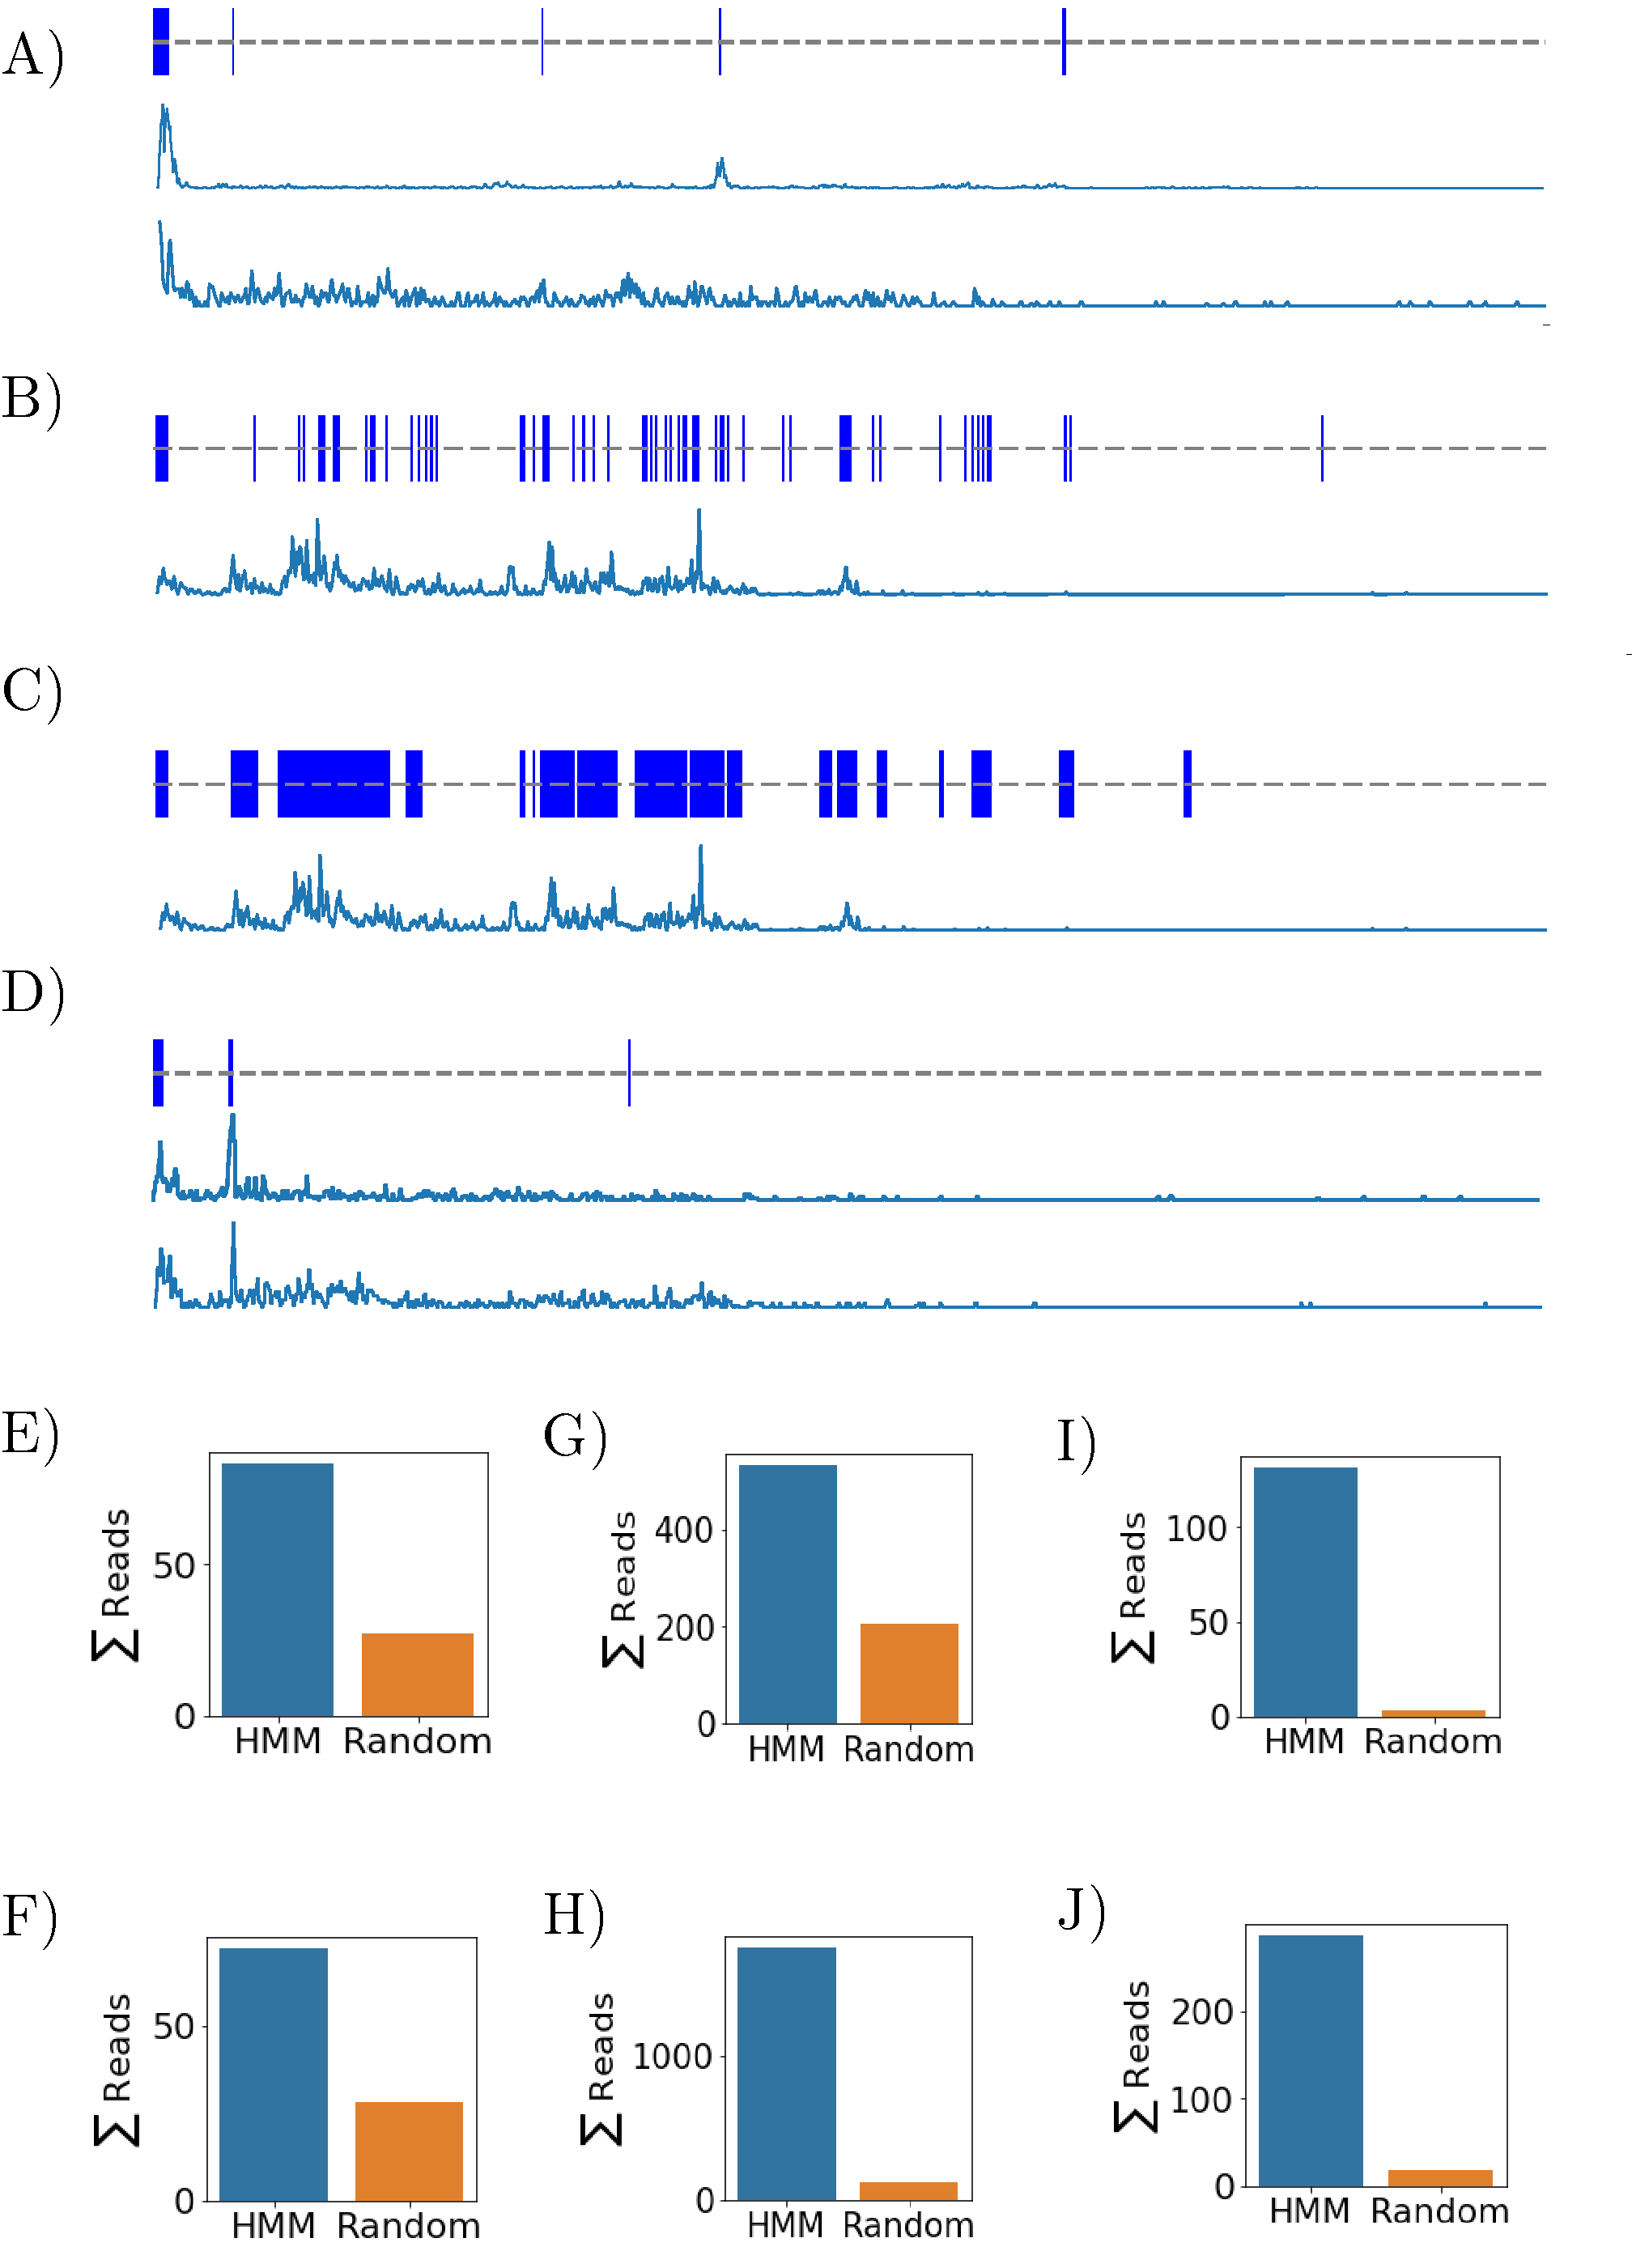
\includegraphics[width=.92\textwidth]{images/kcneclip.pdf}
\caption[Analysis of HMM and eCLIP data in \emph{KCNQ1OT1}]{\emph{hmmSEEKR} predicts \emph{XIST} associated protein binding in \emph{KCNQ1OT1}. A) HMM viterbi parse showing hits to the A-repeat in \emph{KCNQ1OT1} (blue), RBM15 eCLIP read density (middle plot), and SRSF1 eCLIP read density (bottom plot). B) HMM viterbi parse showing hits to the B-repeat (top, blue regions), and HNRNPK eCLIP read density (bottom). C) HMM viterbi parse in \emph{KCNQ1OT1} for the D-repeat (top, blue regions) and HNRNPK eCLIP read density (bottom). D) HMM viterbi parse for E-repeat in \emph{KCNQ1OT1} (top, blue regions) and eCLIP read density for MATR3 (middle) and PTBP1 (bottom). E-J) Total eCLIP reads assigned to the HMM or randomized parses for RBM15, SRSF1, HNRNPK (B-repeat), HNRNPK (D-repeat), MATR3, and PTBP1 respectively. }
\label{fig:kcntracks}
\end{figure}

We then sought to compare the read density for each protein in Table \ref{tbl:eclipscan} found within our \emph{hmmSEEKR} prediction for the associated \emph{XIST} query against a randomized shuffling of the hits found within \emph{KCNQ1OT1} (Method 3.4.6 randomization). We found that the A-repeat HMM significantly outperformed randomized shuffles for both RBM15 (Figure \ref{fig:kcntracks} E; $p< 10^{-8}$, chi-square test) and SRSF1 (Figure \ref{fig:kcntracks} F; $p< 10^{-5}$, chi-square test). HNRNPK was also significantly better predicted by the HMMs trained on the B- and D-repeats of \emph{XIST} (Figure \ref{fig:kcntracks} G,H;$p<10^{-33}$ B-repeat, $p<10^{-51}$ D-repeat, chi-square test). Finally, the E-repeat trained HMM significantly outperformed a shuffled parse for both MATR3 (Figure \ref{fig:kcntracks} I, $p<10^{-28}$,chi-square test) and PTBP1 (Figure \ref{fig:kcntracks} J; $p<10^{-43}$,chi-square test). Thus, our predictions from \textit{hmmSEEKR} would support our hypothesis that \textit{KCNQ1OT1} does contain shared sequence features with \textit{XIST}. Under the traditional hypotheses of sequence alignment, \textit{XIST} and \textit{KCNQ1OT1} have no shared sequence features \cite{Altschul1990BasicTool,Wheeler2013Nhmmer:HMMs,Rice2000EMBOSS:Suite}, however using a $k$-mer based similarity metric we have identified $>10^4$ basepairs of sequence in \textit{KCNQ1OT1} that map to functional domains in \textit{XIST}. 

\clearpage


%%%%%%%%%%%%%%%%%%%%%
%%%%%%%%%%%%%%%%%%%%%

\subsection{Transcriptome-wide RBP Prediction}
Many of the proteins that bind to \emph{XIST} and \emph{KCNQ1OT1} bind throughout the transcriptome \cite{VanNostrand2016RobusteCLIP}. Furthermore, \emph{XIST} clusters with thousands of transcripts in the human genome based on $k$-mer content \cite{Kirk2018FunctionalContent}. Therefore, we hypothesized that \emph{XIST}-like sub-sequences may be found throughout the transcriptome, both in lncRNAs as well as in pre-mRNAs. To test this hypothesis, we trained 4 HMMs on the A-,B-,D-, and E-repeats of human \emph{XIST} as in section 3.2.6 and used \emph{hmmSEEKR} to scan the set of all unspliced coding and non-coding transcripts in the human genome. The Viterbi parses for the A-,B-,D-, and E-repeat HMMs extracted sequences from the transcriptome that were significantly more similar to the query compared to the unparsed sequences (Figure \ref{fig:hmmdist}).  We then compared the results of our HMM against ENCODE eCLIP data for proteins that we have shown are enriched within each \emph{XIST} repeat (Table \ref{tbl:eclipscan}). 

\begin{figure}[h!]
\centering
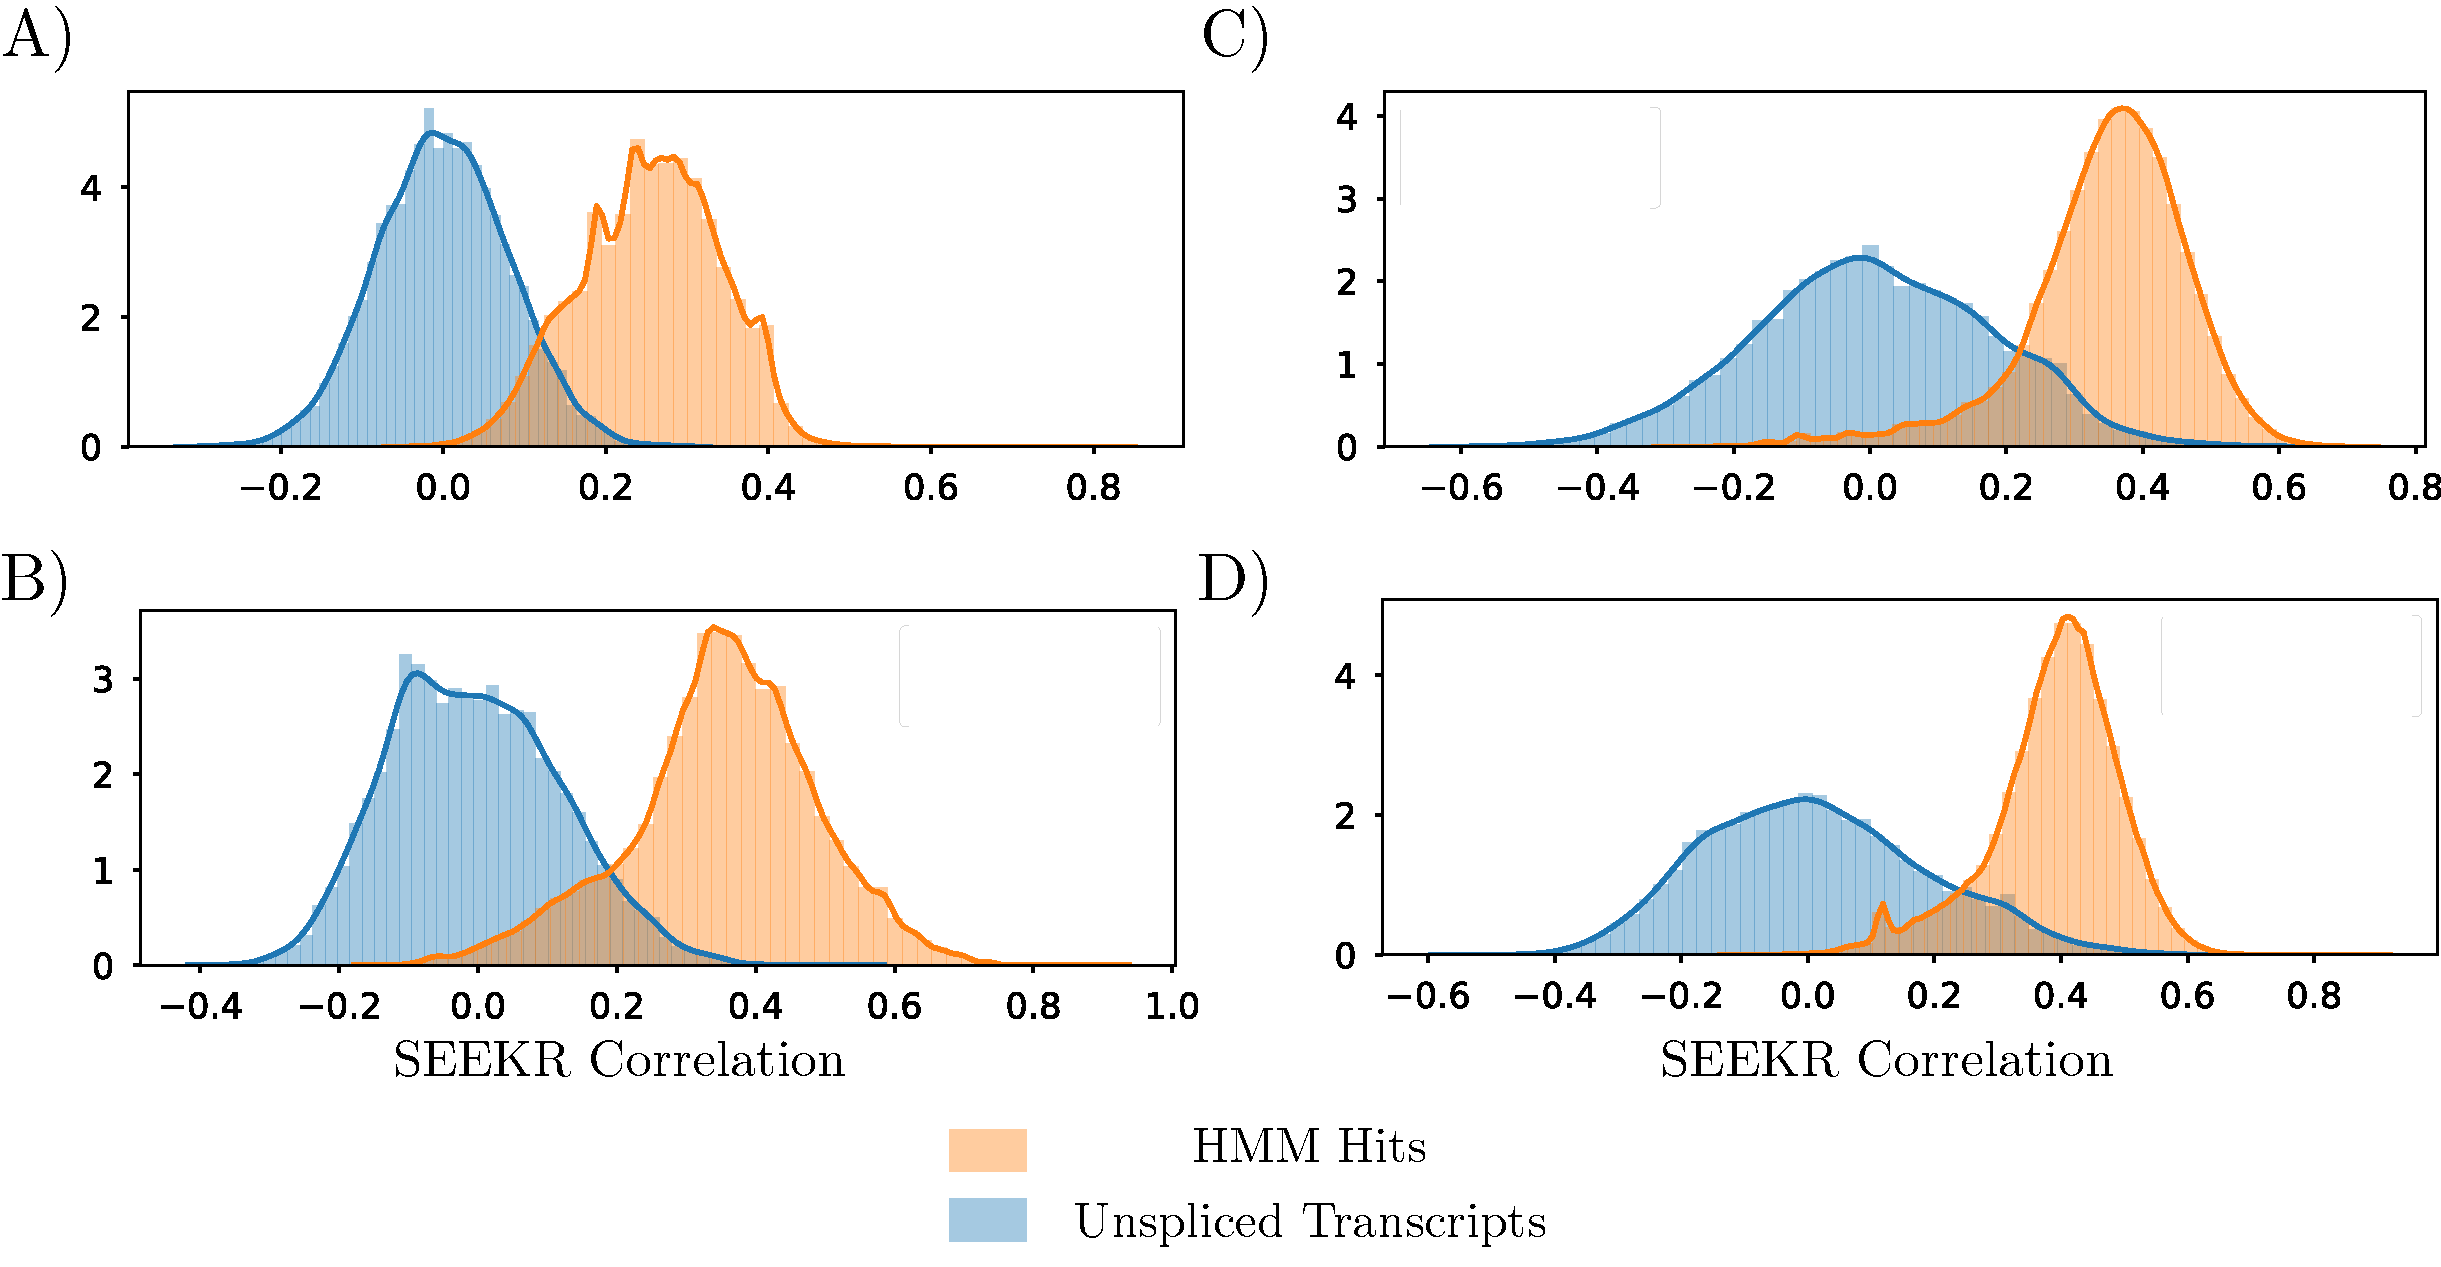
\includegraphics[width=.8\textwidth]{images/hmmdist.pdf}
\caption[\emph{hmmSEEKR} extracts sub-sequences with high correlation to query]{\emph{hmmSEEKR} models trained on \emph{XIST} tandem repeats extract sub-sequences with higher SEEKR correlation to the query than unparsed sequences using parameters listed in Table \ref{tbl:transparams}. A) A-repeat HMM hits relative to unparsed sequences, B) B-repeat HMM hits relative to unparsed sequences. C) D-repeat HMM hits relative to unparsed sequences. D) E-repeat HMM hits relative to unparsed sequences. $x$-axis represents the SEEKR correlation from the query to each transcript.}
\label{fig:hmmdist}
\end{figure}

The \emph{hmmSEEKR} HMMs significantly out-performed randomized HMM parses for each of the proteins we tested. The A-repeat trained HMM successfully captured significantly more reads for RBM15 (Figure \ref{fig:transcriptome} A left; $p\ll 10^{-100}$, chi-squared test) and SRSF1 (Figure \ref{fig:transcriptome} B left panels; $p\ll 10^{-100}$, chi-squared test) than did the randomized hits. Furthermore, true HMM hits throughout the transcriptome had significantly more reads per hit than the shuffled parses for RBM15 eCLIP data (Figure \ref{fig:transcriptome} A right panel; $p\ll10^{-100}$, student's t-test) and SRSF1 (Figure \ref{fig:transcriptome} B right panel; $p\ll10^{-100}$,student's t-test).

\begin{figure}[h!]
\centering
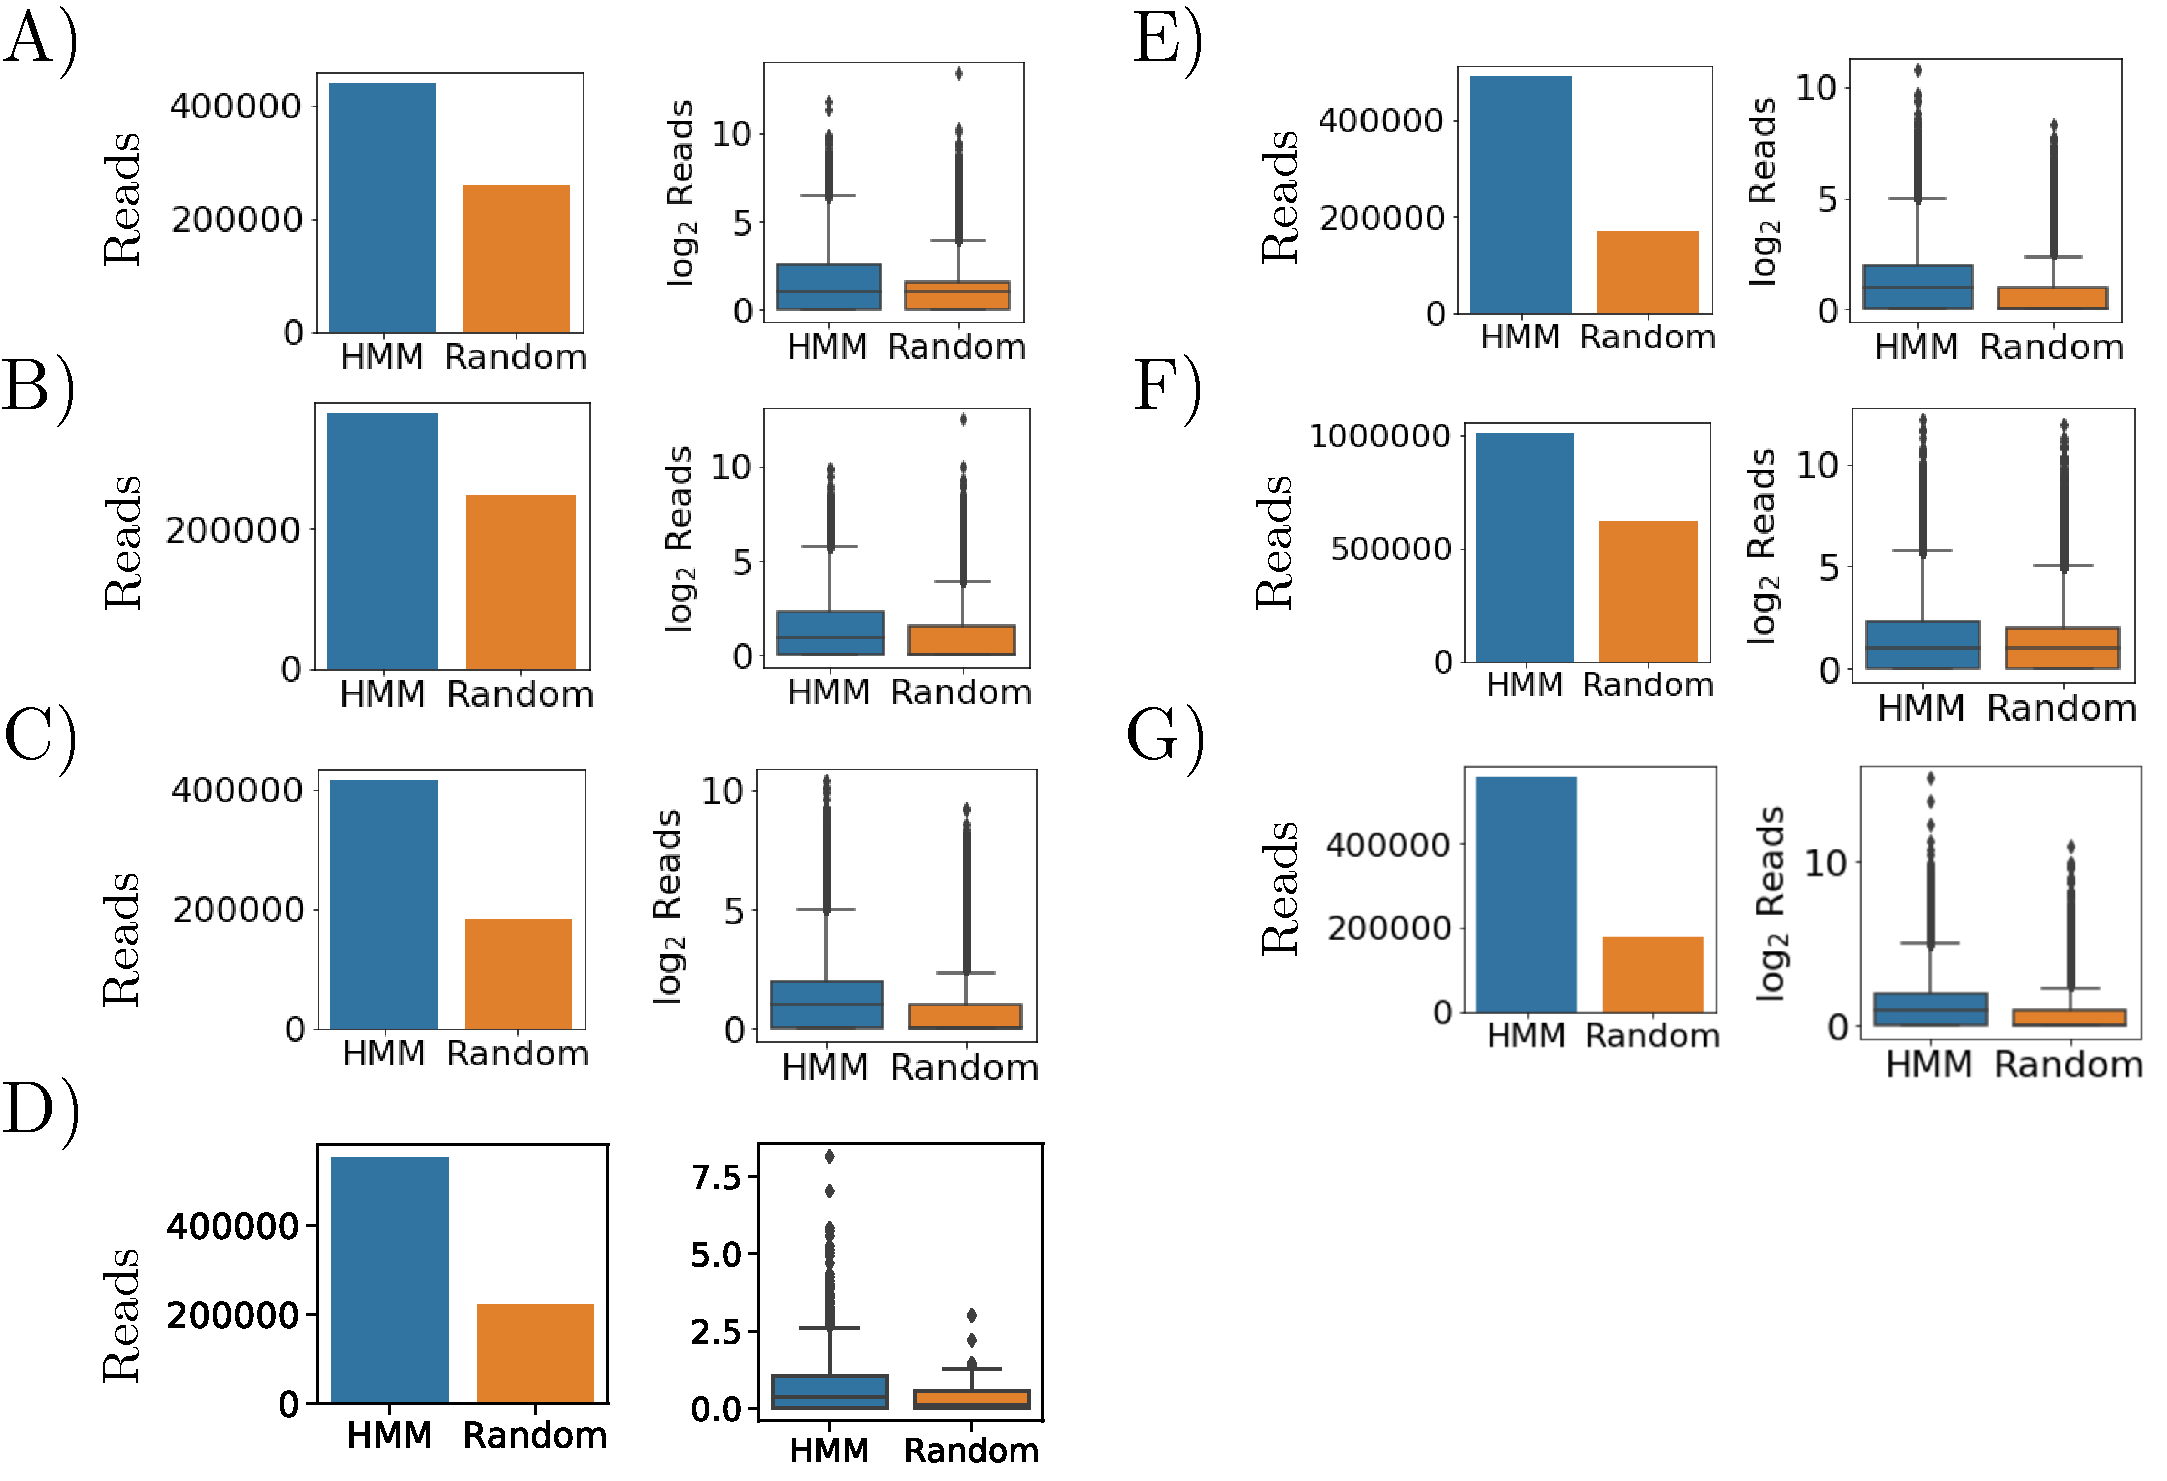
\includegraphics[width=.95\textwidth]{images/transcriptomescan.pdf}
\caption[Transcriptome-wide prediction of RBP binding regions]{\emph{hmmSEEKR} models trained on\emph{XIST} tandem repeats predict RBP binding regions throughout the transcriptome. A-G) Total number of eCLIP reads assigned to HMM Viterbi parse hits compared to randomized shuffling of hits within each transcript (left plot), and the number of reads per hit for the true HMM hits compared to the shuffled parses (right plots), for RBM15 (A), SRSF1 (B), HNRNPK B-repeat (C), HNRNPK D-repeat (D), MATR3 (E), TIA1 (F), PTBP1 (G).}
\label{fig:transcriptome}
\end{figure}

The B-repeat trained model had significantly more reads assigned from HNRNPK eCLIP data (Figure \ref{fig:transcriptome} C left-panel, $p\ll10^{-100}$, chi-squared test), and significantly more reads per hit than the randomized parses (Figure \ref{fig:transcriptome} C right-panel, $p\ll10^{-100}$,student's t-test). A similar pattern emerged with the D-repeat HMM, which captured more reads than the B-repeat HMM (Figure \ref{fig:transcriptome} C-D left-panels), and overlapped significantly more reads than randomized parses (Figure \ref{fig:transcriptome} D left-panel, $p\ll10^{-100}$,chi-square test) as well as more reads per hit than the randomized parses (Figure \ref{fig:transcriptome} D right-panel, $p\ll10^{-100}$,student's t-test). 

Finally, the E-repeat trained HMM also successfully predicted associated protein binding better than randomized parses (Figure \ref{fig:transcriptome} E-G). MATR3 had significantly more reads assigned by the true HMM (Figure \ref{fig:transcriptome} E left-panel, $p\ll 10^{-100}$,chi-square test) and more reads per hit than random (Figure \ref{fig:transcriptome} E right-panel, $p\ll 10^{-100}$, student's t-test). Intriguingly, the HMM assigned significantly more reads from TIA eCLIP (Figure \ref{fig:transcriptome} F left-panel, $p\ll 10^{-100}$, chi-squared test) but there was no significant difference in the number of reads per hit for the true HMM parses and the randomized parses (Figure \ref{fig:transcriptome} F right-panel, \emph{n.s.}, student's t-test). PTBP1 displayed the highest ratio of assigned reads between the true HMM and randomized parses over all comparisons (Figure \ref{fig:transcriptome} A-G left-panels) and assigned significantly more eCLIP reads than the randomized parses (Figure \ref{fig:transcriptome} G left-panel, $p\ll10^{-100}$, chi-squared test) as well as more reads per hit compared to random (Figure \ref{fig:transcriptome} G right-panel, $p\ll10^{-100}$, student's t-test). These data show that domains with $k$-mer based similarity to \textit{XIST} in the transcriptome are binding \textit{XIST}-associated proteins in a manner consistent with the hypotheses in \cite{Kirk2018FunctionalContent,Sprague2019NonlinearDomains}.  

%%%%%%%%%%%%%%%%%%
%%%%%%%%%%%%%%%%%%


\section{Discussion}
The non-coding portion of our genome is a vast and nebulous network of RNA transcripts whose functions are largely unknown -- and if they are, their mechanism(s) of action have proven difficult to understand. A major obstacle to better understanding lncRNA function is the relatively unknown sequence-to-function relationship in lncRNAs. In particular, even the traditional principles of conservation analysis seem to provide little insight into lncRNAs \cite{Johnsson2014EvolutionaryFunction,Pang2006RapidFunction,Nesterova2001CharacterizationSequence}. Therefore, an entirely different toolbox is needed if computational prediction of functional lncRNAs are to be made.

Our lab has recently developed a $k$-mer based algorithm for quantification of sequence similarities between non-coding transcripts \cite{Kirk2018FunctionalContent}. This method was built for comparison of full-length sequences, however it is clear from the relationship between \emph{XIST} and \emph{Rsx} that much of \emph{XIST}'s sequence bears no resemblance to \emph{Rsx} \cite{Sprague2019NonlinearDomains}, and often only small sub-sequences within a larger lncRNA may be conserved between species \cite{Pang2006RapidFunction,Nesterova2001CharacterizationSequence}. A statistical model was necessary to identify where within a sequence there are regions of non-linear sequence similarity between a sequence of interest and a query domain that has some \emph{a priori} known function.

Here, we have developed a python package, \emph{hmmSEEKR}, that uses an HMM to parse sequences of interest into regions that either have $k$-mer based similarity to some known functional domain, or not. \emph{hmmSEEKR} utilizes the underlying model of lncRNA sequence functionality in SEEKR \cite{Kirk2018FunctionalContent} as well as the hypothesis that the functionality of lncRNA can be localized within functional modules \cite{Pang2006RapidFunction, Nesterova2001CharacterizationSequence,Hezroni2015PrinciplesSpecies,Brockdorff2018LocalNcRNA,Sprague2019NonlinearDomains} in order to more precisely pin down the sequence relationship between two lncRNAs. 

We found that \emph{hmmSEEKR} was able to reproduce the non-linear sequence relationship between \emph{XIST} and \emph{Rsx} without the \emph{a priori} extraction of tandem repeat domains from \emph{Rsx} (\cite{Sprague2019NonlinearDomains}, Figure \ref{fig:koalarsxhmm}). Additionally, \emph{hmmSEEKR} identified regions of non-linear sequence similarity between \emph{XIST} and \emph{KCNQ1OT1} for each of the \emph{XIST} functional domains that an HMM was trained on. This indicates that \emph{KCNQ1OT1} contains the necessary sequence information bind the RBPs required for PRC mediated silencing, which we verified with statistical analysis of ENCODE eCLIP data \cite{VanNostrand2016RobusteCLIP}. Finally, we found that \emph{hmmSEEKR} models trained on A-,B-,D-, and E- repeats within \emph{XIST} overlapped with significantly more eCLIP reads for each models associated proteins (Table \ref{tbl:eclipscan}) than randomly generated parses, and in all cases except TIA1 the eCLIP reads per hit were significantly higher for the \emph{hmmSEEKR} parses than the randomized parses. \emph{hmmSEEKR} was therefore able to predict functional binding location for \emph{XIST}-associated proteins throughout the transcriptome. Therefore, \emph{hmmSEEKR} may be a useful tool for identification of potentially functional lncRNAs in the transcriptome. 


%%%%%%%%%%%%%%%%%%
%%%%%%%%%%%%%%%%%%


\section{Methods}
\subsection{Pseudo-code and algorithms}
The functions that drive much of analysis in the \emph{hmmSEEKR} package are found in the corefunctions.py file. These include the algorithms behind HMM analysis including the forward, backward, Viterbi, and Baum-Welch algorithm implementations. In addition, several functions crucial for parsing the supplied DNA sequences and outputting in human readable format are found within this file.

\subsubsection{$k$-mer counting}
$k$-mer counting is at the heart of both SEEKR and hmmSEEKR. This calculation is one of the simplest, but potentially most time consuming portions of the analysis. This is largely because there is no way around reading along the supplied string(s), and counting every $k$-mer as encountered. To speed $k$-mer counting up, \textbf{Algorithm \ref{alg:kmercounts}} has been implented using the cython package within Python, which is a library that allows for C-like implementation of python code.

The pseudo-code in Algorithm \ref{alg:kmercounts} is implemented in kmers.py and kmers.pyx and takes a FASTA file as input. A dictionary, or hash map, with $k$-mers as keys and their counts as values is created, and as each $k$-mer is encountered within the sequence, its value is incremented by one.

\begin{algorithm}[h]
\DontPrintSemicolon
\setstretch{1}
\SetAlgoLined
\KwResult{Python dictionary of $k$-mer counts}
 read in fasta file\;
 strFasta $\leftarrow$ concactenate fasta strings with delimiter character\;
 intL $\leftarrow$ calculate total length excluding delimiter\;
 dictKmerMap $\leftarrow$ initialize dictionary of $k$-mers with initial counts of 1\;
 \For{$k$-mer in sequence}{
  \eIf{$k$-mer in dictKmerMap }{
   dictKmerMap[$k$-mer]$\leftarrow$increment $k$-mer by 1
   }{
   do not increment\;
  }
 }
 Save binary file of python dictionary containing counts
 \caption{Counting $k$-mers from supplied sequences}
 \label{alg:kmercounts}
\end{algorithm}

\subsubsection{Ambiguous Nucleotides}
Transcripts containing regions of ambiguous sequence are of concern when building the viterbi parse, as ambiguous $k$-mers are not included in the emission distributions of the hidden state. Therefore only sequences of $k$-mers containing A,T,C, or G are allowed. To adjust for any ambiguous positions within the sequence, \textbf{Algorithm \ref{alg:ambigIdx}} stores two lists of indices. The first stores the position, or index, of each allowable $k$-mer, whereas the second stores the position of any $k$-mer containining an 'N' within it. If there are any N's within the sequence, list of $k$-mers passed into the Viterbi algorithm are split into distinct sub-sequences, because the regions flanking the ambiguous nucleotides are not adjacent to each other. Finally, when mapping the viterbi parse back to the original sequence, the two lists of indices generated above are used to merge the results back to their original order.

An example would best illustrate what this portion of the code is trying to achieve. For simplicity, let $k=1$, and our observation $X$ be: 
$$X= A,A,N,N,T,T$$
Counting indices from 1, the allowable $k$-mer indices in $X$ are:
$$\{1,2,5,6\}$$
The ambiguous $k$-mer indices are:
$$\{3,4\}$$
As the sequence $X$ is fragmented by two Ns at position 3 and 4, the flanking sequences are passed to the Viterbi algorithm to be parsed separately:
$$\{\{A,A\},\{T,T\}\}$$
Hypothetical merged results following Viterbi parse
$$\{+,+,N,N,-,-\}$$
\begin{algorithm}[h]
\DontPrintSemicolon
\setstretch{1}
\SetAlgoLined
\KwResult{Sequence of unambiguous $k$-mers}
\emph{listO}$\leftarrow$initialize empty list to contain $k$-mers\;
\emph{listIdx}$\leftarrow$initialize empty list to contain $k$-mer indices\;
\emph{listAmbigIdx}$\leftarrow$initialize empty list to contain ambig $k$-mer locations\;
\emph{listKmers}$\leftarrow$list of $k$-mers that can be constructed from ATCG\;
\emph{intIndex}$\leftarrow$0\;
 \For{k-mer \textbf{in} sequence}{
 \eIf{k-mer \textbf{in} listKmers}{
 Append \emph{$k$-mer} to \emph{listO}\;
 Append \emph{intIndex} to \emph{listIdx}\;}{
 Append \emph{intIndex} to \emph{listAmbigIdx}\;
 }
 \emph{intIndex}$+1$\;
 }
 \textbf{return} \emph{listO} \emph{listIdx} \emph{listAmbigIdx}\;
 \caption{Generate unambiguous observed sequence}
 \label{alg:ambigIdx}
\end{algorithm}

\subsubsection{Identifying hits from the Viterbi parse}
Within \emph{hmmSEEKR} a Viterbi parse is a sequence of state labels that have been assigned to each $k$-mer from a DNA sequence, \emph{e.g.} if the DNA sequence was ``AAAACCCC", and $k=4$, then the $k$-mer sequence is $\{AAAA,AAAC,AACC,ACCC,CCCC\}$, and a hypothetical Viterbi parse would be a list such as $\{-,-,-,+,+\}$, where ``$-$" represents the null state, and ``$+$" represents the query state. \textbf{Algorithm \ref{alg:groupHMM}} takes the list $\{-,-,-,+,+\}$ and converts it into a grouped list, \emph{e.g.} $\{\{-,-,-\},\{+,+\}\}$. This also exactly defines what term a hit within our HMM, consecutively labeled ``$+$" regions with a sequence from the viterbi parse.
\begin{algorithm}[h]
\DontPrintSemicolon
\setstretch{1}
\SetAlgoLined
\KwResult{Viterbi backtrack grouped into consecutive states}
\emph{condition}$\leftarrow$Swap condition, \emph{i.e.} '-' encountered\;
\emph{Key}$\leftarrow$Stores a FLAG that switches value when condition is met\;
\emph{previousNuc}$\leftarrow$Previous nucleotide\;
\For{nucleotide in sequence}{
\emph{currNucBool}$\leftarrow$TRUE/FALSE is \emph{nucleotide} in \emph{condition}\;
\emph{prevNucBool}$\leftarrow$TRUE/FALSE is \emph{previousNuc} in \emph{condition}\;
\eIf{currNucBool$\neq$prevNucBool}{swap \emph{Key}\;}{\emph{Key}\;}
\emph{previousNuc}$\leftarrow$nucleotide\;
}
 \caption{Group HMM hits}
 \label{alg:groupHMM}
\end{algorithm}

\subsubsection{HMM Score}
The score for the HMM is calculated for each ``hit" within the transcript, as defined in the prior section. We assume that the set of state labels from the Viterbi algorithm are now known. This allows, for a hit $X$ of length $L$, the likelihood that $X$ was emitted from the query state over its entire length. 

$$P(X=\{x_1,\dots,x_L\} | Y = \{+,\dots,+\}) = \prod_{i=1}^L{p(x_i|+)}$$

This likelihood can be compared to the likelihood of $X$ had it been emitted from the null state, and a likelihood ratio can be calculated.

$$S' = \frac{\prod_{i=1}^L{p(x_i|+)}}{\prod_{i=1}^Lp(x_i|-)}$$

Due to the lengths of most sequences, these calculations are moved to log-space, yielding the formula for the score reported by \emph{hmmSEEKR}. These calculations are implemented in Algorithm \ref{alg:LLR}.

$$S = \sum_{i=1}^L{\left[\log_2 p(x_i|+)- \log_2 p(x_i|-)\right]}$$
\begin{algorithm}[h]
\DontPrintSemicolon
\setstretch{1}
\SetAlgoLined
\emph{arrLLR}$\leftarrow$empty array with an element for each hit\;
\emph{hits}$\leftarrow$list of sequences that HMM called hits\;
\emph{Query}$\leftarrow$Frequency distribution of kmers in query\;
\emph{Null}$\leftarrow$Frequency distribution of kmers in null\;

\For{hit \textbf{in} hits}{
\emph{intLLRQuery}$\leftarrow$ 0\;
\emph{intLLRNull}$\leftarrow$ 0\;
\For{kmer \textbf{in} hit}{
\emph{intLLRQuery}$+\log{P(kmer|Query)}$\;
\emph{intLLRNull}$+ \log{P(kmer|Null)}$\;
}
\emph{arrLLR[hit]}$\leftarrow$\emph{intLLRQuery}-\emph{intLLRNull}\;
}
 \caption{Log-likelihood}
 \label{alg:LLR}
\end{algorithm}

\subsubsection{Viterbi Parse}

The premise behind the Viterbi algorithm is outlined in the introduction. Briefly, we seek to find the sequence of hidden states that maximizes the joint probability function of the HMM defined in equation \ref{eq:jointhmm}, given the observations $X$, the transition matrix $A$, the emission matrix $E$, and the initial probabilities of each hidden state $\pi$. The viterbi algorithm is implemented in \emph{hmmSEEKR} as in \textbf{Algorithm \ref{alg:viterbi}}.

At each step in the Viterbi algorithm, the state transition that maximizes the probability at time $t$ is recorded, for each state. That is, at time $t$, the ``+" state has a most liekly transition from either ``+'' or ``-" from time $t-1$, and the ``-" state at time $t$ has a most likely transition from either ``+" or ``-" from time $t-1$ in the sequence. To identify which was the most likely, a backtrace must be calculated after all these calculations have been made, and this is implemented in \textbf{Algorithm \ref{alg:backtrack}}.

\begin{algorithm}[H]
\DontPrintSemicolon
\setstretch{1}
\SetAlgoLined
\emph{O}$\leftarrow$Sequence of kmers\;
\emph{E}$\leftarrow$Emission matrix\;
\emph{A}$\leftarrow$Transition matrix\;
\emph{$\pi$}$\leftarrow$Starting probability of each state\;
\emph{states}$\leftarrow$ List of states \emph{i.e.} [-,+]\;
\emph{dictViterbi}$\leftarrow$List of dicts with cumulative probability at each time $t$ for each state\;
\;
\emph{dictViterbi[1][query]} means the cumulative probability at time $t=1$ at state=query\;\;
\emph{dictMaxState}$\leftarrow$List of dicts containing the state at time $t-1$ that maximized transition to each state at time $t$\;
\;
\;
Initial probabilities at each state at time $t=1$\;
\For{state \textbf{in} states}{
\emph{dictViterbi[1][state]}$\leftarrow \log{P(state|\pi)}+\log{P(O_1|state)}$
}
\;

Calculate probability of being in each state at time $t$ and find which state transition maximizes this probability\;
\For{t \textbf{in} range(2,length of O)}{\;
Add new dictionary element to dictViterbi and dictMaxState
\;
\For{state \textbf{in} states}{\;
selectedState$\leftarrow$ start with the first state to calculate prob\;
currMaxProb$\leftarrow \log P(state|selectedState)+dictViterbi[t-1][selectedState]$\;
\;
\For{checkState in remaining states}{\;
tempProb$\leftarrow \log P(state|checkState)+dictViterbi[t-1][checkState]$\;\;
\eIf{tempProb$>$currMaxProb}{set currMaxProb to tempProb\;}{keep currMaxProb the same\;selectedState$\leftarrow$checkState\;}
}
currMaxProb$\leftarrow$currMaxProb$+\log P(O_t|state)$\;
\emph{dictViterbi[t][state]}$\leftarrow$currMaxProb\;
\emph{dictMaxState[t][state]}$\leftarrow$selectedState\;
}
}
 \caption{Viterbi parse}
 \label{alg:viterbi}
\end{algorithm}

\begin{algorithm}[h]
\DontPrintSemicolon
\setstretch{1}
\SetAlgoLined

\emph{backtrack}$\leftarrow$empty list to append maximizing states to\;
\emph{dictViterbi}$\leftarrow$List of dicts with cumulative probability at each time $t$ for each state\;
\;
\emph{dictViterbi[1][query]} means the cumulative probability at time $t=1$ at state=query\;\;
\emph{dictMaxState}$\leftarrow$List of dicts containing the state at time $t-1$ that maximized transition to each state at time $t$\;
\;
\;
maxProbability$\leftarrow$largest probability at time $t=T$\;
maxState$\leftarrow$state associated with maxProbability\;
maxPriorState$\leftarrow$dictMaxState[T][maxState], get state that transitioned to maxState at $t=T-1$\;
\;
Append maxPriorState to backtrack\;

\For{t=T-2 to t=1}{
Append dictMaxState[t+1][maxPriorState] to backtrack\;
maxPriorState$\leftarrow$dictMaxState[t+1][maxPriorState]
}

\textbf{return} backtrack with order flipped to start at $t=1$

 \caption{Backtrack viterbi}
 \label{alg:backtrack}
\end{algorithm}

\clearpage

\subsubsection{Baum-Welch Algorithm}

The Baum-Welch algorithm uses the forward and backward algorithms to iteratively calculate the expected number of state transitions from a training set of sequences. Given that we do not wish to update the $k$-mer frequency distributions, the algorithm was implemented in \emph{hmmSEEKR} to only update the transition matrix $A$. 

\begin{algorithm}[H]
\DontPrintSemicolon
\setstretch{1}
\SetAlgoLined
\emph{X}$\leftarrow$Sequence of kmers\;
\emph{Y}$\leftarrow$Sequence of hidden states\;
\emph{E}$\leftarrow$Emission matrix\;
\emph{A}$\leftarrow$Transition matrix\;
\emph{$\pi$}$\leftarrow$Starting probability of each state\;
\emph{states}$\leftarrow$ List of states \emph{i.e.} [-,+]\;
\;

$\alpha(t)\leftarrow$forward probabilities\;
$\beta(t)\leftarrow$backward probabilities\;\;

$\gamma_{i}(t)\leftarrow \frac{P(Y_t=i,X|A,E,\pi)}{P(X_t)}$ ; probability of being in state i at time t\;
$\epsilon_{ij}(t)\leftarrow \frac{P(Y_t=i,Y_{t+1}=j,X|A,E,\pi)}{P(X_t)}$ ; probability of being in state i at time t and state j at time t+1\;
\;

\For{each time "t" in sequence X}{
\For{state "i" in states}{
$\log P(X_t)\leftarrow \textrm{logsumexp}\left(\alpha_i(t)+\beta_i(t)\right)$\;
$\gamma_i(t)\leftarrow \alpha_i(t)+\beta_i(t) - \log P(X_t)$\;
\For{state "j" in state}{
$A_{ij}(t+1)\leftarrow \log P(Y_{t+1}=j|Y_t=i)$\;
$E_j(t+1)\leftarrow \log P(X_{t+1}|Y_{t+1}=j)$\;
numerator$\leftarrow \alpha_i(t)+A_{ij}(t) + \beta_j(t+1)+E_j(t+1)$\;
denominator$\leftarrow \log P(X_t)$\;\;
$\epsilon_{ij}(t)\leftarrow$numerator-denominator\;
}
}
Append new entry to $\gamma$ list of dicts\;
Append new entry to $\epsilon$ list of dicts\;
}

Sum $\gamma$ and $\epsilon$ over all values of $T$ for all states $i$ and $j$. The sum below represents the expected number of transitions from state $i$ to state $j$ over the sequence. 
$$A^*_{ij} = \frac{\sum_t{\epsilon_{ij}(t)}}{\sum_t{\gamma_{i}(t)}} $$\;

Do not update emission matrix $E$.\;\;
\textbf{return} $A^*$\;

 \caption{Baum Welch Parameter Update}
 \label{bw}
\end{algorithm}

\subsubsection{Forward Algorithm}
The forward algorithm calculates the likelihood of the data, $P(X)$, as well as the probability of the sequence $x_{1:t}$ ending at state $i$ at time $t$. The algorithm was implemented through the pseudo-code below in \emph{hmmSEEKR}. 

\begin{algorithm}[H]
\DontPrintSemicolon
\setstretch{1}
\SetAlgoLined
\emph{X}$\leftarrow$Sequence of kmers\;
\emph{Y}$\leftarrow$Sequence of hidden states\;
\emph{E}$\leftarrow$Emission matrix\;
\emph{A}$\leftarrow$Transition matrix\;
\emph{$\pi$}$\leftarrow$Starting probability of each state\;
\emph{states}$\leftarrow$ List of states \emph{i.e.} [-,+]\;
\;

$\alpha_i(t)\leftarrow$forward probabilities, indexed by time $t$ and state $i$ \emph{i.e.} the probability of being in state $i$ at time $t$\;
$T\leftarrow$length of X\;\; 

Initialize probabilities at $t=1$\;
$\alpha_i(t=1)\leftarrow \pi(i) + \log P(X_t |Y_t = i)$\;\;
\For{t in T}{
Append new entry to $\alpha$\;
\For{state "i" in states}{
currP$\leftarrow$\{+:0,-:0\} : dict with entry for each state, indexed by state name\;
\For{state "j" in states}{
$A_{ij}(t)\leftarrow P(Y_t=i|Y_{t-1}=j)$\;
currP[j]$\leftarrow \alpha_j(t-1) + A_{ij}(t)$\;
}
$\alpha_i(t)\leftarrow \textrm{logsumexp}\left(currP\right)+\log P(X_t|Y_t=i)$\;
}
}
 \caption{Forward Algorithm}
 \label{fwd}
\end{algorithm}

\subsubsection{Backward Algorithm}
The backward algorithm calculates the probability of the observed sequence $P(X)$, as well as the probability of sequence $x_{t+1:T}$ starting in state $i$ at time $t$. The algorithm was implemented as below in \textit{hmmSEEKR} and is primarily used in the Baum-Welch algorithm. 

\begin{algorithm}[H]
\DontPrintSemicolon
\setstretch{1}
\SetAlgoLined
\emph{X}$\leftarrow$Sequence of kmers\;
\emph{Y}$\leftarrow$Sequence of hidden states\;
\emph{E}$\leftarrow$Emission matrix\;
\emph{A}$\leftarrow$Transition matrix\;
\emph{$\pi$}$\leftarrow$Starting probability of each state\;
\emph{states}$\leftarrow$ List of states \emph{i.e.} [-,+]\;
\;

$\beta_i(t)\leftarrow$backward probabilities, indexed by time $t$ and state $i$ \emph{i.e.} the probability of being in state $i$ at time $t$\;
$T\leftarrow$length of X\;\; 

Initialize probabilities at $t=T$\;
$\beta_i(t=T)\leftarrow 0$ ; probability of 1 in log space\;\;
\For{T to t=1}{
Append new entry to $\beta$\;
\For{state "i" in states}{
currP$\leftarrow$\{+:0,-:0\} : dict with entry for each state, indexed by state name\;
\For{state "j" in states}{
$A_{ij}(t)\leftarrow P(Y_{t+1}=j|Y_{t}=i)$\;
$E_j(t+1)\leftarrow P(X_{t+1}|Y_{t+1}=j)$\;
currP[j]$\leftarrow \beta_j(t+1) + A_{ij}(t) + E_j(t+1)$\;
}
$\beta_i(t)\leftarrow \textrm{logsumexp}\left(currP\right)$\;
}
}

\textbf{return} $\beta$ inverted s.t. $1\rightarrow T$ rather than $T \rightarrow 1$\;
 \caption{Backward Algorithm}
 \label{bwd}
\end{algorithm}

\clearpage

\subsection{Python implementation}
\begin{table}[t!]
\centering
 \begin{tabular}{|p{3cm}|p{5cm}|p{5cm}|}
 \hline
 Program & Input & Purpose\\
 \hline\hline
 kmers.py & fasta file & Count $k$-mers within fasta files provided \\ 
 \hline
 train.py & counts files from kmers.py for query and null & Generate matrices that define the HMM\\
 \hline
 mSEEKR.py & fasta file for sequence(s) of interest, path to output of train.py & retrieve the viterbi parse of the sequence of interest to identify potential functional domains \\
 \hline
bw.py & HMM training sequences, initial parameterizations & provide MLE of transition parameters \\
 \hline
 
\end{tabular}
\caption{Individual programs within the \emph{hmmSEEKR} package.}
\label{programs}
\end{table}
\emph{hmmSEEKR} has been implemented as a python package in order to rapidly train HMMs and scan sequences of interested for potential function domains. Given the general algorithms defined above, which roughly correspond to individual functions within the \emph{hmmSEEKR} package, a thorough guide is provided for how the algorithms have been implemented. 

\subsubsection{Installation}
Table \ref{programs} provides an overview of the different python programs within the \emph{hmmSEEKR} package. The first step is to ensure that Python3.6 or greater is installed, as well as the SEEKR package and hmmSEEKR repository which can be retrieved entering the following commands:

\begin{verbatim}
> pip install seekr
> git clone https://github.com/spragud2/mSEEKR
> cd mSEEKR/
> python setup.py build_ext --inplace
\end{verbatim}

\subsubsection{$k$-mer frequencies}
To count $k$-mers for a set of sequences, a single fasta file containing any number of sequences is required. The program counts the $k$-mers in all sequences, and then calculates the average over all of them to provide a single distribution of $k$-mer frequencies. Additionally the program is capable of multi-processing over different values of $k$, such that 2-,3-,4-,$\dots$-mers can be calculated simultaneously. 
\begin{table}[h]
\centering
 \begin{tabular}{|l l|}
 \hline
 Parameter & Function\\
 \hline
 --fasta & Path to fasta file \\
 --name & Output file name \\
 --dir & Output directory \\
 -k & Comma delimited list of values of $k$ \emph{e.g.} 2,3,4,5\\
 -a & Alphabet to use \emph{e.g.} ATCG\\
 -n & Number of processors to use\\
 \hline
 
\end{tabular}
\caption{Parameters for kmers.py}
\label{tab:kmerparams}
\end{table}

The program counts $k$-mers as defined in Algorithm \ref{alg:kmercounts}. The following python code reads in the parameters defined above. The provided fasta file is converted into a singular string with a delimiter character \$, and the total length of the string excluding the delimiter is calculated. Finally, the script kmers.pyx, which contains the implementation of Algorithm \ref{alg:kmercounts}, is spooled onto the number of processors passed, and the results are compiled into a dictionary. 

\lstinline{> python kmers.py --fasta ./fastaFiles/gencode.vM17.lncRNA_transcripts.fa -k 2,3,4 --name mm10Trscpts -n 3}

The results are then saved into a binary file containing a python dictionary containing $k$-mer frequencies for each value of $k$ specified in the arguments. 
\lstinputlisting[language=Python]{code/kmersMain.py}
\subsubsection{HMM Creation}
To create the HMM files necessary for running the mSEEKR.py program, the train.py defines the matrices $A,E,\pi$ that are defined in Algorithms \ref{viterbi},\ref{fwd},\ref{bwd} and saves them in a single binary file. The emission probabilities are equivalent to the $k$-mer frequencies calculated from kmers.py. Due to restrictions of available training data for our own experiments, the user can manually provide the self-transition parameters for the query and null hideen states.

If training sequences are available, the --bw flag can be passed to run the Baum-Welch algorithm to obtain an MLE for the transition parameters. If the --bw flag is passed, the --iter argument must be passed. The results from the --bw are then passed directly into the main train.py program. To better check the results of a Baum-Welch operation it is recommended to run the bw.py program separately with a variety of initial parameterizations. This allows for inspection of whether local minima or a potential global maximum have been reached. The results from the previous experiment can then be manually passed to train.py --qT and --nT arguments.
\begin{table}[h]
\centering
 \begin{tabular}{|l l|}
 \hline
 Parameter & Function\\
 \hline
 --query & Path to kmer counts of query \\
 --null & Path to kmer counts of null \\
 --qT & Query$\rightarrow$Query transition probability \\
 --nT & Null$\rightarrow$Nulltransition probability \\
 --qPrefix & Name of query for file path \\
 --nPrefix & Name of null for file path\\
 --dir & Directory to put HMM model \\
 -k & Comma delimited list of values of $k$ \emph{e.g.} 2,3,4,5\\
 -a & Alphabet to use \emph{e.g.} ATCG\\
 \hline
 
\end{tabular}
\caption{train.py parameters}
\label{tab:trainparams}
\end{table}
\linebreak

\emph{hmmSEEKR} creates directories for the save files in a predefined fashion to ensure proper retrieval of the correct matrices when running mSEEKR.py. THe following code checks to see if the directory specified in --dir exists, and if not, creates the directory. 

\lstinline{
> python train.py --query ./counts/mouseA.skr --null ./counts/mm10Trscpts.skr -k 2,3,4 --qPrefix mouseA --nPrefix mm10Trscpts --qT .9999 --nT .9999 --dir ./markovModels/}

\lstinputlisting[language=Python]{code/trainDir.py}
The script then loads the $k$-mer counts specified in --query and --null and passes and begins looping through the values of $k$ specified in the -k argument. The following code loops through each value of $k$, loads the $k$-mer frequencies, and creates the matrices $A,E,\pi$ in the form of a python dictionary. The 2-state dimensions of this HMM are hard-coded into the script. 

\lstinputlisting[language=Python]{code/trainSave.py}
The resulting python dictionaries are then saved into a binary file in a dictionary within the directory matching the following pattern:

\begin{verbatim}
    --dir/--qPrefix_--nPrefix/-k/hmm.mkv
\end{verbatim}
\subsection{Viterbi Parsing}
The primary script within the $hmmSEEKR$ is mSEEKR.py. This script takes the matrices $A,E,\pi$ created from train.py and scans a sequence, or set of sequences, and calculates the most likely parse, or Viterbi path, through the sequence. Therefore a sequence, \emph{e.g.} ATCG, is converted into an equal length string of state lebels, \emph{e.g.} - - + -. The program then extracts consecutively + (query) labeled nucleotides, and reports each such region as a \emph{hit}. 

\lstinline{> python mSEEKR.py --db ./fastaFiles/mm10kcn.fa -n 8 --prefix test --model ./markovModels/mouseA_mm10Trscpts -k 3 --fasta}

\begin{table}[h]
\centering
 \begin{tabular}{|l l|}
 \hline
 Parameter & Function\\
 \hline
 --model & Path to the HMM model created in train.py \\
 -k & Length of short motif (k-mer) \\
 --db & Sequence database to use, currently accepts FASTA format\\
 --prefix & Output file name prefix \\
 -a & Alphabet to use \emph{e.g.} ATCG \\
 -n & Number of processors to use (default=1)\\
 --fasta & Include sequence in output \\
 \hline
 
\end{tabular}
\caption{mSEEKR.py parameters}
\label{tab:viterbiparams}
\end{table}

The following code section from mSEEKR.py loads in the specified HMM model from the --model argument, and ensures that the path has been provided in the correct format, \emph{i.e.} ending with a ``/". 
\lstinputlisting[language=Python]{code/mSEEKRLoad.py}

The sequences to be parsed are then spooled onto the number of threads provided in the -n argument, and that is executed by this code:

\lstinputlisting[language=Python]{code/mSEEKRpool.py}

Each sequence is then prepared for input into the Viterbi algorith. First, the sequences are passed to the function \texttt{kmersWithAmbigIndex}, which implements the pseudo-code outlined in Algorithm \ref{alg:ambigIdx}. The next step is the calculation of the Viterbi parse, as outlined in Algorithm \ref{alg:viterbi}. 

\lstinputlisting[language=Python]{code/mSEEKRcalc.py}

The parsed sequences are then combined with any ambiguous sequence regions from the original supplied sequence such that we perfectly reconstruct the original sequence, but with hidden state labels instead of nucleotides. 

Finally the regions that have been designated as ``hits" are compiled in a dataframe within the \texttt{formatHits} and \texttt{hitOutput} functions. Additionally, this is where the HMM score is calculated as in Algorithm \ref{alg:LLR}. 

\subsection{Xist Enriched Proteins}

ENCODE eCLIP Experiments (non-controls) in K562 cells bigWig Files
\lstinline{xargs -L 1 curl -O -L < encodefileurls.txt
for i in *bigWig; do ./bigWigToBedGraph $i ${i}.bedGraph;done}



Calculate ratio of average eCLIP signal within Xist Repeats to the average signal outside repeats. 

We defined $X$ as a set of size $L = 19275$, where each entry corresponds to a basepair in \emph{XIST}. Each nucleotide within this set, $x_i$, was given a value depending on whether or not eCLIP signal was present from the bigWig files retrieved from ENCODE. If there was no signal, a value of 0 was given to $x_i$, otherwise the read density from the bigWig file was assigned to $x_i$.

We calculated the eCLIP signal enrichment of each protein within each \emph{XIST} repeat by using the transcript coordinates of each repeat in \emph{XIST} to define a set $I$, which contains all individual nucleotide positions within a given \emph{XIST} repeat. Set $I^c$ is the complement of $I$, relative to $X$,  and contains all basepairs in \emph{XIST} that are not in $I$. 

If $N$ is the size of $I$, \emph{i.e.} the size of the given repeat in \emph{XIST}, then the ratio of average signal $R$ is:

$$R = \frac{L-N}{N}\frac{\sum_{i\in{I}}{X_i}}{{\sum_{j\in{I^c}}{X_j}}}$$

\subsection{\emph{Rsx} HMM Analysis}

Human \emph{XIST} repeats A,B,D,E were used as queries within 4 separate \emph{hmmSEEKR} models. For the null model, human unspliced lncRNAs (GENCODE V26) were used. A model was trained for each value of $k \in \{2,3,4,5,6\}$ and for the transition parameters all combinations of the following values were tested, $\alpha,\beta \in \{.5, .75, .9, .99, .999, .9999$\}. The koala \emph{Rsx} transcript was then scanned using each of these HMMs. For measuring performance of the HMM, precision was defined as the number of nucleotides from the HMM Viterbi parse that fell within the correct \emph{Rsx} repeat as found in Sprague et al. 2019. Recall was defined as the percentage of each \emph{Rsx} repeat recovered from the associated \emph{XIST} trained HMM. The $F_1$ score was then calculated as 

\begin{equation}
    F_1 = \left(\frac{2}{\texttt{precision}^{-1}+\texttt{recall}{^-1}}\right)
\end{equation}

And the set of parameters for each \emph{XIST} query with the highest $F_1$ score was chosen (Table \ref{tbl:rsxparams}.

\begin{table}[h]
\centering
\begin{center}
 \begin{tabular}{|l| l| l | l |} 
 \hline
 Query & k & $\alpha$ & $\beta$ \\
 \hline
 Repeat A & 4 & .9999 & .9999 \\ 
 \hline
 Repeat B & 4 & .9999 & .9999\\
 \hline
 Repeat D & 2 & .9999 & .9999\\
 \hline
 Repeat E & 4 & .9999 & .9999\\
 \hline
\end{tabular}
\end{center}
\caption[\emph{Rsx} F1-score best parameters]{Best values of k, the $Q\rightarrow Q$ parameter $\alpha$, and $N\rightarrow N$ parameter $\beta$ as determined through a grid search based approach to identify sequences with the highest SEEKR correlation to the query.}
\label{tbl:rsxparams}
\end{table}

\subsection{Transcriptome Search}
The eCLIP files from the RBPs in Table \ref{tbl:eclipscan} were sourced from ENCODE, with the BAM files corresponding to the GRCH38 build of the human genome pulled from the following experiments: 

\begin{itemize}
  \item RBM15 - ENCFF739LLZ
  \item SRSF1 - ENCFF696TJG
  \item HNRNPK - ENCFF894NKS
  \item TIA1 - ENCFF080VML
  \item MATR3 - ENCFF162SAS
  \item PTBP1 - ENCFF765BPN
\end{itemize}

ENCODE chromatin association RNA-seq data (experiment ID: ENCFF957VGD) was used to identify expressed transcripts that are enriched around chromatin. The following programs were then used to identify these expressed transcripts, parse sequences of interest, and overlap the reads from the BAM files above with the HMM parses: 

\begin{itemize}
   \item mSEEKR/v1.0.8
    \item RSEM/1.2.31
    \item deeptools/3.0.0
    \item  subread/2.0.0
\end{itemize}

The unspliced/spliced ratio for each transcript was done using RSEM. A fasta file with transcript isoforms of interest was generated. For this analysis, a single spliced isoform (primary) and the unspliced transcript were included in the fasta file from the GENCODE V26 annotation gff file. The following commands were then run: 

\lstinline{module add rsem/1.2.31}\\
\lstinline{module add samtools}\\
\lstinline{module add deeptools/2.5.2}\\
\lstinline{module add bowtie/1.2.2}\\
\lstinline{sbatch --mem 50g -t 5:00:00 -N 1 -n 24 --wrap='bowtie-build --threads 24 v26_combo.fa hgT'}\\
\lstinline{sbatch --mem 50g --wrap='rsem-prepare-reference . hgT'}\\    


After the reference was built for RSEM, the \texttt{rsem-calculate-expression} program was called to quantify the TPM of the unspliced and spliced isoforms of each transcript, where EXPNAME was replaced with the name of the ENCODE experiment being quantified. 

\lstinline{sbatch -N 1 --mem 50g -t 5:00:00 -J rsemChr -n 24 --wrap='rsem-calculate-expression -p 24 --paired-end READS1.fastq READS2.fastq  hgT EXPNAME'}\\

Following this, transcripts with unspliced isoforms above a threshold TPM ($> \log_2$ TPM 0) were used as input into \emph{hmmSEEKR}. A SAF (Simple Annotation Format) file was then created from the \emph{hmmSEEKR} output. A SAF file is similar to BED6 input with re-arranged columns. We then used feature counts to quantify the read overlaps between the \emph{hmmSEEKR} SAF file and the ENCODE BAM files for each protein. 

In tandem with the real \emph{hmmSEEKR} parse, a randomized parse for each transcript was created. For each hit within a transcript a random point was chosen with uniform probability within the transcript from position 1, to the final coordinate less the length of the hit. This randomly chosen point was then designated as the start point for the random hit, with length equal to the original hit from \emph{hmmSEEKR}. From here, a SAF file was created for all randomized hits and overlapped with the ENCODE eCLIP data. 

We then calculated the total number of reads retrieved by the true HMM and the randomized parses, as well as the average number of reads per hit. Statistics were calculated using a chi-square test for total reads retrieved, with a null hypothesis of 1:1 ratio between the true HMM and the randomized parses, and a student's t-test of the average number of reads per hit with a null hypothesis of no difference between HMM and random. 
\begin{singlespace}
\printbibliography[heading=bibintoc,title={References}]
\end{singlespace}
\chapter{SEEKR $k$-mers}
\section{Introduction}
$K$-mer counting is a seemingly relatively straightforward process. Given a sequence $X = \{x_1,\dots,x_L\}$ of length $L$, for each position $i\in 1\leq i\leq \left(L-k+1\right)$ within the sequence, a sub-string is sliced from $[i,i+k)$. Where ``[" indicates inclusion, and ``)" indicates non-inclusive. A hash-map, or dictionary as known within Python, then saves the count for each $k$-mer as encountered in $X$. In many applications, the frequency of each $k$-mer would be calculated by dividing each $k$-mer count by the total number of $k$-mers, \emph{i.e.} $L-k+1$. 

SEEKR differs from this approach in that the algorithm adjusts from the non-uniformity of $k$-mers within our genome. Some $k$-mers are more, or less, frequent than others solely due to mononucleotide frequencies within the genome. Therefore, the enrichment for already common $k$-mers, or depletion of rare $k$-mers, are not informative unless it is known if they are significantly more enriched than background. To account for this, SEEKR calculates a $z$-score for each $k$-mer rather than a frequency.

The $z$-score is calculated by first calculating the $k$-mer frequencies within some reference set of sequences, \emph{e.g.} the transcriptome. From this reference set of $k$-mer frequencies, the mean frequency of each $k$-mer $\mu_j$ and the standard deviation of each $k$-mer $\sigma_j$ is calculated. 

For each $k$-mer frequency $j$ within a sequence $X$, $X_j$ has a $z$-score $X^*_j$: 

\begin{equation}
    X_j^* = \frac{X_j-\mu_j}{\sigma_j}
    \label{eq:zscore}
\end{equation}

We observed when studying the $k$-mer similarities between XIST and RSX that these $z$-scores were approximately log-normally distributed. For the analysis within that paper, we transformed $z$-scores as outlined in 2.X.X. However, we sought to perform a more rigorous analysis of different methodologies for adjusting $k$-mer counts. This chapter outlines the methods that we used and their results. 

\section{Results} 

\subsection{$k$-mer counts are log-normally distributed}

We observed that a primary challenge with estimating the correlation between highly repetitive regions of \emph{XIST} and other \emph{cis}-repressive lncRNAs was that the $k$-mer counts were heavily right-skewed. Pearson correlation is primarily intended to calculate the correlation between two normally distributed random variables. Spearman correlation can be used when this condition is not met, but a further observation we made was that the mode of the $k$-mer count distribution for any sequence or sub-sequence was 0, yielding artificially high correlations between any two given sequences. 

To correct for the right skewed distribution of $k$-mers across all sequences, we first confirmed that $k$-mer counts within lncRNAs are log-normally distributed (Figure \ref{fig:logdist}). The left panel of Figure \ref{fig:logdist} shows the marginal count distribution of $k$-counts summed over all possible $k$-mers, over all annotated human transcripts (Methods 4.x.x). We then log-transformed the data and observed an approximately normal distribution (Figure \ref{fig:logdist}), with the exception being the mode of the distribution was still a count of 0. This indicated that $k$-mer frequencies amongst all transcripts were log-normally distributed and that correcting for this in the SEEKR algorithm may yield better correlation estimates amongst transcripts. 
\begin{figure}[h!]
\centering
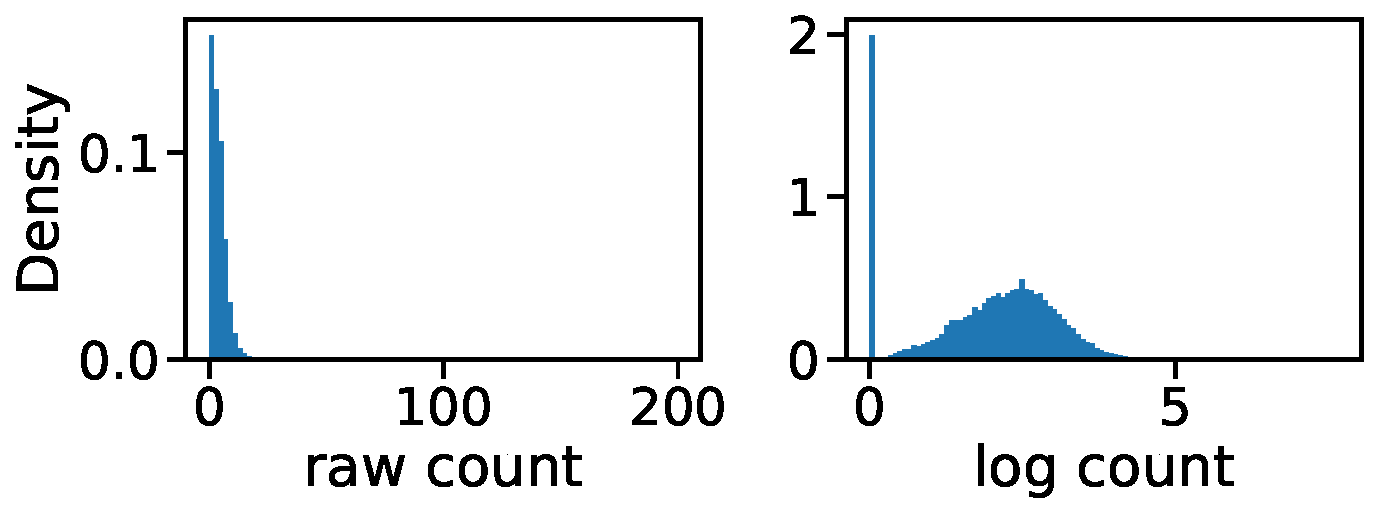
\includegraphics[width=\textwidth]{images/kmers_log_dist.pdf}
\caption{$k$-mer counts are log-normally distributed. A) The frequency of $k$-mer counts over all $k$-mers, over all annotated transcripts in the human genome. B) The distribution in (A), with log-transformed counts.}
\label{fig:logdist}
\end{figure}

\subsection{$k$-mer counting methodologies}

We then asked if we could devise a $k$-mer counting strategy that yielded more consistent estimates of correlations between two sequences, in a way that is sensible and mathematically tractable. The primary difficulty is the addition of a $z$-score calculation step within SEEKR, which transforms the data in a way that suppresses the influence of naturally frequent or depleted $k$-mers within a reference set, \emph{e.g.} the transcriptome. 

Within our \emph{Rsx} analysis in Chapter 2, we originally noticed that the $z$-scores themselves were log-normally distributed, and so we log-transformed the $z$-scores after shifting all values by equation \ref{eq:seekrrsx} (Sprague et al, 2019).

\begin{equation}
M_{ij}^* = \log_2{\left(M_{ij} + |\min{M}|+1\right)}
\label{eq:seekrrsx}
\end{equation}


Where $M$ is the SEEKR $z$-score matrix, $i$ is the row, $j$ is the column ($M_{ij}$ is then the coordinates of a single data point in $M$), and $\min{M}$ is the smallest value in the matrix $M$. This translation of the data allows for the calculation of the log. An issue with this methodology, however, is that there is no clear best choice of value to add to each data point in $M$, due to the log-transform. The goal, therefore, was to add the smallest possible value to each data-entry without destroying the linear relationship between row vectors. Each row within a SEEKR matrix represents the vector of $k$-mer frequencies within a single sequence, and the correlation step in SEEKR calculates the Pearson correlation between all pair-wise combinations of rows within $M$.

Below, we iterate through a series of algorithms for generating the final SEEKR matrix from which correlations will be calculated. 

\subsubsection{Method 1. Kirk et al. 2018}

The first method we outline is the original algorithm published in \emph{Kirk et al.}. Here, we first count the occurrence of each $k$-mer in a sequence. This count is then normalized to a per-kB count by dividing each $k$-mer count by the length of the sequence and multiplying by 1000. This process is then repeated for a reference set of sequences, \emph{e.g.} the transcriptome, and the mean frequency and standard deviation for each $k$-mer over the reference set are calculated. From there, each frequency count in the SEEKR frequency matrix is transformed using Equation \ref{eq:zscore}. 

\begin{table}[h]
\begin{center}
\begin{tabular}{llllll}
&MXA & MXB                   & MXC                  & HXD                   & MXE                                         \\
KR1 & -0.048 & 0.266   & 0.001 & 0.146    & -0.117 \\
KR2 & 0.085   & -0.089  & -0.111  & -0.024 & 0.147  \\
KR3 & -0.041 & -0.119   & -0.009 & -0.021 & 0.267   \\
KR4 & 0.180   & -0.114 & -0.081  & 0.087   & 0.294 
\end{tabular}
\caption{SEEKR Pearson correlations between the tandem repeats of \emph{Xist} and \emph{Rsx}. Correlations were calculated as in \emph{Kirk et al.}, 2018.}
\label{tbl:kmers1}

\end{center}
\end{table}

From here, the pair-wise correlations of each sequence's $k$-mer profile, \emph{i.e.} the row vector of $k$-mer $z$-scores, are calculated. For each of the methods outlined in this chapter, we compare the tandem repeats of \emph{XIST} against the tandem repeats of \emph{Rsx} as in \emph{Sprague et al.}. The correlations for this algorithm are shown in Table \ref{tbl:kmers1}.

\subsubsection{Method 2. Sprague et al. 2019}

\begin{table}[h]
\begin{center}
\begin{tabular}{llllll}
&MXA & MBX                  & MXC                  & HXD                  & MXE                                        \\
KR1 & -0.021 & 0.325   & 0.038 & 0.193   & -0.163 \\
KR2 & 0.084  & -0.122  & -0.122 & -0.013 & 0.145  \\
KR3 & -0.077   & -0.093 & 0.014 & -0.023 & 0.249   \\
KR4 & 0.210   & -0.114 & -0.068 & 0.112   & 0.398
\end{tabular}
\caption{SEEKR Pearson correlations between the tandem repeats of \emph{Xist} and \emph{Rsx}. Correlations were calculated as in \emph{Sprague et al.}, 2019.}
\label{tbl:kmers2}

\end{center}
\end{table}

The second method outlined is the algorithm published in \emph{Sprague et al.}. The $k$-mers are counted exactly as in \emph{Kirk et al.}, however we additionally calculated the $log_2$ of the $z$-scores using Equation \ref{eq:seekrrsx}. Tandem repeat comparisons that were highly correlated as in Method 1 saw large increases in correlation using this method, whereas uncorrelated regions saw little change (Table \ref{tbl:kmers2}). 




\subsubsection{Method 3. Row-wise addition to z-scores}

A concern when translating data, as in Equation \ref{eq:seekrrsx}, is the unequal effect it has when calculating the log of the data. Typically, Pearson correlation is translation invariant, \emph{i.e.} the addition of any constant to all elements of a vector does not affect its correlation with another vector. This is because the calculation of the Peasron correlation involves 0-mean centering each vector, which negates the addition or multiplication of any constant. Another intuition is that moving a scatter plot around on a graph changes the location of the data points, but it doesn't change the relative relationship between data points (slope of best fit). 

\begin{table}[ht]
\begin{center}
\begin{tabular}{llllll}
&MXA & MXB                   & MXC                  & HXD                  & MXE                                  \\
KR1 & -0.017 & 0.327   & 0.042  & 0.197    & -0.163 \\
KR2 & 0.088   & -0.124 & -0.120 & -0.009 & 0.147 \\
KR3 & -0.079  & -0.090 & 0.016 & -0.022 & 0.246 \\
KR4 & 0.214    & -0.110 & -0.066  & 0.115   & 0.404
\end{tabular}
\caption{SEEKR Pearson correlations between the tandem repeats of \emph{Xist} and \emph{Rsx}. Correlations were calculated as in \emph{Sprague et al.}, 2018., except that instead of the minimum of the $z$-score matrix being added, the minimum of each row was added to all values within the row.}
\label{tbl:kmers3}
\end{center}
\end{table}

However, the inclusion of a log-transformation step alters the linear relationship of the data depending on how far the data is from 0. Therefore, it is ideal to add the smallest possible constant to each entry in the matrix. \emph{Sprague et al.} added the minimum of the entire matrix to each $z$-score, however adding the minimum of each row to all values within that row allows for the addition of the smallest possible value such that the log can be taken, without altering the relationship between the $k$-mer counts within a given sequence. The results were similar to those in Method 2, except with further increases in correlation between high correlated domains such as KR4-MXE and KR1-MXB (Table \ref{tbl:kmers3}). 


\subsubsection{Method 4: Column-wise addition to z-scores}

To illustrate the point that the value added to the SEEKR matrix must be constant within a row, here we repeat what was done in Method 3, but instead of adding the minimum of each row to all values within that row, we take the minimum of each column and add that value to each element within the column.

\begin{table}[ht]
\begin{center}
\begin{tabular}{llllll}
&MXA & MXB                  & MXC                   & HXD                 & MXE                                      \\
KR1 & -0.048 & 0.348    & 0.093 & 0.284  & -0.098 \\
KR2 & 0.057  & -0.046 & 0.034 & 0.201 & 0.261  \\
KR3 & -0.061 & -0.015 & 0.144 & 0.173 & 0.347  \\
KR4 & 0.147   & -0.094  & 0.044 & 0.241 & 0.451 
\end{tabular}
\caption{SEEKR Pearson correlations between the tandem repeats of \emph{Xist} and \emph{Rsx}. Correlations were calculated as in \emph{Sprague et al.}, 2018., except that instead of the minimum of the $z$-score matrix being added, the minimum of each column was added to all values within the column.}
\label{tbl:kmers4}
\end{center}
\end{table}
As an example, consider the hypothetical SEEKR $z$-score matrix in Table \ref{tbl:ex1}. After applying the transformation described in this section, all values are greater than 0 which allows for the log-transform of the data (Table \ref{tbl:ex2}. However, the $k$-mer frequencies within each sequence have become jumbled. Consider the relationship between A and T in seq1. Prior to the transformation, T was clearly depleted relative to A in seq1, with $z$-scores of -2 and 0 respectively. 
\begin{table}[h!]
\begin{center}
\begin{tabular}{lllll}
&A & T                   & C                  & G                                                    \\
seq1 & 0 & -2   & 5  & -3 \\
seq2 & 0   & 1 & 3 & -2 
\end{tabular}
\caption{A hypothetical SEEK $z$-score matrix.}
\label{tbl:ex1}
\end{center}
\end{table}
After the transformation, the SEEKR matrix is now indicating that A and T are equally frequent in seq1. Likewise, G was depleted relative to A in both seq1 and seq2, but after the operation is now enriched relative to A.  This operation therefore does not make sense, as we are only trying to move the data to be positive, such that we can calculate the log. While the correlations look promising in Table \ref{tbl:kmers4}, the scatter plots of the $k$-mer counts show that  significant aberration has been introduced to the data relative to Methods 1,2 and 3 (Figure \ref{fig:2plots}). 


\begin{table}[h!]
\begin{center}
\begin{tabular}{lllll}
&A & T                   & C                  & G                                                    \\
seq1 & 1 & 1   & 7  & 1 \\
seq2 & 1   & 4 & 5 & 2  
\end{tabular}
\caption{The same matrix as in Table \ref{tbl:ex1} but transformed by adding the minimum of each column to all values within that column, then adding 1 such that all values are greater than 0.}
\label{tbl:ex2}
\end{center}
\end{table}

\begin{figure}[h]
\centering
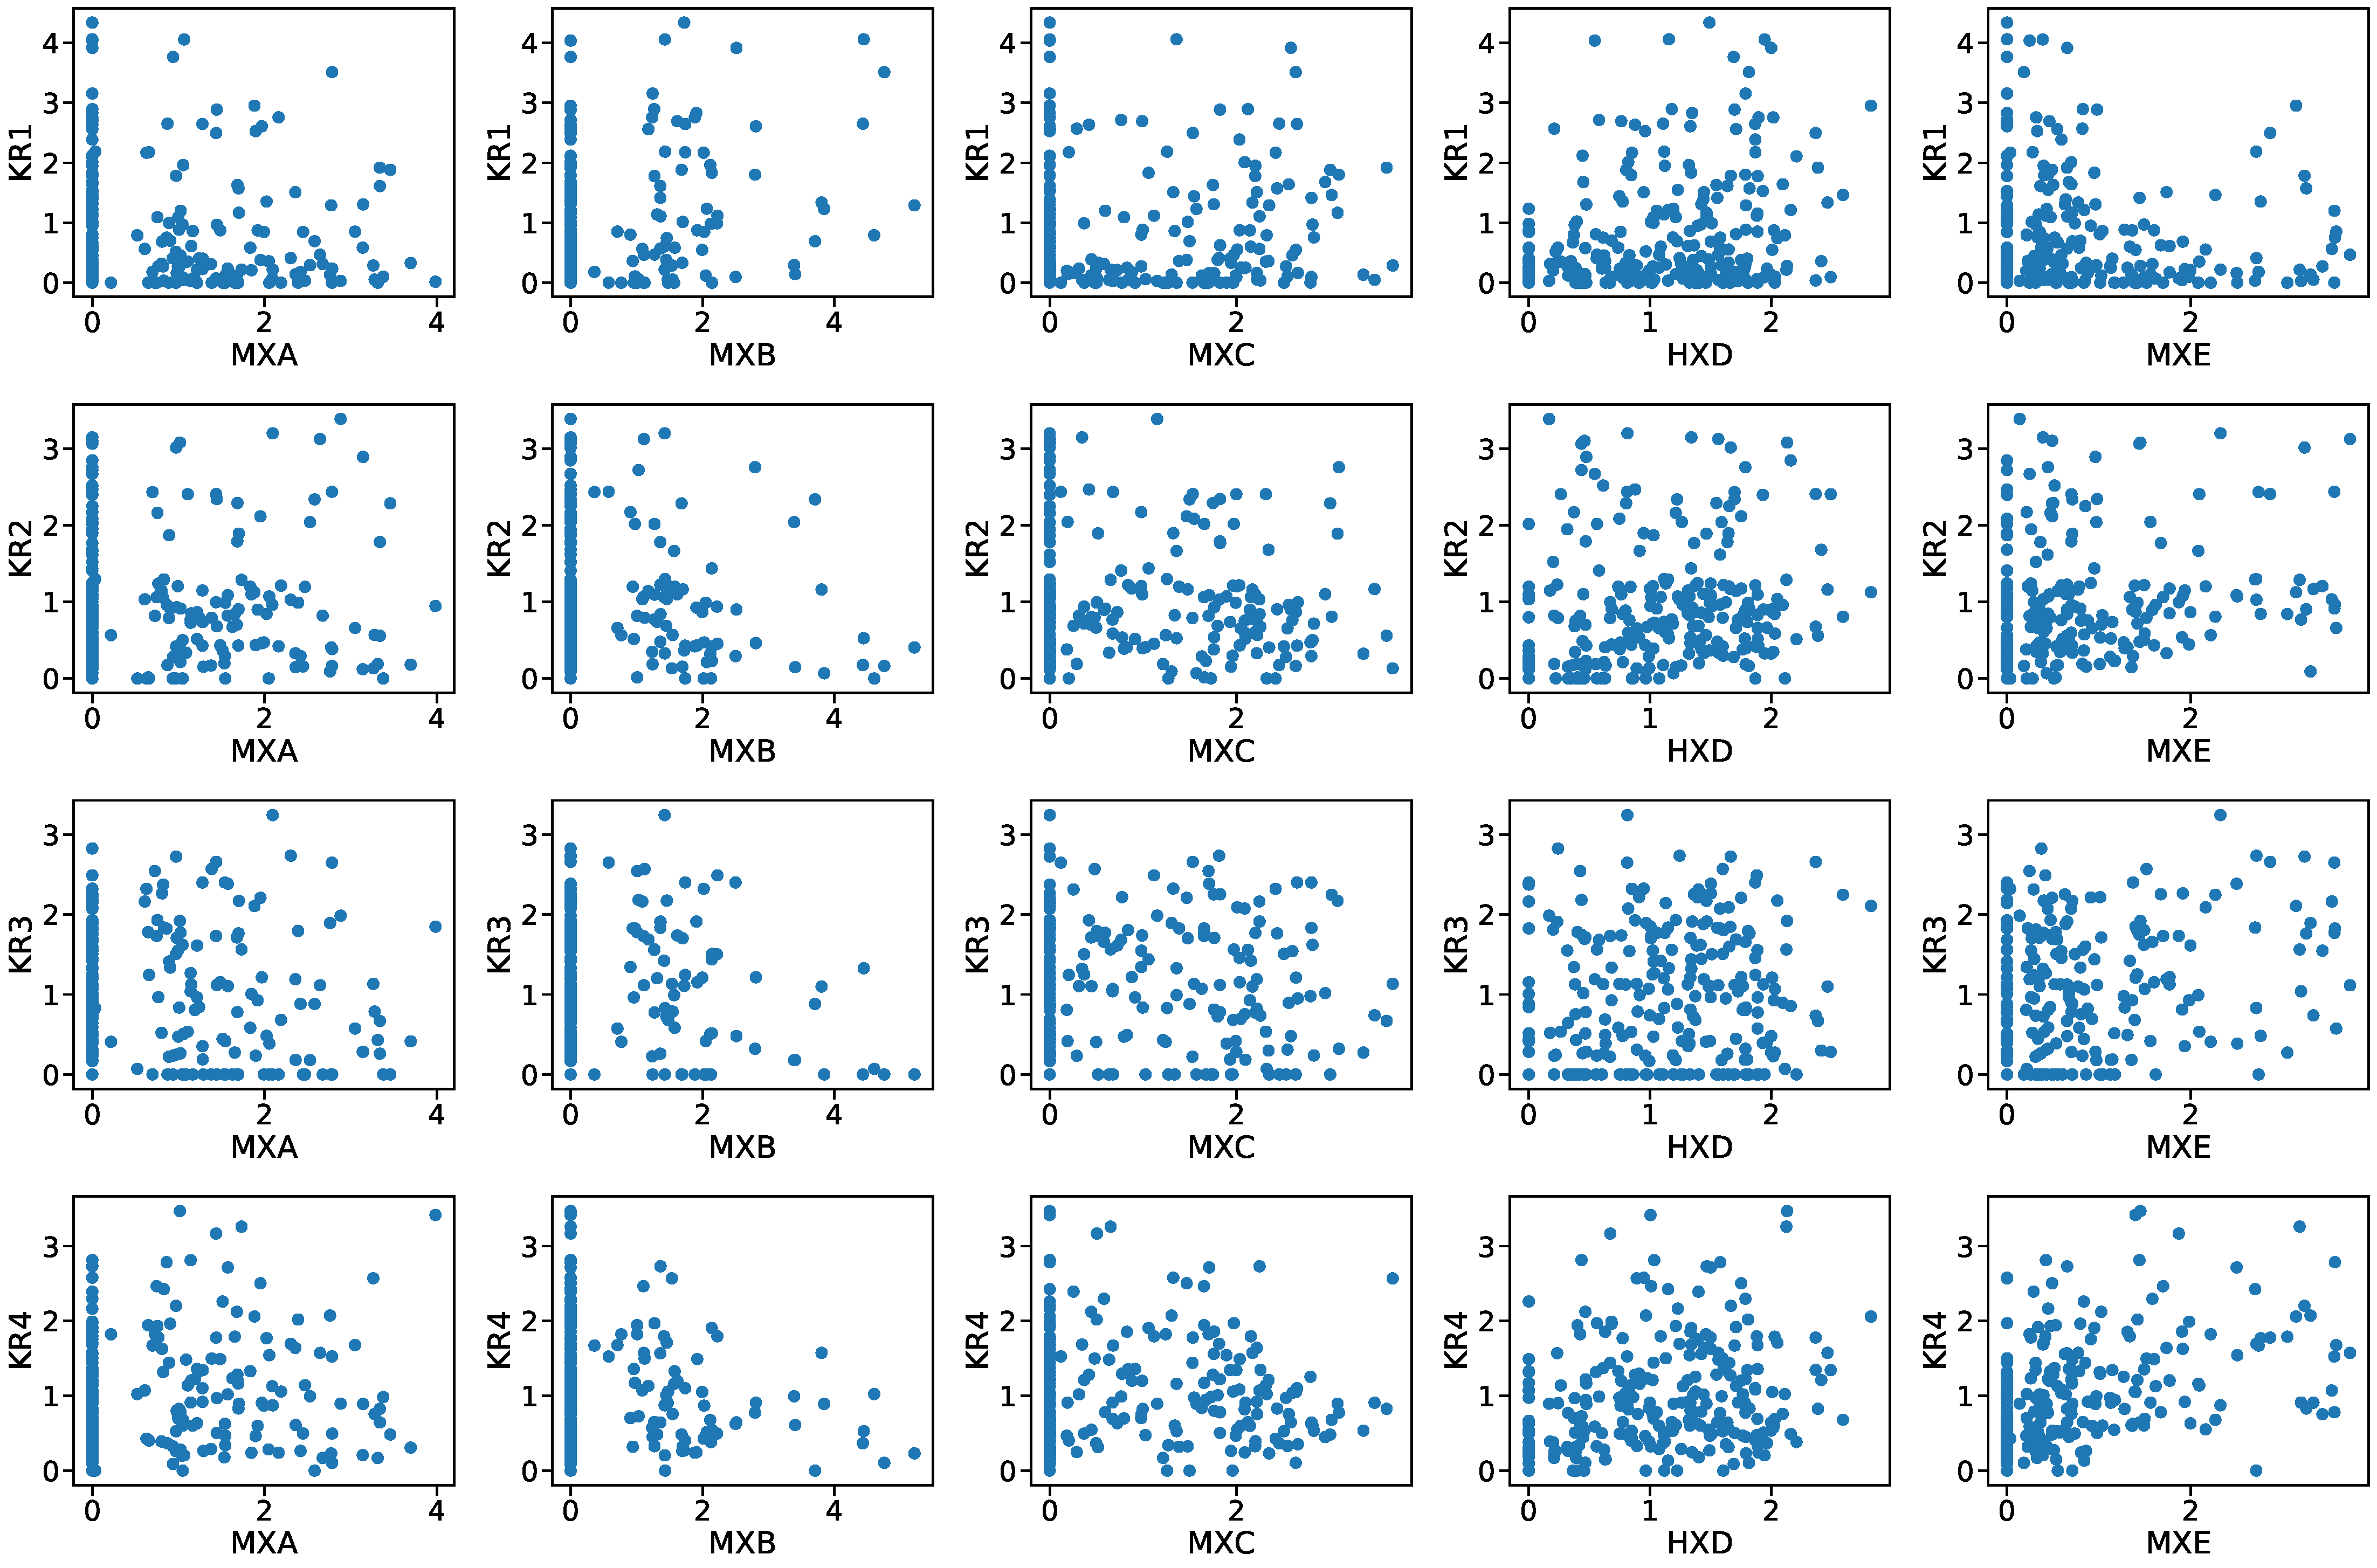
\includegraphics[width=\textwidth]{images/2_figs.pdf}
\caption{Scatter plots of SEEKR $z$-scores for all pair-wise comparisons between MXA,MXB,HXD,MXE and KR1,KR2,KR3, and KR4 using Method 4. Each dot represents a $k$-mer $z$-score for both transcripts being compared (x,y axis).}
\label{fig:2plots}
\end{figure}

\subsubsection{Method 5: Pseudo-count to raw counts}

A more natural transformation of the data is to take the logarithm of the raw count data, which is guaranteed to be $\geq 0$. A potential downside with this approach is that adding 1 to raw counts has a differential effect on sequences of different lengths, \emph{i.e.} adding +1 to the count of all $k$-mers in a sequence that is 200bp long has a larger effect on the frequencies than a 10,000bp sequence. Therefore, we tried two different approaches. In Method 5, we added +1 to the raw counts of the data, length normalized the counts, and then took the log-transform, followed by $z$-score calculation as in \emph{Kirk et al.} (Table \ref{tbl:kmers5}).

\begin{table}[ht]
\begin{center}
\begin{tabular}{llllll}
&MXA & MXB                  & MXC                  & HXD                  & MXE                                         \\
KR1 & -0.068 & 0.232    & 0.024  & 0.181   & -0.179 \\
KR2 & -0.074 & -0.295 & -0.087 & 0.071  & 0.126  \\
KR3 & -0.170 & -0.170 & 0.063   & 0.001 & 0.205  \\
KR4 & 0.119  & -0.175  & -0.014 & 0.148   & 0.387
\end{tabular}
\caption{SEEKR Pearson correlations between the tandem repeats of \emph{Xist} and \emph{Rsx}. Correlations were calculated adding a pseudo-count to the raw count data (Method 5).}
\label{tbl:kmers5}
\end{center}
\end{table}

\subsubsection{Method 6: Length normalized pseudo-count}
The second method was to add 1 after length normalizing the $k$-mer counts per kB, effectively making the pseudo-count equivalent between transcripts of different lengths, and then going through SEEKR as before. The results are shown in Table \ref{tbl:kmers6}. This latter method of adding a pseudo-count posterior to length normalization is the method we chose to continue using with SEEKR going forward, as the mathematics are straigt forward and are best suited to the data at hand, as well as yielding strong results between regions known to share similar function and $k$-mer frequencies (Figure \ref{fig:9plots}). 

\begin{table}[ht]
\begin{center}
\begin{tabular}{llllll}
&MXA & MXB                   & MXC                  & HXD                  & MXE                                        \\
KR1 & -0.013 & 0.335  & 0.059  & 0.200  & -0.163 \\
KR2 & 0.039   & -0.152 & -0.080  & -0.007 & 0.135  \\
KR3 & -0.102   & -0.067 & 0.076  & -0.025 & 0.220   \\
KR4 & 0.249   & -0.078 & 0.015 & 0.150  & 0.431 
\end{tabular}
\caption{SEEKR Pearson correlations between the tandem repeats of \emph{Xist} and \emph{Rsx}. Correlations were calculated using a length normalized pseudo-count (Method 6).}
\label{tbl:kmers6}
\end{center}
\end{table}

\begin{figure}[h]
\centering
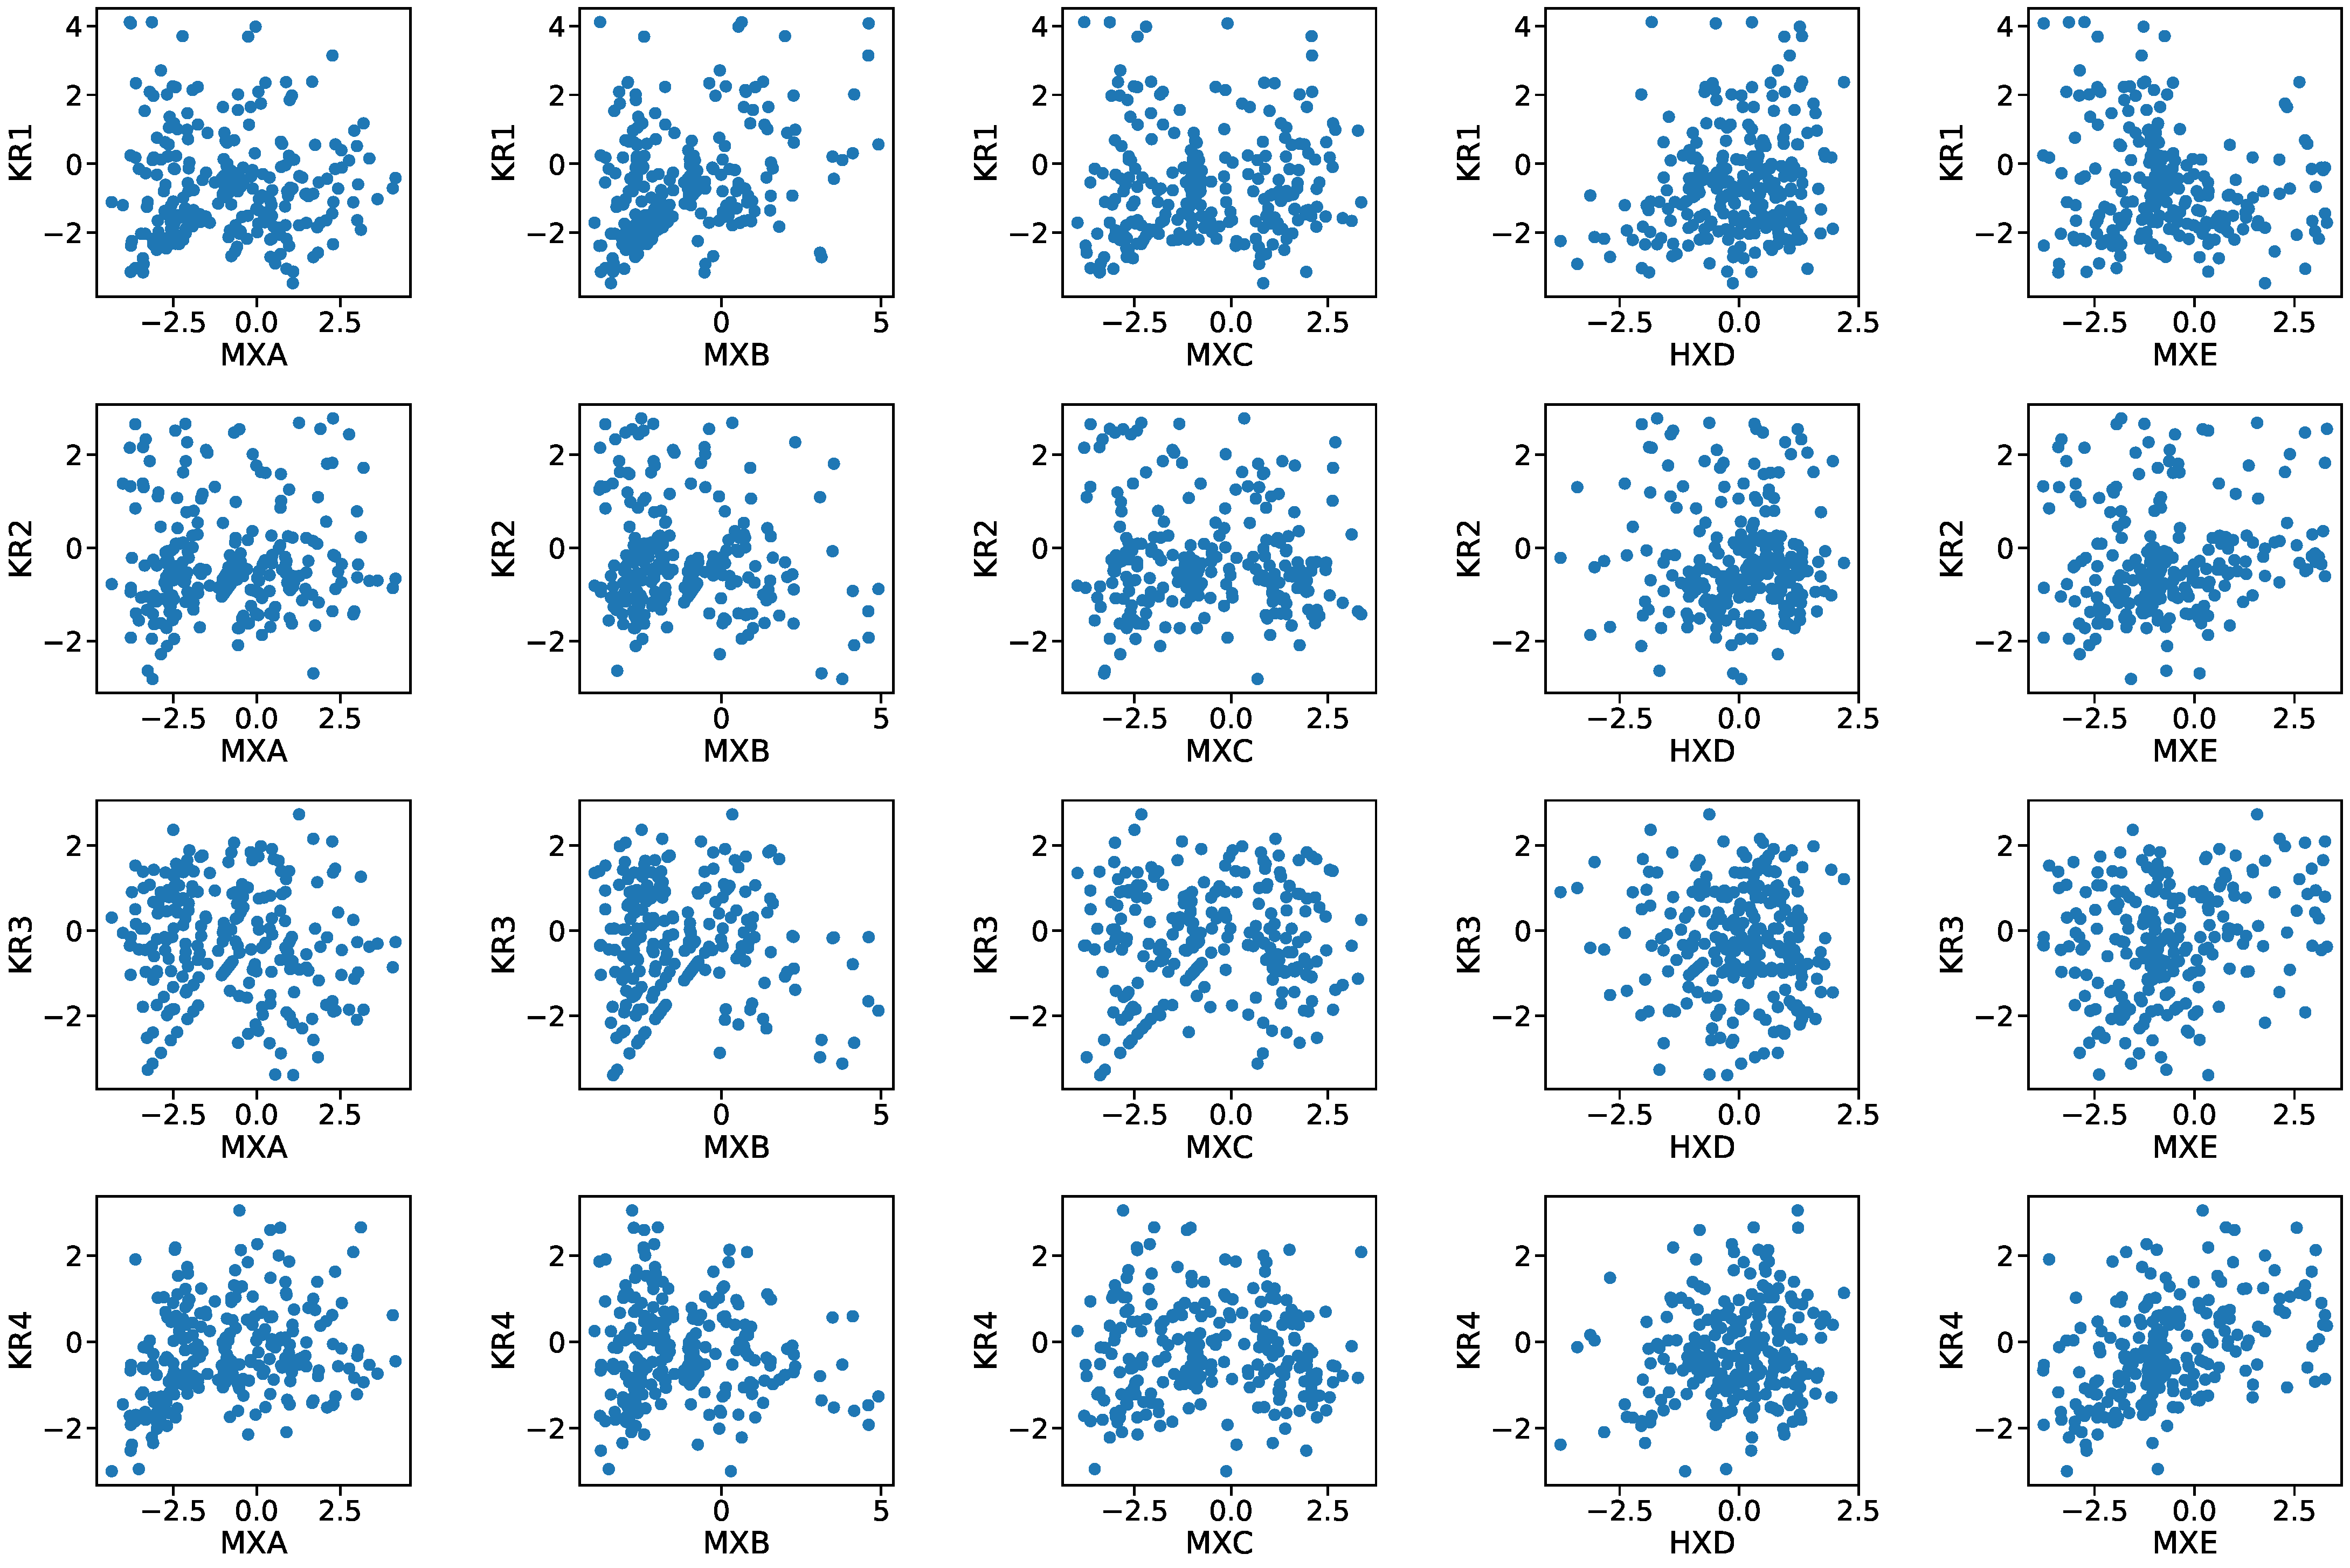
\includegraphics[width=\textwidth]{images/9_figs.pdf}
\caption{Scatter plots of SEEKR $z$-scores for all pair-wise comparisons between MXA,MXB,HXD,MXE and KR1,KR2,KR3, and KR4 using Method 6. Each dot represents a $k$-mer $z$-score for both transcripts being compared (x,y axis).}
\label{fig:9plots}
\end{figure}

\clearpage

\section{Methods}

\subsection{$k$-mer count distributions}

For a given sequence, \emph{e.g.}``seq1", we counted how many times we observed each $k$-mer. This yields a vector representing $\{c_{AAA},c_{AAT},\dots\,c_{GGG}\}$, where $c_{kmer}$ is the number of observed counts for that $k$-mer. We then calculated the frequency distribution of counts in a sequence, over all $k$-mers. \emph{E.g.}, if the $k$-mers AAA and GGG had counts $c_{AAA} = 5$ and $c_{GGG} = 5$, and no other $k$-mers had a count of 5 in ``seq1", then we would record a frequency of 2 for the number of times we observed a count of 5 in ``seq1". These observed frequencies were calculated for each transcript and then summed, \emph{e.g.} if we observed a count of 5 twice in ``seq1" and 10 times in ``seq2", then the marginal frequency of a count of 5 over those two sequences is 15.

$$
P(\texttt{frequency}) = \sum_{\texttt{k-mers}}{\sum_{\texttt{sequences}}{P(\texttt{frequency,sequences,k-mers)}}}
$$

\subsection{SEEKR Data Sources}
For each of the analyses above, we used the following transcript annotations. For \emph{XIST}, we used Mouse A-repeat (MXA), mouse B-repeat (MXB), human D-repeat (HXD), and mouse E-repeat (MXE) as annotated in \cite{Brockdorff10TheNucleus.}. For the \emph{Rsx} repeats, we used the koala \emph{Rsx} 1,2,3, and 4 repeats as defined in \cite{Sprague2019NonlinearDomains}. For the reference set of sequences within SEEKR, used the GENCODE (M14) annotated set of spliced lncRNA transcripts in the mouse transcriptome. 


\begin{singlespace}
\printbibliography
\end{singlespace}
\chapter{Conclusion}
The non-coding portion of our genome represents a significant portion of the mammalian transcriptome \cite{Rinn2012GenomeRNAs}. Small non-coding RNAs are relatively well understood \cite{Rinn2012GenomeRNAs}, however they make up only a fraction of annotated non-coding RNA transcripts. Despite representing a large fraction of known transcripts in the mammalian genome, we have solid understanding of only a handful of lncRNAs. \emph{XIST} was discovered in 1992 \cite{Brown10TheNucleus.}, and yet we are still learning how exactly Xist functions within the cell \cite{Schertzer2019LncRNA-InducedDNA,DaRocha2017NovelConformation}. 

A significant frustration is the unclear sequence to function relationship in lncRNAs. This relationship has long been understood in protein coding genes \cite{Whisstock2003PredictionStructure} and has been facilited by numerous bioinformatics tools that can rapidly predict relationships between protein coding genes \cite{Altschul1990BasicTool,Smith1981IdentificationSubsequences,Wheeler2013Nhmmer:HMMs,Yi2013Co-phylog:Organisms,Qi2004WholeApproach}. 

\begin{singlespace}
\printbibliography[heading=bibintoc,title={References}]
\end{singlespace}


\end{document}
